% Anonymous ICLR 2027 manuscript. Build with ./build.sh. Numerical tables are generated.
\documentclass{article}
\usepackage{iclr2027_conference,times}

\usepackage[utf8]{inputenc}
\usepackage[T1]{fontenc}
\usepackage{amsmath,amssymb,amsfonts}
\usepackage{graphicx}
\usepackage{booktabs}
\usepackage{multirow}
\usepackage{array}
\usepackage{xcolor}
\usepackage{tikz}
\usetikzlibrary{positioning,arrows.meta,calc,fit,backgrounds,shapes.geometric}
\usepackage{caption}
\captionsetup{font=small,labelfont=bf}
\usepackage{hyperref}
\hypersetup{hidelinks}
\usepackage{url}
\usepackage{microtype}
\usepackage{placeins}
\usepackage{float}
\usepackage{enumitem}
\setlist{nosep,leftmargin=*}

\graphicspath{{figures/}}
%
% macros.tex -- notation for the NM-ROM methods section.
% Symbol conventions (kept deliberately disjoint from the old submission, which
% overloaded K for both the discrete operator and a latent-adjacent quantity):
%   N  intervals per axis        n  interior unknowns
%   R  spatial bank width        k  latent dimension
%   M  number of retained weak tests    m  number of empirical-quadrature nodes

\newcommand{\Real}{\mathbb{R}}
\newcommand{\Nat}{\mathbb{N}}

% --- discrete objects -------------------------------------------------------
\newcommand{\Aop}{A}                    % fixed linear discrete operator
\newcommand{\bank}{G}                   % frozen spatial bank, n x R
\newcommand{\head}{h_\theta}            % nonlinear coefficient map, R^k -> R^R
\newcommand{\tests}{P}                  % weak test matrix, M x n
\newcommand{\rowscale}{\Lambda}         % diagonal row scaling
\newcommand{\lift}{u_{g}}               % boundary lift
\newcommand{\bcmask}{\mu}               % boundary mask / vanishing factor
\newcommand{\latent}{z}
\newcommand{\umanifold}{u}

% --- operators and norms ----------------------------------------------------
\newcommand{\jac}[1]{J_{#1}}
\newcommand{\dhead}{D\head}
\newcommand{\norm}[1]{\lVert #1 \rVert}
\newcommand{\normF}[1]{\lVert #1 \rVert_{F}}
\newcommand{\inner}[2]{\langle #1, #2 \rangle}
\newcommand{\T}{^{\top}}
\newcommand{\Tr}{\operatorname{tr}}
\newcommand{\diag}{\operatorname{diag}}
\newcommand{\rank}{\operatorname{rank}}
\newcommand{\argmin}{\operatorname*{arg\,min}}

% --- residuals --------------------------------------------------------------
\newcommand{\rfull}{r}                  % full discrete residual
\newcommand{\rweak}{r_{w}}              % weak (projected, row-scaled) residual
\newcommand{\station}[2]{\eta(#1,#2)}   % normalized-gradient stationarity measure

% --- placeholders for generated numbers -------------------------------------
% Every numeric value in this manuscript must come from a generator script that
% reads the run JSONs. \todo marks a slot that the generator has not yet filled.
\newcommand{\todo}[1]{{\color{red}\textbf{[\,#1\,]}}}
\newcommand{\gen}[1]{\todo{pending: #1}}

% Subscripted variants (the base macros already carry a subscript, so
% \head_a / \rweak_n would be a double subscript).
\newcommand{\headc}[1]{h_{\theta,#1}}   % one component of the head output
\newcommand{\rweakn}[1]{r_{w,#1}}       % the weak residual of time step #1

%
% GENERATED by paper/gen_tables.py -- do not edit.
% Every prose number in the manuscript is one of these macros.
\newcommand{\nAblBurgersBestFound}{2.5447}
\newcommand{\nAblBurgersFloor}{0.3918}
\newcommand{\nAblBurgersFree}{0.6027}
\newcommand{\nAblBurgersFreeMs}{2417.6}
\newcommand{\nAblBurgersLinear}{56.9296}
\newcommand{\nAblBurgersNeural}{2.5629}
\newcommand{\nAblBurgersNeuralMs}{47.6}
\newcommand{\nAblBurgersPodOneTwentyEight}{10.1198}
\newcommand{\nAblBurgersPodOneTwentyEightMs}{328.3}
\newcommand{\nAblBurgersPodSixteen}{61.6503}
\newcommand{\nAblBurgersQuad}{31.8276}
\newcommand{\nAblBurgersReductionOverFloor}{6.5}
\newcommand{\nAblBurgersSolverGapPp}{0.018}
\newcommand{\nAblPoissonBestFound}{6.0926}
\newcommand{\nAblPoissonDst}{0.0007}
\newcommand{\nAblPoissonDstMs}{4.341}
\newcommand{\nAblPoissonFloor}{2.3148}
\newcommand{\nAblPoissonFree}{2.3274}
\newcommand{\nAblPoissonLinear}{17.2966}
\newcommand{\nAblPoissonNeural}{6.0927}
\newcommand{\nAblPoissonNeuralMs}{5.843}
\newcommand{\nAblPoissonPodOneTwentyEight}{4.3452}
\newcommand{\nAblPoissonPodOneTwentyEightMs}{5.930}
\newcommand{\nAblPoissonPodSixteen}{20.0548}
\newcommand{\nAblPoissonQthirtytwo}{4.6670}
\newcommand{\nAblPoissonQthirtytwoMs}{7.317}
\newcommand{\nAblPoissonQuad}{16.6303}
\newcommand{\nBlockBlockBudgetExits}{0}
\newcommand{\nBlockBlockErr}{2.1489}
\newcommand{\nBlockBlockMs}{619.2}
\newcommand{\nBlockJointBudgetExits}{6}
\newcommand{\nBlockJointErr}{2.1489}
\newcommand{\nBlockJointMs}{1119.7}
\newcommand{\nCgLshapeCgTol}{$10^{-10}$}
\newcommand{\nCgLshapeMeshes}{$64^2$, $128^2$, $256^2$, $512^2$}
\newcommand{\nCgLshapePcgRatioMax}{990.8}
\newcommand{\nCgLshapePcgRatioMin}{3.6}
\newcommand{\nCgLshapeSpeedupMax}{14.9}
\newcommand{\nCgLshapeSpeedupMin}{2.9}
\newcommand{\nCgPoissonCgMsTwoFiftySix}{38.0}
\newcommand{\nCgPoissonDstFasterMax}{4.0}
\newcommand{\nCgPoissonDstFasterMin}{1.3}
\newcommand{\nCgPoissonSpeedupMax}{23.4}
\newcommand{\nCgPoissonSpeedupMin}{3.7}
\newcommand{\nColdCapEightNearest}{6.09}
\newcommand{\nColdCapEightZero}{30.03}
\newcommand{\nColdCapTwelveNearest}{6.09}
\newcommand{\nColdCapTwelveZero}{6.09}
\newcommand{\nColdCapTwoNearest}{6.80}
\newcommand{\nColdCapTwoZero}{91.88}
\newcommand{\nColdConvNearest}{6.09}
\newcommand{\nColdConvZero}{6.09}
\newcommand{\nColdMesh}{1024}
\newcommand{\nColdStarts}{nearest, zero}
\newcommand{\nEqtopBar}{0.116}
\newcommand{\nEqtopBarOrigin}{the held-out $\rho$ of the incumbent $q{=}0$ rule at the state carrying the first-interval penalty, measured in the q-diag cell and adopted as the primary bar in the q-ridge design before any certification job ran; the tight bar was declared before b-eqtop ran}
\newcommand{\nEqtopConfirmedCount}{3}
\newcommand{\nEqtopConfirmedRungs}{0, 16, 32}
\newcommand{\nEqtopCostRatioMax}{0.21}
\newcommand{\nEqtopCostRatioMin}{0.18}
\newcommand{\nEqtopLadderConverged}{yes}
\newcommand{\nEqtopLadderCostSpan}{12.23}
\newcommand{\nEqtopLadderErrSpan}{3.51}
\newcommand{\nEqtopLadderFirstErr}{1.8891}
\newcommand{\nEqtopLadderFirstMs}{59.1}
\newcommand{\nEqtopLadderLastErr}{0.5389}
\newcommand{\nEqtopLadderLastMs}{722.2}
\newcommand{\nEqtopLadderMonotone}{yes}
\newcommand{\nEqtopMarginalCount}{3}
\newcommand{\nEqtopMarginalRungs}{64 (2/6), 128 (4/5), 256 (1/5)}
\newcommand{\nEqtopParentOneTwentyEightRho}{0.1908}
\newcommand{\nEqtopParentTwoFiftySixRho}{0.1678}
\newcommand{\nEqtopPendingJob}{none}
\newcommand{\nEqtopPrimaryOneTwentyEight}{yes}
\newcommand{\nEqtopPrimaryOneTwentyEightM}{2048}
\newcommand{\nEqtopPrimaryOneTwentyEightRho}{0.0669}
\newcommand{\nEqtopPrimaryOneTwentyEightStates}{64}
\newcommand{\nEqtopPrimaryTwoFiftySix}{yes}
\newcommand{\nEqtopPrimaryTwoFiftySixM}{2048}
\newcommand{\nEqtopPrimaryTwoFiftySixRho}{0.1074}
\newcommand{\nEqtopPrimaryTwoFiftySixStates}{64}
\newcommand{\nEqtopQsixtyFourArchivedRho}{0.0531}
\newcommand{\nEqtopQsixtyFourRedrawRho}{0.1220}
\newcommand{\nEqtopSpreadMax}{9.6}
\newcommand{\nEqtopSpreadMin}{1.4}
\newcommand{\nEqtopStaticWorstFit}{1.5e-04}
\newcommand{\nEqtopStaticWorstOverBar}{4.0}
\newcommand{\nEqtopStaticWorstQ}{256}
\newcommand{\nEqtopStaticWorstRho}{0.462}
\newcommand{\nEqtopStatus}{final}
\newcommand{\nEqtopStatusQOneTwentyEight}{marginal (4 of 5 draws pass)}
\newcommand{\nEqtopStatusQSixteen}{confirmed (3 of 3 re-draws)}
\newcommand{\nEqtopStatusQSixtyFour}{marginal (2 of 6 draws pass)}
\newcommand{\nEqtopStatusQThirtyTwo}{confirmed (2 of 2 re-draws)}
\newcommand{\nEqtopStatusQTwoFiftySix}{marginal (1 of 5 draws pass)}
\newcommand{\nEqtopStatusQZero}{confirmed (3 of 3 re-draws)}
\newcommand{\nEqtopTightBar}{0.06}
\newcommand{\nEqtopTopDenseErr}{0.5194}
\newcommand{\nEqtopTopDenseMs}{3915.1}
\newcommand{\nEqtopTopDraws}{1 of 5}
\newcommand{\nEqtopTopEqErr}{0.5389}
\newcommand{\nEqtopTopEqMs}{722.2}
\newcommand{\nEqtopTopM}{2048}
\newcommand{\nEqtopTopOldRuleErr}{1.0361}
\newcommand{\nEqtopTopOldRuleRho}{0.1678}
\newcommand{\nEqtopTopRedrawMin}{0.182}
\newcommand{\nEqtopTopRedrawRange}{0.130--0.242}
\newcommand{\nEqtopTopRho}{0.1074}
\newcommand{\nHeatBankErrTenTwentyFour}{1.68}
\newcommand{\nHeatBankErrTwoFiftySix}{1.68}
\newcommand{\nHeatBankMsTenTwentyFour}{0.56}
\newcommand{\nHeatBankMsTwoFiftySix}{0.14}
\newcommand{\nHeatBankOverHeadCostTenTwentyFour}{22}
\newcommand{\nHeatBankOverHeadCostTwoFiftySix}{86}
\newcommand{\nHeatFomMsTenTwentyFour}{1.03}
\newcommand{\nHeatFomMsTwoFiftySix}{0.21}
\newcommand{\nHeatHeadErrTenTwentyFour}{4.56}
\newcommand{\nHeatHeadErrTwoFiftySix}{4.56}
\newcommand{\nHeatHeadMsTenTwentyFour}{12.3}
\newcommand{\nHeatHeadMsTwoFiftySix}{11.9}
\newcommand{\nLinearBankOverPodMax}{4.0}
\newcommand{\nLinearBankOverPodMin}{3.4}
\newcommand{\nLshapeBestFloor}{0.6650}
\newcommand{\nLshapeBestFloorCommon}{1.6155}
\newcommand{\nLshapeCheapestFomErrFiveTwelve}{0.385}
\newcommand{\nLshapeCheapestFomErrOneTwentyEight}{0.000}
\newcommand{\nLshapeCheapestFomErrSixtyFour}{0.000}
\newcommand{\nLshapeCheapestFomErrTwoFiftySix}{0.000}
\newcommand{\nLshapeCheapestFomFiveTwelve}{CG $10^{-2}$}
\newcommand{\nLshapeCheapestFomMoreAccurateFiveTwelve}{5.5}
\newcommand{\nLshapeCheapestFomMoreAccurateOneTwentyEight}{exact}
\newcommand{\nLshapeCheapestFomMoreAccurateSixtyFour}{exact}
\newcommand{\nLshapeCheapestFomMoreAccurateTwoFiftySix}{exact}
\newcommand{\nLshapeCheapestFomMsFiveTwelve}{29.13}
\newcommand{\nLshapeCheapestFomMsOneTwentyEight}{2.48}
\newcommand{\nLshapeCheapestFomMsSixtyFour}{1.28}
\newcommand{\nLshapeCheapestFomMsTwoFiftySix}{8.39}
\newcommand{\nLshapeCheapestFomOneTwentyEight}{sparse direct (SuperLU)}
\newcommand{\nLshapeCheapestFomSixtyFour}{sparse direct (SuperLU)}
\newcommand{\nLshapeCheapestFomTwoFiftySix}{sparse direct (SuperLU)}
\newcommand{\nLshapeDevelopmentWorst}{6.8}
\newcommand{\nLshapeEnrichFloor}{0.6650}
\newcommand{\nLshapeEnrichGain}{1.067}
\newcommand{\nLshapeFiveTwelveBestPod}{POD $k'{=}128$}
\newcommand{\nLshapeFiveTwelveBestPodErr}{2.451}
\newcommand{\nLshapeFiveTwelveBestPodMs}{4.031}
\newcommand{\nLshapeFiveTwelveBestReduced}{head $q{=}64$ (head\_sdf\_R512\_K16)}
\newcommand{\nLshapeFiveTwelveBestReducedErr}{2.123}
\newcommand{\nLshapeFiveTwelveCgErr}{0.385}
\newcommand{\nLshapeFiveTwelveCgMs}{29.13}
\newcommand{\nLshapeFreeErr}{0.7791}
\newcommand{\nLshapeFreeFaster}{1.54}
\newcommand{\nLshapeFreeMoreAccurate}{1.19}
\newcommand{\nLshapeFreeMs}{2.583}
\newcommand{\nLshapeFreeOverFloor}{1.003}
\newcommand{\nLshapeHeadIndepBitwise}{no}
\newcommand{\nLshapeHeadIndepRel}{4.06e-14}
\newcommand{\nLshapeHeadOverPodCostFiveTwelve}{19}
\newcommand{\nLshapeHeadOverPodCostOneTwentyEight}{2}
\newcommand{\nLshapeHeadOverPodCostSixtyFour}{5}
\newcommand{\nLshapeHeadOverPodCostTwoFiftySix}{6}
\newcommand{\nLshapeHeadRatioMax}{5.77}
\newcommand{\nLshapeHeadRatioMin}{2.24}
\newcommand{\nLshapeJobCount}{5}
\newcommand{\nLshapeKsixteenBest}{3.8607}
\newcommand{\nLshapeKthirtytwoBest}{3.1802}
\newcommand{\nLshapeNeuralCheaper}{2.77}
\newcommand{\nLshapeNeuralCheaperFiveTwelve}{7.60}
\newcommand{\nLshapeNeuralCheaperOneTwentyEight}{0.88}
\newcommand{\nLshapeNeuralCheaperSixtyFour}{0.45}
\newcommand{\nLshapeNeuralCheaperTwoFiftySix}{2.77}
\newcommand{\nLshapeNeuralCheaperVsCheapestFiveTwelve}{6.07}
\newcommand{\nLshapeNeuralCheaperVsCheapestOneTwentyEight}{0.88}
\newcommand{\nLshapeNeuralCheaperVsCheapestSixtyFour}{0.45}
\newcommand{\nLshapeNeuralCheaperVsCheapestTwoFiftySix}{2.77}
\newcommand{\nLshapeNeuralErr}{2.131}
\newcommand{\nLshapeNeuralErrFiveTwelve}{2.123}
\newcommand{\nLshapeNeuralErrOneTwentyEight}{2.164}
\newcommand{\nLshapeNeuralErrSixtyFour}{2.300}
\newcommand{\nLshapeNeuralErrTwoFiftySix}{2.131}
\newcommand{\nLshapeNeuralMs}{3.028}
\newcommand{\nLshapeNeuralMsFiveTwelve}{4.801}
\newcommand{\nLshapeNeuralMsOneTwentyEight}{2.806}
\newcommand{\nLshapeNeuralMsSixtyFour}{2.846}
\newcommand{\nLshapeNeuralMsTrend}{2.85 $\to$ 2.81 $\to$ 3.03 $\to$ 4.80}
\newcommand{\nLshapeNeuralMsTwoFiftySix}{3.028}
\newcommand{\nLshapeNeuralNonDomFiveTwelve}{yes}
\newcommand{\nLshapeNeuralNonDomOneTwentyEight}{no}
\newcommand{\nLshapeNeuralNonDomSixtyFour}{no}
\newcommand{\nLshapeNeuralNonDomTwoFiftySix}{yes}
\newcommand{\nLshapeNonDomCount}{7}
\newcommand{\nLshapeNonDomCountFiveTwelve}{8}
\newcommand{\nLshapeNonDomCountOneTwentyEight}{4}
\newcommand{\nLshapeNonDomCountSixtyFour}{1}
\newcommand{\nLshapeNonDomCountTwoFiftySix}{7}
\newcommand{\nLshapeNonDomReduced}{6}
\newcommand{\nLshapeNonDomReducedFiveTwelve}{6}
\newcommand{\nLshapeNonDomReducedOneTwentyEight}{3}
\newcommand{\nLshapeNonDomReducedSixtyFour}{0}
\newcommand{\nLshapeNonDomReducedTwoFiftySix}{6}
\newcommand{\nLshapeOneTwentyEightBestReduced}{POD $k'{=}64$}
\newcommand{\nLshapeOneTwentyEightBestReducedCheaper}{1.08}
\newcommand{\nLshapeOneTwentyEightBestReducedErr}{7.701}
\newcommand{\nLshapeOneTwentyEightCheapRange}{1.08--1.19}
\newcommand{\nLshapeOneTwentyEightReducedErrRange}{7.7--34.6}
\newcommand{\nLshapePodCheaperFiveTwelve}{9.06}
\newcommand{\nLshapePodCheaperOneTwentyEight}{0.90}
\newcommand{\nLshapePodCheaperSixtyFour}{0.47}
\newcommand{\nLshapePodCheaperTwoFiftySix}{2.94}
\newcommand{\nLshapePodCheaperVsCheapestFiveTwelve}{7.23}
\newcommand{\nLshapePodCheaperVsCheapestOneTwentyEight}{0.90}
\newcommand{\nLshapePodCheaperVsCheapestSixtyFour}{0.47}
\newcommand{\nLshapePodCheaperVsCheapestTwoFiftySix}{2.94}
\newcommand{\nLshapePodErrFiveTwelve}{2.451}
\newcommand{\nLshapePodErrOneTwentyEight}{2.483}
\newcommand{\nLshapePodErrSixtyFour}{2.591}
\newcommand{\nLshapePodErrTwoFiftySix}{2.457}
\newcommand{\nLshapePodMsFiveTwelve}{4.031}
\newcommand{\nLshapePodMsOneTwentyEight}{2.764}
\newcommand{\nLshapePodMsSixtyFour}{2.711}
\newcommand{\nLshapePodMsTwoFiftySix}{2.850}
\newcommand{\nLshapePodOverHeadErrFiveTwelve}{15}
\newcommand{\nLshapePodOverHeadErrOneTwentyEight}{15}
\newcommand{\nLshapePodOverHeadErrSixtyFour}{13}
\newcommand{\nLshapePodOverHeadErrTwoFiftySix}{15}
\newcommand{\nLshapePodTwoFiftySixErr}{0.9303}
\newcommand{\nLshapePodTwoFiftySixMs}{3.987}
\newcommand{\nLshapeSdfFloor}{0.7698}
\newcommand{\nLshapeSelectedFloorCommon}{1.6155}
\newcommand{\nLshapeSmoothFloor}{0.7093}
\newcommand{\nLshapeSolve}{in Table~\ref{tab:lshape-solve} ($64^2$--$512^2$, one job per mesh)}
\newcommand{\nLshapeSpluMsFiveTwelve}{36.50}
\newcommand{\nLshapeSpluMsOneTwentyEight}{2.48}
\newcommand{\nLshapeSpluMsSixtyFour}{1.28}
\newcommand{\nLshapeSpluMsTwoFiftySix}{8.39}
\newcommand{\nLshapeValidationGap}{2.5}
\newcommand{\nLshapeValidationWorst}{16.7}
\newcommand{\nLvAllConverged}{yes}
\newcommand{\nLvAnyNeuralNonDom}{no}
\newcommand{\nLvAnyReducedNonDom}{no}
\newcommand{\nLvBankFloorCollapse}{19.00$\times$}
\newcommand{\nLvBankFloorInc}{0.3918}
\newcommand{\nLvBankFloorLow}{7.4455}
\newcommand{\nLvBestFoundInc}{2.5447}
\newcommand{\nLvBestFoundLow}{11.3934}
\newcommand{\nLvBestFoundRatio}{4.48$\times$}
\newcommand{\nLvBudgetExitsTotal}{0}
\newcommand{\nLvCheapestDominatingFom}{\texttt{nt1e-2\_dt01}}
\newcommand{\nLvCheapestDominatingFomErr}{3.90}
\newcommand{\nLvCheapestDominatingFomMs}{14.0}
\newcommand{\nLvControlMonotone}{no}
\newcommand{\nLvDiscMax}{20.9}
\newcommand{\nLvDiscMin}{19.3}
\newcommand{\nLvDiscTight}{20.8}
\newcommand{\nLvFfourDiscRatio}{5.17}
\newcommand{\nLvFreeBank}{7.7940}
\newcommand{\nLvFreeBankMs}{3174.6}
\newcommand{\nLvFtwoFires}{no}
\newcommand{\nLvLadderConverged}{yes}
\newcommand{\nLvLadderCostSpan}{3.25$\times$}
\newcommand{\nLvLadderErrSpan}{1.36$\times$}
\newcommand{\nLvLadderKnobBar}{no}
\newcommand{\nLvLadderMonotone}{yes}
\newcommand{\nLvLadderQtop}{6.6718}
\newcommand{\nLvLadderQtopMs}{1810.3}
\newcommand{\nLvLadderQzero}{9.0500}
\newcommand{\nLvLadderQzeroMs}{557.4}
\newcommand{\nLvLadderRefMax}{19.44}
\newcommand{\nLvLadderRefMin}{17.98}
\newcommand{\nLvLinearBestReduced}{7.7940}
\newcommand{\nLvLinearCollapseMax}{19}
\newcommand{\nLvLinearCollapseMin}{12}
\newcommand{\nLvMostAccurateReduced}{\texttt{q256\_M2176\_dense\_g1em06}}
\newcommand{\nLvMostAccurateReducedErr}{6.1869}
\newcommand{\nLvMostAccurateReducedMs}{2864.2}
\newcommand{\nLvNeuralBeatsLinearFromQ}{128}
\newcommand{\nLvNeuralBeatsPodFromQ}{0}
\newcommand{\nLvNeuralDegradeMax}{4.5}
\newcommand{\nLvNeuralDegradeMin}{3.3}
\newcommand{\nLvNonDomCount}{4}
\newcommand{\nLvNonDomList}{\texttt{nt1e-2\_dt01}, \texttt{nt1e-3\_dt005}, \texttt{dense\_tight}, \texttt{fft\_tight}}
\newcommand{\nLvPodBestReduced}{11.2540}
\newcommand{\nLvPodFiveTwelveCollapse}{12.09$\times$}
\newcommand{\nLvPodFiveTwelveFloor}{5.61}
\newcommand{\nLvPodMax}{57.9837}
\newcommand{\nLvPodMin}{11.2540}
\newcommand{\nLvPodMonotone}{no}
\newcommand{\nLvReducedOnlyNeuralMinQ}{64}
\newcommand{\nLvReducedOnlyNeuralQs}{64, 128, 256}
\newcommand{\nLvSolvedInc}{2.5629}
\newcommand{\nLvSolvedLow}{8.3933}
\newcommand{\nLvSolvedOverBestFound}{0.74}
\newcommand{\nLvSolvedRatio}{3.27$\times$}
\newcommand{\nLvSubjects}{27}
\newcommand{\nMeshBurgersCachedFirst}{44.16}
\newcommand{\nMeshBurgersCachedLast}{43.58}
\newcommand{\nMeshBurgersCachedRatio}{0.987}
\newcommand{\nMeshBurgersCompleteRatio}{1.52}
\newcommand{\nMeshBurgersDeviceRatio}{1.033}
\newcommand{\nMeshBurgersErrFirst}{10.8570}
\newcommand{\nMeshBurgersErrLast}{3.8847}
\newcommand{\nMeshBurgersEverFaster}{no}
\newcommand{\nMeshBurgersFomOverRomRange}{0.265--0.495}
\newcommand{\nMeshBurgersUnknownGrowth}{264}
\newcommand{\nMeshPoissonCachedFirst}{2.09}
\newcommand{\nMeshPoissonCachedLast}{2.02}
\newcommand{\nMeshPoissonCachedRatio}{0.965}
\newcommand{\nMeshPoissonCompleteRatio}{2.05}
\newcommand{\nMeshPoissonDeviceRatio}{1.334}
\newcommand{\nMeshPoissonErrFirst}{6.1119}
\newcommand{\nMeshPoissonErrLast}{6.1106}
\newcommand{\nMeshPoissonEverFaster}{no}
\newcommand{\nMeshPoissonFomOverRomRange}{0.063--0.112}
\newcommand{\nMeshPoissonUnknownGrowth}{264}
\newcommand{\nNsBankFloorMedian}{1.2242}
\newcommand{\nNsBankMedian}{3.6664}
\newcommand{\nNsBankOverPod}{1.08}
\newcommand{\nNsBankRank}{256}
\newcommand{\nNsBankWorst}{14.0838}
\newcommand{\nNsBudgetExitsKsixteen}{12}
\newcommand{\nNsBudgetExitsKthirtyTwo}{18}
\newcommand{\nNsCellArms}{4}
\newcommand{\nNsCellRatioMax}{1.46}
\newcommand{\nNsCellRatioMin}{1.15}
\newcommand{\nNsDataBankMedian}{3.7513}
\newcommand{\nNsDataBankOverPod}{1.20}
\newcommand{\nNsDataBankWorst}{13.8371}
\newcommand{\nNsDataBaseGap}{4.0}
\newcommand{\nNsDataBaseTrainRecon}{5.0345}
\newcommand{\nNsDataBudgetExits}{6}
\newcommand{\nNsDataFactor}{4}
\newcommand{\nNsDataHeldoutOverTrain}{1.3}
\newcommand{\nNsDataOracleMedian}{16.6598}
\newcommand{\nNsDataOraclePass}{no}
\newcommand{\nNsDataOracleRatio}{1.46}
\newcommand{\nNsDataPodMedian}{24.2492}
\newcommand{\nNsDataPodOverOracleEvolved}{1.39}
\newcommand{\nNsDataPodOverOracleTzero}{0.52}
\newcommand{\nNsDataPodTwoFiftySixWorst}{11.5733}
\newcommand{\nNsDataTrainBase}{512}
\newcommand{\nNsDataTrainExtra}{1536}
\newcommand{\nNsDataTrainN}{2048}
\newcommand{\nNsDataTrainRecon}{12.3875}
\newcommand{\nNsExpBankFloor}{1.7434}
\newcommand{\nNsExpBudgetExitsTotal}{0}
\newcommand{\nNsExpCases}{8}
\newcommand{\nNsExpCostRatio}{3.9}
\newcommand{\nNsExpEnergyList}{26, 44, 68, 92, 100}
\newcommand{\nNsExpEnergyRule}{field-metric POD of eta - h(z*), z* best-found by multi-start LM; nested in q}
\newcommand{\nNsExpEnstrophyMidMax}{0.97}
\newcommand{\nNsExpEnstrophyMidMin}{0.95}
\newcommand{\nNsExpEnstrophyPodThirtyTwo}{1.026}
\newcommand{\nNsExpEnstrophyQthirtyTwo}{0.990}
\newcommand{\nNsExpEnstrophyQtop}{0.999}
\newcommand{\nNsExpEnstrophyQzero}{1.043}
\newcommand{\nNsExpFomLooseMs}{421.3}
\newcommand{\nNsExpFomLooseWorst}{0.0041}
\newcommand{\nNsExpFomRefMs}{1177.7}
\newcommand{\nNsExpGain}{11.4}
\newcommand{\nNsExpK}{32}
\newcommand{\nNsExpM}{2176}
\newcommand{\nNsExpManifoldQzero}{16.4787}
\newcommand{\nNsExpManifoldTop}{1.7434}
\newcommand{\nNsExpMonotoneMedian}{yes}
\newcommand{\nNsExpMonotoneWorst}{no}
\newcommand{\nNsExpNonDomList}{\texttt{fom\_ntol0.0001}, \texttt{fom\_ntol0.001}, \texttt{fom\_ntol0.003}, \texttt{fom\_ntol0.03}, \texttt{fom\_ntol1e-06}, \texttt{fom\_ntol1e-11}, \texttt{pod\_k32}}
\newcommand{\nNsExpNonDomNeuralCount}{0}
\newcommand{\nNsExpPerTimeAccumulates}{yes}
\newcommand{\nNsExpPodBetterEveryRung}{no}
\newcommand{\nNsExpPodCheaperCount}{5}
\newcommand{\nNsExpPodCheaperMaxQ}{256}
\newcommand{\nNsExpPodMoreAccurateEveryRung}{yes}
\newcommand{\nNsExpQList}{32, 64, 128, 256, 512}
\newcommand{\nNsExpQtop}{512}
\newcommand{\nNsExpQzeroMedian}{41.3922}
\newcommand{\nNsExpQzeroWorst}{68.7654}
\newcommand{\nNsExpR}{512}
\newcommand{\nNsExpReps}{3}
\newcommand{\nNsExpRungCount}{6}
\newcommand{\nNsExpSolveOverManifoldDecreasing}{yes}
\newcommand{\nNsExpSolveOverManifoldMax}{2.5}
\newcommand{\nNsExpSolveOverManifoldMedFortyEightMax}{10.8}
\newcommand{\nNsExpSolveOverManifoldMedFortyEightMin}{2.9}
\newcommand{\nNsExpSolveOverManifoldMin}{1.4}
\newcommand{\nNsExpSolveOverManifoldPerTimeFirst}{1.44}
\newcommand{\nNsExpSolveOverManifoldPerTimeLast}{3.85}
\newcommand{\nNsExpSolveOverManifoldPerTimeList}{1.44, 1.66, 2.19, 2.89, 3.85}
\newcommand{\nNsExpSolveOverManifoldQtop}{1.40}
\newcommand{\nNsExpSolveOverManifoldQzero}{2.51}
\newcommand{\nNsExpTopMedian}{2.4377}
\newcommand{\nNsExpTopWorst}{6.0140}
\newcommand{\nNsFamBankFloorMedian}{0.2774}
\newcommand{\nNsFamBankMedian}{1.0820}
\newcommand{\nNsFamBankOverPod}{1.03}
\newcommand{\nNsFamBankWorst}{6.4018}
\newcommand{\nNsFamBaseGap}{4.0}
\newcommand{\nNsFamBaseOracleRatio}{1.19}
\newcommand{\nNsFamBudgetExits}{4}
\newcommand{\nNsFamDimBase}{14}
\newcommand{\nNsFamDimLow}{8}
\newcommand{\nNsFamDropFloor}{4.4}
\newcommand{\nNsFamDropMax}{4.4}
\newcommand{\nNsFamDropMin}{3.3}
\newcommand{\nNsFamDropOracle}{3.8}
\newcommand{\nNsFamDropPod}{3.3}
\newcommand{\nNsFamHeldoutOverTrain}{3.8}
\newcommand{\nNsFamLowModes}{3}
\newcommand{\nNsFamLowTrainN}{512}
\newcommand{\nNsFamOracleMedian}{5.2823}
\newcommand{\nNsFamOraclePass}{no}
\newcommand{\nNsFamOracleRatio}{1.39}
\newcommand{\nNsFamPodMedian}{7.3651}
\newcommand{\nNsFamPodOverOracleEvolved}{1.44}
\newcommand{\nNsFamPodOverOracleTzero}{1.83}
\newcommand{\nNsFamPodTwoFiftySixWorst}{6.2295}
\newcommand{\nNsFamTrainRecon}{1.3853}
\newcommand{\nNsHeldoutOverTrain}{4.0}
\newcommand{\nNsKthirtyTwo}{landed (job 3787320): fails the same bar (Table~\ref{tab:ns})}
\newcommand{\nNsKthirtyTwoHeldoutOverTrain}{3.2}
\newcommand{\nNsKthirtyTwoOracleMedian}{12.0948}
\newcommand{\nNsKthirtyTwoOraclePass}{no}
\newcommand{\nNsKthirtyTwoOracleRatio}{1.15}
\newcommand{\nNsKthirtyTwoOracleRatioMax}{1.16}
\newcommand{\nNsKthirtyTwoOracleRatioMin}{1.15}
\newcommand{\nNsKthirtyTwoPodMedian}{13.9455}
\newcommand{\nNsKthirtyTwoPodOverOracleEvolved}{1.16}
\newcommand{\nNsKthirtyTwoPodOverOracleTzero}{0.82}
\newcommand{\nNsOracleBar}{2.0}
\newcommand{\nNsOracleChange}{-0.04}
\newcommand{\nNsOracleMedian}{20.2417}
\newcommand{\nNsOraclePass}{no}
\newcommand{\nNsOracleRatio}{1.19}
\newcommand{\nNsOracleTzero}{2.5811}
\newcommand{\nNsPodOverOracleEvolved}{1.19}
\newcommand{\nNsPodOverOracleTzero}{1.63}
\newcommand{\nNsPodSixteenMedian}{24.0219}
\newcommand{\nNsPodTwoFiftySixMedian}{3.2750}
\newcommand{\nNsPodTwoFiftySixWorst}{13.0322}
\newcommand{\nNsPodTzero}{4.1970}
\newcommand{\nNsPrevOracleMedian}{20.2801}
\newcommand{\nNsPrevRank}{128}
\newcommand{\nNsPrevTrainRecon}{20.5576}
\newcommand{\nNsRom}{confirmatory campaign not run; exploratory ladder in Table~\ref{tab:ns-ladder}}
\newcommand{\nNsScaleBandHi}{-0.10}
\newcommand{\nNsScaleBandLo}{-0.25}
\newcommand{\nNsScaleGainFirstDoubling}{25}
\newcommand{\nNsScaleGainFirstMax}{25}
\newcommand{\nNsScaleGainFirstMin}{13}
\newcommand{\nNsScaleGainSecondDoubling}{4}
\newcommand{\nNsScaleGainSecondMax}{8}
\newcommand{\nNsScaleGainSecondMin}{4}
\newcommand{\nNsScalePlainNFiveTwelve}{19.8279}
\newcommand{\nNsScalePlainNOneTwentyEight}{27.4938}
\newcommand{\nNsScalePlainNTwoFiftySix}{20.6889}
\newcommand{\nNsScalePlainSlope}{-0.236}
\newcommand{\nNsScalePlainVerdict}{ambiguous}
\newcommand{\nNsScaleRegMoveMaxPct}{2.2}
\newcommand{\nNsScaleRegMovePct}{2.2}
\newcommand{\nNsScaleRegNFiveTwelve}{19.3892}
\newcommand{\nNsScaleRegNOneTwentyEight}{26.1095}
\newcommand{\nNsScaleRegNTwoFiftySix}{21.0204}
\newcommand{\nNsScaleRegSlope}{-0.215}
\newcommand{\nNsScaleRegSmallMovePct}{1.3}
\newcommand{\nNsScaleRegSmallNFiveTwelve}{20.0874}
\newcommand{\nNsScaleRegSmallNOneTwentyEight}{24.6583}
\newcommand{\nNsScaleRegSmallNTwoFiftySix}{21.3431}
\newcommand{\nNsScaleRegSmallSlope}{-0.148}
\newcommand{\nNsScaleRegSmallVerdict}{ambiguous}
\newcommand{\nNsScaleRegVerdict}{ambiguous}
\newcommand{\nNsSingleOverOracle}{1.10}
\newcommand{\nNsSingleStartMedian}{22.3139}
\newcommand{\nNsTrainImprovement}{4.1}
\newcommand{\nNsTrainRecon}{5.0345}
\newcommand{\nOfflineDirectionSeconds}{1242}
\newcommand{\nOfflineFitHoursLadderTotal}{1.7}
\newcommand{\nOfflineFitSecondsLadderTotal}{6102}
\newcommand{\nOfflineFitSecondsQOneTwentyEight}{2920}
\newcommand{\nOfflineFitSecondsQSixteen}{147}
\newcommand{\nOfflineFitSecondsQSixtyFour}{160}
\newcommand{\nOfflineFitSecondsQThirtyTwo}{155}
\newcommand{\nOfflineFitSecondsQTwoFiftySix}{2650}
\newcommand{\nOfflineFitSecondsQZero}{72}
\newcommand{\nOfflineTrainSecondsBest}{1459}
\newcommand{\nOfflineTrainSecondsLikeForLike}{387}
\newcommand{\nOpAllImproving}{11 of 12}
\newcommand{\nOpArmsBeatingRom}{4}
\newcommand{\nOpCohortSize}{8}
\newcommand{\nOpCtrlCount}{3}
\newcommand{\nOpCtrlMediumFSixtyFour}{1.6721}
\newcommand{\nOpCtrlMediumFSixtyFourEpochRatio}{0.25}
\newcommand{\nOpCtrlMediumFSixtyFourMargin}{0.1950}
\newcommand{\nOpCtrlMediumFSixtyFourSide}{below}
\newcommand{\nOpCtrlMediumSeedTwo}{1.5479}
\newcommand{\nOpCtrlMediumSeedTwoEpochRatio}{1.00}
\newcommand{\nOpCtrlMediumSeedTwoMargin}{0.3192}
\newcommand{\nOpCtrlMediumSeedTwoSide}{below}
\newcommand{\nOpCtrlSurviving}{2}
\newcommand{\nOpCtrlTsolSmallFSixtyFour}{3.1329}
\newcommand{\nOpCtrlTsolSmallFSixtyFourEpochRatio}{0.42}
\newcommand{\nOpCtrlTsolSmallFSixtyFourMargin}{1.2658}
\newcommand{\nOpCtrlTsolSmallFSixtyFourSide}{above}
\newcommand{\nOpEightFnoLarge}{2.4829}
\newcommand{\nOpEightFomEfficient}{0.9978}
\newcommand{\nOpEightRom}{1.8671}
\newcommand{\nOpEightTsolRefine}{1.5224}
\newcommand{\nOpEightUnetLarge}{2.3176}
\newcommand{\nOpEightUnetMedium}{1.5189}
\newcommand{\nOpEightUnetRefine}{1.7110}
\newcommand{\nOpEightUnetSmall}{1.4712}
\newcommand{\nOpEveryFnoWorse}{yes}
\newcommand{\nOpFnoImproving}{4 of 4}
\newcommand{\nOpLaneImproving}{7 of 8}
\newcommand{\nOpPoissonFnoWorstRange}{28.3--32.5}
\newcommand{\nOpPoissonUnetWorstRange}{8.31 / 6.02 / 12.80}
\newcommand{\nOpResolutionKnob}{landed (Table~\ref{tab:resolution})}
\newcommand{\nPanelBestRungAll}{0.9053}
\newcommand{\nPanelBestRungErr}{0.5194}
\newcommand{\nPanelBestRungMs}{3939.8}
\newcommand{\nPanelBestRungRef}{4.04}
\newcommand{\nPanelCheapestFom}{\texttt{nt1e-2\_dt01}}
\newcommand{\nPanelCheapestFomErr}{3.1999}
\newcommand{\nPanelCheapestFomMs}{9.0}
\newcommand{\nPanelCheapestOverFft}{0.446}
\newcommand{\nPanelCheapestOverFftOwnGtol}{0.446}
\newcommand{\nPanelCheapestRatio}{4.48}
\newcommand{\nPanelCheapestRatioDrop}{1.97}
\newcommand{\nPanelCheapestRatioOwnGtol}{4.48}
\newcommand{\nPanelCheapestReduced}{\texttt{q0\_M64\_eqcert\_g1em06\_fastL4}}
\newcommand{\nPanelCheapestReducedErr}{1.8891}
\newcommand{\nPanelCheapestReducedMs}{40.4}
\newcommand{\nPanelClosestReduced}{\texttt{pod512\_M2048\_dense}}
\newcommand{\nPanelClosestReducedExcessPp}{0.0001}
\newcommand{\nPanelDenseConverged}{yes}
\newcommand{\nPanelDenseCostSpan}{13.88}
\newcommand{\nPanelDenseErrOneTwoEight}{0.8930}
\newcommand{\nPanelDenseErrSpan}{3.64}
\newcommand{\nPanelDenseErrZero}{1.8890}
\newcommand{\nPanelDenseMonotone}{yes}
\newcommand{\nPanelDenseMsOneTwoEight}{1186.9}
\newcommand{\nPanelDenseMsZero}{283.9}
\newcommand{\nPanelDenseQtwoFiftySixAll}{0.9053}
\newcommand{\nPanelEqConverged}{yes}
\newcommand{\nPanelEqErrOneTwoEight}{0.8925}
\newcommand{\nPanelEqErrZero}{1.8891}
\newcommand{\nPanelEqLooseConverged}{no}
\newcommand{\nPanelEqLooseErrOneTwoEight}{0.8926}
\newcommand{\nPanelEqLooseErrZero}{1.8898}
\newcommand{\nPanelEqLooseMonotone}{no}
\newcommand{\nPanelEqLooseMsOneTwoEight}{189.3}
\newcommand{\nPanelEqLooseMsZero}{43.6}
\newcommand{\nPanelEqMonotone}{no}
\newcommand{\nPanelEqMsOneTwoEight}{246.5}
\newcommand{\nPanelEqMsZero}{59.5}
\newcommand{\nPanelEqPassingQs}{0, 16, 32, 64}
\newcommand{\nPanelEqQOneTwentyEightAll}{1.8116}
\newcommand{\nPanelEqQOneTwentyEightBasis}{secondary}
\newcommand{\nPanelEqQOneTwentyEightErr}{0.8925}
\newcommand{\nPanelEqQOneTwentyEightFitStates}{---}
\newcommand{\nPanelEqQOneTwentyEightM}{2048}
\newcommand{\nPanelEqQOneTwentyEightMs}{246.5}
\newcommand{\nPanelEqQOneTwentyEightRho}{0.1908}
\newcommand{\nPanelEqQOneTwentyEightStatus}{marginal (4 of 5 draws pass)}
\newcommand{\nPanelEqQSixtyFourAll}{2.1489}
\newcommand{\nPanelEqQSixtyFourBasis}{primary}
\newcommand{\nPanelEqQSixtyFourErr}{1.2275}
\newcommand{\nPanelEqQSixtyFourFitStates}{---}
\newcommand{\nPanelEqQSixtyFourM}{1024}
\newcommand{\nPanelEqQSixtyFourMs}{119.7}
\newcommand{\nPanelEqQSixtyFourRho}{0.0531}
\newcommand{\nPanelEqQSixtyFourStatus}{marginal (2 of 6 draws pass)}
\newcommand{\nPanelEqQTwoFiftySixAll}{1.0361}
\newcommand{\nPanelEqQTwoFiftySixBasis}{secondary}
\newcommand{\nPanelEqQTwoFiftySixErr}{1.0361}
\newcommand{\nPanelEqQTwoFiftySixFitStates}{---}
\newcommand{\nPanelEqQTwoFiftySixM}{2048}
\newcommand{\nPanelEqQTwoFiftySixMs}{697.6}
\newcommand{\nPanelEqQTwoFiftySixRho}{0.1678}
\newcommand{\nPanelEqQTwoFiftySixStatus}{marginal (1 of 5 draws pass)}
\newcommand{\nPanelEqQonetwentyeightBasis}{secondary}
\newcommand{\nPanelEqQonetwentyeightEvolved}{0.8925}
\newcommand{\nPanelEqQsixtyfourBasis}{primary}
\newcommand{\nPanelEqQtwofiftysixBasis}{secondary}
\newcommand{\nPanelEqQtwofiftysixEvolved}{1.0361}
\newcommand{\nPanelEqSetsSameRulesLowQ}{yes}
\newcommand{\nPanelEqSingleDrawCount}{0}
\newcommand{\nPanelEqSingleDrawQs}{none}
\newcommand{\nPanelEqSpeedupOneTwoEight}{4.81}
\newcommand{\nPanelEqSpeedupZero}{4.77}
\newcommand{\nPanelEqTwinSpeedupMax}{5.6}
\newcommand{\nPanelEqTwinSpeedupMin}{4.4}
\newcommand{\nPanelEqtopConverged}{yes}
\newcommand{\nPanelEqtopLooseConverged}{no}
\newcommand{\nPanelEqtopLooseMonotone}{yes}
\newcommand{\nPanelEqtopMonotone}{yes}
\newcommand{\nPanelEqtopPassingQs}{0, 16, 32, 64, 128, 256}
\newcommand{\nPanelEqtopQOneTwentyEightAll}{1.8116}
\newcommand{\nPanelEqtopQOneTwentyEightBasis}{primary}
\newcommand{\nPanelEqtopQOneTwentyEightErr}{0.8931}
\newcommand{\nPanelEqtopQOneTwentyEightFitStates}{64}
\newcommand{\nPanelEqtopQOneTwentyEightM}{2319}
\newcommand{\nPanelEqtopQOneTwentyEightMs}{273.5}
\newcommand{\nPanelEqtopQOneTwentyEightRho}{0.0277}
\newcommand{\nPanelEqtopQOneTwentyEightStatus}{single-draw}
\newcommand{\nPanelEqtopQSixtyFourAll}{2.1489}
\newcommand{\nPanelEqtopQSixtyFourBasis}{primary}
\newcommand{\nPanelEqtopQSixtyFourErr}{1.0840}
\newcommand{\nPanelEqtopQSixtyFourFitStates}{25}
\newcommand{\nPanelEqtopQSixtyFourM}{2048}
\newcommand{\nPanelEqtopQSixtyFourMs}{148.9}
\newcommand{\nPanelEqtopQSixtyFourRho}{0.0583}
\newcommand{\nPanelEqtopQSixtyFourStatus}{confirmed (2 of 2 re-draws)}
\newcommand{\nPanelEqtopQTwoFiftySixAll}{0.9053}
\newcommand{\nPanelEqtopQTwoFiftySixBasis}{primary}
\newcommand{\nPanelEqtopQTwoFiftySixErr}{0.5129}
\newcommand{\nPanelEqtopQTwoFiftySixFitStates}{64}
\newcommand{\nPanelEqtopQTwoFiftySixM}{2560}
\newcommand{\nPanelEqtopQTwoFiftySixMs}{746.0}
\newcommand{\nPanelEqtopQTwoFiftySixRho}{0.0647}
\newcommand{\nPanelEqtopQTwoFiftySixStatus}{single-draw}
\newcommand{\nPanelEqtopQtwoFiftySixTimeSaving}{5.3}
\newcommand{\nPanelEqtopSingleDrawCount}{2}
\newcommand{\nPanelEqtopSingleDrawQs}{128, 256}
\newcommand{\nPanelEqtopTwinSpeedupMax}{5.3}
\newcommand{\nPanelEqtopTwinSpeedupMin}{4.2}
\newcommand{\nPanelFastMs}{40.4}
\newcommand{\nPanelFiveTwelveBestRungAll}{2.0195}
\newcommand{\nPanelFiveTwelveBestRungErr}{0.5625}
\newcommand{\nPanelFiveTwelveBestRungMs}{16219.9}
\newcommand{\nPanelFiveTwelveBestRungRef}{2.76}
\newcommand{\nPanelFiveTwelveCheapestFom}{\texttt{nt1e-2\_dt01}}
\newcommand{\nPanelFiveTwelveCheapestFomErr}{3.3550}
\newcommand{\nPanelFiveTwelveCheapestFomMs}{13.9}
\newcommand{\nPanelFiveTwelveCheapestOverFft}{0.257}
\newcommand{\nPanelFiveTwelveCheapestOverFftOwnGtol}{0.257}
\newcommand{\nPanelFiveTwelveCheapestRatio}{2.92}
\newcommand{\nPanelFiveTwelveCheapestRatioOwnGtol}{2.92}
\newcommand{\nPanelFiveTwelveCheapestReduced}{\texttt{q0\_M64\_eqxfer\_g1em06\_fastL4}}
\newcommand{\nPanelFiveTwelveCheapestReducedErr}{2.1400}
\newcommand{\nPanelFiveTwelveCheapestReducedMs}{40.5}
\newcommand{\nPanelFiveTwelveClosestReduced}{\texttt{pod512\_M2048\_dense}}
\newcommand{\nPanelFiveTwelveClosestReducedExcessPp}{0.0185}
\newcommand{\nPanelFiveTwelveDenseConverged}{yes}
\newcommand{\nPanelFiveTwelveDenseCostSpan}{17.57}
\newcommand{\nPanelFiveTwelveDenseErrOneTwoEight}{0.9890}
\newcommand{\nPanelFiveTwelveDenseErrSpan}{3.80}
\newcommand{\nPanelFiveTwelveDenseErrZero}{2.1376}
\newcommand{\nPanelFiveTwelveDenseMonotone}{yes}
\newcommand{\nPanelFiveTwelveDenseMsOneTwoEight}{4541.3}
\newcommand{\nPanelFiveTwelveDenseMsZero}{923.2}
\newcommand{\nPanelFiveTwelveDenseQTwoFiftySixErr}{0.5625}
\newcommand{\nPanelFiveTwelveEqErrOneTwoEight}{0.9894}
\newcommand{\nPanelFiveTwelveEqErrZero}{2.1400}
\newcommand{\nPanelFiveTwelveEqLooseErrOneTwoEight}{0.9895}
\newcommand{\nPanelFiveTwelveEqLooseErrZero}{2.1409}
\newcommand{\nPanelFiveTwelveEqLooseMsOneTwoEight}{188.4}
\newcommand{\nPanelFiveTwelveEqLooseMsZero}{44.1}
\newcommand{\nPanelFiveTwelveEqMsOneTwoEight}{242.0}
\newcommand{\nPanelFiveTwelveEqMsZero}{58.0}
\newcommand{\nPanelFiveTwelveEqSpeedupOneTwoEight}{18.77}
\newcommand{\nPanelFiveTwelveEqSpeedupZero}{15.91}
\newcommand{\nPanelFiveTwelveEqtopxferConverged}{yes}
\newcommand{\nPanelFiveTwelveEqtopxferLooseConverged}{no}
\newcommand{\nPanelFiveTwelveEqtopxferLooseMonotone}{yes}
\newcommand{\nPanelFiveTwelveEqtopxferMonotone}{yes}
\newcommand{\nPanelFiveTwelveEqtopxferPassingQs}{0, 16, 128, 256}
\newcommand{\nPanelFiveTwelveEqtopxferQOneTwentyEightAll}{2.6066}
\newcommand{\nPanelFiveTwelveEqtopxferQOneTwentyEightBasis}{primary}
\newcommand{\nPanelFiveTwelveEqtopxferQOneTwentyEightErr}{0.9901}
\newcommand{\nPanelFiveTwelveEqtopxferQOneTwentyEightFitStates}{64}
\newcommand{\nPanelFiveTwelveEqtopxferQOneTwentyEightM}{2152}
\newcommand{\nPanelFiveTwelveEqtopxferQOneTwentyEightMs}{262.4}
\newcommand{\nPanelFiveTwelveEqtopxferQOneTwentyEightRho}{0.0532}
\newcommand{\nPanelFiveTwelveEqtopxferQOneTwentyEightStatus}{transferred, primary at $512^2$; source single-draw}
\newcommand{\nPanelFiveTwelveEqtopxferQSixtyFourAll}{2.9565}
\newcommand{\nPanelFiveTwelveEqtopxferQSixtyFourBasis}{none}
\newcommand{\nPanelFiveTwelveEqtopxferQSixtyFourErr}{1.1994}
\newcommand{\nPanelFiveTwelveEqtopxferQSixtyFourFitStates}{25}
\newcommand{\nPanelFiveTwelveEqtopxferQSixtyFourM}{1898}
\newcommand{\nPanelFiveTwelveEqtopxferQSixtyFourMs}{150.2}
\newcommand{\nPanelFiveTwelveEqtopxferQSixtyFourRho}{0.1791}
\newcommand{\nPanelFiveTwelveEqtopxferQSixtyFourStatus}{transferred, not primary at $512^2$; source confirmed (2 of 2 re-draws)}
\newcommand{\nPanelFiveTwelveEqtopxferQTwoFiftySixAll}{2.0195}
\newcommand{\nPanelFiveTwelveEqtopxferQTwoFiftySixBasis}{primary}
\newcommand{\nPanelFiveTwelveEqtopxferQTwoFiftySixErr}{0.5510}
\newcommand{\nPanelFiveTwelveEqtopxferQTwoFiftySixFitStates}{64}
\newcommand{\nPanelFiveTwelveEqtopxferQTwoFiftySixM}{2438}
\newcommand{\nPanelFiveTwelveEqtopxferQTwoFiftySixMs}{783.3}
\newcommand{\nPanelFiveTwelveEqtopxferQTwoFiftySixRho}{0.0364}
\newcommand{\nPanelFiveTwelveEqtopxferQTwoFiftySixStatus}{transferred, primary at $512^2$; source single-draw}
\newcommand{\nPanelFiveTwelveEqtopxferQTwoFiftySixTwinSpeedup}{21}
\newcommand{\nPanelFiveTwelveEqtopxferSingleDrawCount}{0}
\newcommand{\nPanelFiveTwelveEqtopxferSingleDrawQs}{none}
\newcommand{\nPanelFiveTwelveEqtopxferTwinSpeedupMax}{20.7}
\newcommand{\nPanelFiveTwelveEqtopxferTwinSpeedupMin}{14.8}
\newcommand{\nPanelFiveTwelveEqxferConverged}{yes}
\newcommand{\nPanelFiveTwelveEqxferLooseConverged}{no}
\newcommand{\nPanelFiveTwelveEqxferLooseMonotone}{no}
\newcommand{\nPanelFiveTwelveEqxferMonotone}{no}
\newcommand{\nPanelFiveTwelveEqxferPassingQs}{0, 16, 32}
\newcommand{\nPanelFiveTwelveEqxferQOneTwentyEightAll}{2.6066}
\newcommand{\nPanelFiveTwelveEqxferQOneTwentyEightBasis}{none}
\newcommand{\nPanelFiveTwelveEqxferQOneTwentyEightErr}{0.9894}
\newcommand{\nPanelFiveTwelveEqxferQOneTwentyEightFitStates}{---}
\newcommand{\nPanelFiveTwelveEqxferQOneTwentyEightM}{1644}
\newcommand{\nPanelFiveTwelveEqxferQOneTwentyEightMs}{242.0}
\newcommand{\nPanelFiveTwelveEqxferQOneTwentyEightRho}{0.1406}
\newcommand{\nPanelFiveTwelveEqxferQOneTwentyEightStatus}{transferred, not primary at $512^2$; source marginal (4 of 5 draws pass)}
\newcommand{\nPanelFiveTwelveEqxferQSixtyFourAll}{2.9565}
\newcommand{\nPanelFiveTwelveEqxferQSixtyFourBasis}{none}
\newcommand{\nPanelFiveTwelveEqxferQSixtyFourErr}{1.2485}
\newcommand{\nPanelFiveTwelveEqxferQSixtyFourFitStates}{---}
\newcommand{\nPanelFiveTwelveEqxferQSixtyFourM}{937}
\newcommand{\nPanelFiveTwelveEqxferQSixtyFourMs}{120.8}
\newcommand{\nPanelFiveTwelveEqxferQSixtyFourRho}{0.1303}
\newcommand{\nPanelFiveTwelveEqxferQSixtyFourStatus}{transferred, not primary at $512^2$; source marginal (2 of 6 draws pass)}
\newcommand{\nPanelFiveTwelveEqxferQTwoFiftySixAll}{2.0195}
\newcommand{\nPanelFiveTwelveEqxferQTwoFiftySixBasis}{none}
\newcommand{\nPanelFiveTwelveEqxferQTwoFiftySixErr}{1.8204}
\newcommand{\nPanelFiveTwelveEqxferQTwoFiftySixFitStates}{---}
\newcommand{\nPanelFiveTwelveEqxferQTwoFiftySixM}{1663}
\newcommand{\nPanelFiveTwelveEqxferQTwoFiftySixMs}{686.6}
\newcommand{\nPanelFiveTwelveEqxferQTwoFiftySixRho}{0.3253}
\newcommand{\nPanelFiveTwelveEqxferQTwoFiftySixStatus}{transferred, not primary at $512^2$; source marginal (1 of 5 draws pass)}
\newcommand{\nPanelFiveTwelveEqxferSingleDrawCount}{0}
\newcommand{\nPanelFiveTwelveEqxferSingleDrawQs}{none}
\newcommand{\nPanelFiveTwelveEqxferTwinSpeedupMax}{23.6}
\newcommand{\nPanelFiveTwelveEqxferTwinSpeedupMin}{15.0}
\newcommand{\nPanelFiveTwelveFnoErr}{6.6169}
\newcommand{\nPanelFiveTwelveFnoMs}{22.5}
\newcommand{\nPanelFiveTwelveFnoRef}{5.6812}
\newcommand{\nPanelFiveTwelveFomBeatingMostAccurate}{4}
\newcommand{\nPanelFiveTwelveFomBelowDiscCount}{2}
\newcommand{\nPanelFiveTwelveFomBelowDiscList}{\texttt{nt1e-2\_dt005}, \texttt{nt1e-4\_dt005}}
\newcommand{\nPanelFiveTwelveFomBestRef}{2.06}
\newcommand{\nPanelFiveTwelveFomBestRefArm}{\texttt{nt1e-2\_dt005}}
\newcommand{\nPanelFiveTwelveFomBestRefCostShare}{666}
\newcommand{\nPanelFiveTwelveFomBestRefEvolved}{4.0614}
\newcommand{\nPanelFiveTwelveFomBestRefMs}{24.4}
\newcommand{\nPanelFiveTwelveFomDenseTightErr}{0.0000}
\newcommand{\nPanelFiveTwelveFomDenseTightMs}{147.4}
\newcommand{\nPanelFiveTwelveFomDenseTightRef}{2.7025}
\newcommand{\nPanelFiveTwelveFomFftTightErr}{0.0000}
\newcommand{\nPanelFiveTwelveFomFftTightMs}{157.7}
\newcommand{\nPanelFiveTwelveFomFftTightRef}{2.7025}
\newcommand{\nPanelFiveTwelveFomNtFourFineErr}{0.0341}
\newcommand{\nPanelFiveTwelveFomNtFourFineMs}{61.2}
\newcommand{\nPanelFiveTwelveFomNtFourFineRef}{2.6975}
\newcommand{\nPanelFiveTwelveFomNtThreeFineErr}{0.0516}
\newcommand{\nPanelFiveTwelveFomNtThreeFineMs}{52.9}
\newcommand{\nPanelFiveTwelveFomNtThreeFineRef}{2.7116}
\newcommand{\nPanelFiveTwelveFomNtTwoCoarseErr}{3.3550}
\newcommand{\nPanelFiveTwelveFomNtTwoCoarseMs}{13.9}
\newcommand{\nPanelFiveTwelveFomNtTwoCoarseRef}{3.3046}
\newcommand{\nPanelFiveTwelveFreeAll}{1.8046}
\newcommand{\nPanelFiveTwelveFreeErr}{0.4912}
\newcommand{\nPanelFiveTwelveFreeFloor}{1.4953}
\newcommand{\nPanelFiveTwelveFreeMs}{10019.3}
\newcommand{\nPanelFiveTwelveFreeOverFloor}{1.21}
\newcommand{\nPanelFiveTwelveLooseAdmissibleCount}{0}
\newcommand{\nPanelFiveTwelveLooseArmCount}{12}
\newcommand{\nPanelFiveTwelveMatchedRuleFilesGate}{no}
\newcommand{\nPanelFiveTwelveMesh}{512}
\newcommand{\nPanelFiveTwelveMostAccurateReduced}{\texttt{pod512\_M2048\_dense}}
\newcommand{\nPanelFiveTwelveMostAccurateReducedErr}{0.3328}
\newcommand{\nPanelFiveTwelveMostAccurateReducedMs}{11933.9}
\newcommand{\nPanelFiveTwelveNonDomFomList}{\texttt{nt1e-2\_dt01}, \texttt{nt1e-3\_dt01}, \texttt{nt1e-4\_dt01}, \texttt{nt1e-3\_dt005}, \texttt{nt1e-4\_dt005}, \texttt{dense\_tight}, \texttt{fft\_tight}}
\newcommand{\nPanelFiveTwelveNonDomReducedList}{none}
\newcommand{\nPanelFiveTwelvePodFiveTwelveAll}{0.6579}
\newcommand{\nPanelFiveTwelvePodFiveTwelveErr}{0.3328}
\newcommand{\nPanelFiveTwelvePodFiveTwelveMs}{11933.9}
\newcommand{\nPanelFiveTwelvePodOneTwentyEightAll}{10.5346}
\newcommand{\nPanelFiveTwelvePodOneTwentyEightErr}{2.0372}
\newcommand{\nPanelFiveTwelvePodOneTwentyEightMs}{1206.7}
\newcommand{\nPanelFiveTwelvePodRanks}{16, 32, 64, 128, 256, 512}
\newcommand{\nPanelFiveTwelvePodSolvedOverFloorMax}{1.00382}
\newcommand{\nPanelFiveTwelvePodTwoFiftySixErr}{0.9578}
\newcommand{\nPanelFiveTwelvePodTwoFiftySixMs}{3488.2}
\newcommand{\nPanelFiveTwelveQzeroAll}{3.2836}
\newcommand{\nPanelFiveTwelveQzeroEvolved}{2.1376}
\newcommand{\nPanelFiveTwelveQzeroRef}{3.76}
\newcommand{\nPanelFiveTwelveQzeroT}{3.2836}
\newcommand{\nPanelFiveTwelveReducedAboveDiscCount}{39}
\newcommand{\nPanelFiveTwelveReducedAllCount}{39}
\newcommand{\nPanelFiveTwelveReducedCount}{23}
\newcommand{\nPanelFiveTwelveReducedCountOwnGtol}{31}
\newcommand{\nPanelFiveTwelveReducedNonDomAll}{0}
\newcommand{\nPanelFiveTwelveReducedNonDomEvolved}{0}
\newcommand{\nPanelFiveTwelveReducedNonDomEvolvedOwnGtol}{0}
\newcommand{\nPanelFiveTwelveReducedNotAdmissibleCount}{16}
\newcommand{\nPanelFiveTwelveReducedOnlyFrontierEq}{5}
\newcommand{\nPanelFiveTwelveReducedOnlyFrontierEvolvedPod}{1}
\newcommand{\nPanelFiveTwelveReducedOnlyFrontierPod}{1}
\newcommand{\nPanelFiveTwelveReducedOnlyFrontierSize}{7}
\newcommand{\nPanelFiveTwelveReducedWithRefCount}{39}
\newcommand{\nPanelFiveTwelveRefDiscretisation}{2.7025}
\newcommand{\nPanelFiveTwelveRefDiscretisationTwo}{2.70}
\newcommand{\nPanelFiveTwelveRefSpan}{1.36}
\newcommand{\nPanelFiveTwelveRungCount}{6}
\newcommand{\nPanelFiveTwelveRungRefOverDiscMax}{1.39}
\newcommand{\nPanelFiveTwelveRungRefOverDiscMin}{1.02}
\newcommand{\nPanelFiveTwelveRungsBelowDiscretisation}{0}
\newcommand{\nPanelFiveTwelveStrictNoCount}{5}
\newcommand{\nPanelFiveTwelveStrictNoIcResidualMax}{1.0e-15}
\newcommand{\nPanelFiveTwelveSubjectCount}{48}
\newcommand{\nPanelFiveTwelveTolSavingOneTwoEight}{22}
\newcommand{\nPanelFiveTwelveTolSavingZero}{24}
\newcommand{\nPanelFiveTwelveTransferRhoSpreadQthirtyTwo}{8.7}
\newcommand{\nPanelFnoErr}{7.4164}
\newcommand{\nPanelFnoMs}{7.2}
\newcommand{\nPanelFnoRef}{5.7495}
\newcommand{\nPanelFomBeatingMostAccurate}{4}
\newcommand{\nPanelFomBelowDiscCount}{3}
\newcommand{\nPanelFomBelowDiscList}{\texttt{dense\_tight}, \texttt{nt1e-2\_dt005}, \texttt{nt1e-2\_dt01}}
\newcommand{\nPanelFomBestRef}{2.47}
\newcommand{\nPanelFomBestRefArm}{\texttt{nt1e-2\_dt005}}
\newcommand{\nPanelFomBestRefCostShare}{252}
\newcommand{\nPanelFomBestRefEvolved}{3.7127}
\newcommand{\nPanelFomBestRefMs}{15.7}
\newcommand{\nPanelFomDenseTightErr}{0.0000}
\newcommand{\nPanelFomDenseTightMs}{63.9}
\newcommand{\nPanelFomDenseTightRef}{4.0265}
\newcommand{\nPanelFomFftTightErr}{0.0000}
\newcommand{\nPanelFomFftTightMs}{90.4}
\newcommand{\nPanelFomFftTightRef}{4.0265}
\newcommand{\nPanelFomNtFourFineErr}{0.0338}
\newcommand{\nPanelFomNtFourFineMs}{37.0}
\newcommand{\nPanelFomNtFourFineRef}{4.0320}
\newcommand{\nPanelFomNtThreeFineErr}{0.0489}
\newcommand{\nPanelFomNtThreeFineMs}{31.8}
\newcommand{\nPanelFomNtThreeFineRef}{4.0399}
\newcommand{\nPanelFomNtTwoCoarseErr}{3.1999}
\newcommand{\nPanelFomNtTwoCoarseMs}{9.0}
\newcommand{\nPanelFomNtTwoCoarseRef}{3.6168}
\newcommand{\nPanelFreeAll}{0.6027}
\newcommand{\nPanelFreeErr}{0.4471}
\newcommand{\nPanelFreeFloor}{0.3918}
\newcommand{\nPanelFreeMs}{2439.6}
\newcommand{\nPanelFreeOverFloor}{1.54}
\newcommand{\nPanelLooseAdmissibleCount}{0}
\newcommand{\nPanelLooseArmCount}{12}
\newcommand{\nPanelMesh}{256}
\newcommand{\nPanelMostAccurateReduced}{\texttt{pod512\_M2048\_dense}}
\newcommand{\nPanelMostAccurateReducedErr}{0.2184}
\newcommand{\nPanelMostAccurateReducedMs}{2790.8}
\newcommand{\nPanelNonDomFomList}{\texttt{fno-large}, \texttt{nt1e-2\_dt01}, \texttt{nt1e-3\_dt01}, \texttt{nt1e-4\_dt01}, \texttt{nt1e-3\_dt005}, \texttt{nt1e-4\_dt005}, \texttt{dense\_tight}, \texttt{fft\_tight}}
\newcommand{\nPanelNonDomReducedList}{none}
\newcommand{\nPanelPodFiveTwelveAll}{0.6125}
\newcommand{\nPanelPodFiveTwelveErr}{0.2184}
\newcommand{\nPanelPodFiveTwelveMs}{2790.8}
\newcommand{\nPanelPodOneTwentyEightAll}{10.1198}
\newcommand{\nPanelPodOneTwentyEightErr}{1.9464}
\newcommand{\nPanelPodOneTwentyEightMs}{331.6}
\newcommand{\nPanelPodRanks}{16, 32, 64, 128, 256, 512}
\newcommand{\nPanelPodSolvedOverFloorMax}{1.00577}
\newcommand{\nPanelPodTwoFiftySixErr}{0.7109}
\newcommand{\nPanelPodTwoFiftySixMs}{898.8}
\newcommand{\nPanelQzeroAll}{2.5629}
\newcommand{\nPanelQzeroEvolved}{1.8890}
\newcommand{\nPanelQzeroRef}{4.56}
\newcommand{\nPanelQzeroT}{2.5629}
\newcommand{\nPanelReducedAboveDiscCount}{39}
\newcommand{\nPanelReducedAllCount}{39}
\newcommand{\nPanelReducedCount}{27}
\newcommand{\nPanelReducedCountOwnGtol}{39}
\newcommand{\nPanelReducedNonDomAll}{0}
\newcommand{\nPanelReducedNonDomEvolved}{0}
\newcommand{\nPanelReducedNonDomEvolvedOwnGtol}{0}
\newcommand{\nPanelReducedNotAdmissibleCount}{12}
\newcommand{\nPanelReducedOnlyFrontierEq}{7}
\newcommand{\nPanelReducedOnlyFrontierEvolvedPod}{1}
\newcommand{\nPanelReducedOnlyFrontierPod}{0}
\newcommand{\nPanelReducedOnlyFrontierSize}{8}
\newcommand{\nPanelReducedWithRefCount}{39}
\newcommand{\nPanelRefDiscretisation}{4.0265}
\newcommand{\nPanelRefDiscretisationTwo}{4.03}
\newcommand{\nPanelRefSpan}{1.13}
\newcommand{\nPanelRungCount}{6}
\newcommand{\nPanelRungRefOverDiscMax}{1.13}
\newcommand{\nPanelRungRefOverDiscMin}{1.00}
\newcommand{\nPanelRungsBelowDiscretisation}{0}
\newcommand{\nPanelStrictNoCount}{6}
\newcommand{\nPanelStrictNoIcResidualMax}{1.0e-15}
\newcommand{\nPanelSubjectCount}{48}
\newcommand{\nPanelTenTwentyFourBestRungAll}{2.7974}
\newcommand{\nPanelTenTwentyFourBestRungErr}{0.5861}
\newcommand{\nPanelTenTwentyFourBestRungMs}{22053.9}
\newcommand{\nPanelTenTwentyFourBestRungRef}{2.80}
\newcommand{\nPanelTenTwentyFourCheapestFom}{\texttt{nt1e-2\_dt01}}
\newcommand{\nPanelTenTwentyFourCheapestFomErr}{3.4582}
\newcommand{\nPanelTenTwentyFourCheapestFomMs}{17.7}
\newcommand{\nPanelTenTwentyFourCheapestOverFft}{0.191}
\newcommand{\nPanelTenTwentyFourCheapestOverFftOwnGtol}{0.153}
\newcommand{\nPanelTenTwentyFourCheapestRatio}{2.27}
\newcommand{\nPanelTenTwentyFourCheapestRatioOwnGtol}{1.82}
\newcommand{\nPanelTenTwentyFourCheapestReduced}{\texttt{q0\_M64\_eqxfer\_g1em06}}
\newcommand{\nPanelTenTwentyFourCheapestReducedErr}{2.2913}
\newcommand{\nPanelTenTwentyFourCheapestReducedMs}{40.3}
\newcommand{\nPanelTenTwentyFourClosestReduced}{\texttt{free512\_M1024\_dense}}
\newcommand{\nPanelTenTwentyFourClosestReducedExcessPp}{0.3050}
\newcommand{\nPanelTenTwentyFourDenseConverged}{yes}
\newcommand{\nPanelTenTwentyFourDenseCostSpan}{14.21}
\newcommand{\nPanelTenTwentyFourDenseErrOneTwoEight}{1.0444}
\newcommand{\nPanelTenTwentyFourDenseErrSpan}{3.90}
\newcommand{\nPanelTenTwentyFourDenseErrZero}{2.2886}
\newcommand{\nPanelTenTwentyFourDenseMonotone}{yes}
\newcommand{\nPanelTenTwentyFourDenseMsOneTwoEight}{6895.2}
\newcommand{\nPanelTenTwentyFourDenseMsZero}{1551.7}
\newcommand{\nPanelTenTwentyFourEqErrOneTwoEight}{1.0442}
\newcommand{\nPanelTenTwentyFourEqErrZero}{2.2913}
\newcommand{\nPanelTenTwentyFourEqLooseErrOneTwoEight}{1.0443}
\newcommand{\nPanelTenTwentyFourEqLooseErrZero}{2.2925}
\newcommand{\nPanelTenTwentyFourEqLooseMsOneTwoEight}{128.3}
\newcommand{\nPanelTenTwentyFourEqLooseMsZero}{32.2}
\newcommand{\nPanelTenTwentyFourEqMsOneTwoEight}{163.7}
\newcommand{\nPanelTenTwentyFourEqMsZero}{40.3}
\newcommand{\nPanelTenTwentyFourEqSpeedupOneTwoEight}{42.13}
\newcommand{\nPanelTenTwentyFourEqSpeedupZero}{38.53}
\newcommand{\nPanelTenTwentyFourEqxferConverged}{yes}
\newcommand{\nPanelTenTwentyFourEqxferLooseConverged}{no}
\newcommand{\nPanelTenTwentyFourEqxferLooseMonotone}{no}
\newcommand{\nPanelTenTwentyFourEqxferMonotone}{no}
\newcommand{\nPanelTenTwentyFourEqxferPassingQs}{0, 16, 32}
\newcommand{\nPanelTenTwentyFourEqxferQOneTwentyEightAll}{3.2858}
\newcommand{\nPanelTenTwentyFourEqxferQOneTwentyEightBasis}{secondary}
\newcommand{\nPanelTenTwentyFourEqxferQOneTwentyEightErr}{1.0442}
\newcommand{\nPanelTenTwentyFourEqxferQOneTwentyEightFitStates}{---}
\newcommand{\nPanelTenTwentyFourEqxferQOneTwentyEightM}{1713}
\newcommand{\nPanelTenTwentyFourEqxferQOneTwentyEightMs}{163.7}
\newcommand{\nPanelTenTwentyFourEqxferQOneTwentyEightRho}{0.1702}
\newcommand{\nPanelTenTwentyFourEqxferQOneTwentyEightStatus}{transferred, not primary at $1024^2$; source marginal (4 of 5 draws pass)}
\newcommand{\nPanelTenTwentyFourEqxferQSixtyFourAll}{3.5773}
\newcommand{\nPanelTenTwentyFourEqxferQSixtyFourBasis}{none}
\newcommand{\nPanelTenTwentyFourEqxferQSixtyFourErr}{1.2762}
\newcommand{\nPanelTenTwentyFourEqxferQSixtyFourFitStates}{---}
\newcommand{\nPanelTenTwentyFourEqxferQSixtyFourM}{942}
\newcommand{\nPanelTenTwentyFourEqxferQSixtyFourMs}{84.0}
\newcommand{\nPanelTenTwentyFourEqxferQSixtyFourRho}{0.1275}
\newcommand{\nPanelTenTwentyFourEqxferQSixtyFourStatus}{transferred, not primary at $1024^2$; source marginal (2 of 6 draws pass)}
\newcommand{\nPanelTenTwentyFourEqxferQTwoFiftySixAll}{2.7974}
\newcommand{\nPanelTenTwentyFourEqxferQTwoFiftySixBasis}{none}
\newcommand{\nPanelTenTwentyFourEqxferQTwoFiftySixErr}{1.8664}
\newcommand{\nPanelTenTwentyFourEqxferQTwoFiftySixFitStates}{---}
\newcommand{\nPanelTenTwentyFourEqxferQTwoFiftySixM}{1658}
\newcommand{\nPanelTenTwentyFourEqxferQTwoFiftySixMs}{502.2}
\newcommand{\nPanelTenTwentyFourEqxferQTwoFiftySixRho}{0.3239}
\newcommand{\nPanelTenTwentyFourEqxferQTwoFiftySixStatus}{transferred, not primary at $1024^2$; source marginal (1 of 5 draws pass)}
\newcommand{\nPanelTenTwentyFourEqxferSingleDrawCount}{0}
\newcommand{\nPanelTenTwentyFourEqxferSingleDrawQs}{none}
\newcommand{\nPanelTenTwentyFourEqxferTwinSpeedupMax}{43.9}
\newcommand{\nPanelTenTwentyFourEqxferTwinSpeedupMin}{32.7}
\newcommand{\nPanelTenTwentyFourFnoErr}{6.2657}
\newcommand{\nPanelTenTwentyFourFnoMs}{58.9}
\newcommand{\nPanelTenTwentyFourFnoRef}{5.6472}
\newcommand{\nPanelTenTwentyFourFomBeatingMostAccurate}{2}
\newcommand{\nPanelTenTwentyFourFomBelowDiscCount}{1}
\newcommand{\nPanelTenTwentyFourFomBelowDiscList}{\texttt{nt1e-4\_dt005}}
\newcommand{\nPanelTenTwentyFourFomBestRef}{2.13}
\newcommand{\nPanelTenTwentyFourFomBestRefArm}{\texttt{nt1e-4\_dt005}}
\newcommand{\nPanelTenTwentyFourFomBestRefCostShare}{271}
\newcommand{\nPanelTenTwentyFourFomBestRefEvolved}{0.0343}
\newcommand{\nPanelTenTwentyFourFomBestRefMs}{81.3}
\newcommand{\nPanelTenTwentyFourFomFftTightErr}{0.0000}
\newcommand{\nPanelTenTwentyFourFomFftTightMs}{210.9}
\newcommand{\nPanelTenTwentyFourFomFftTightRef}{2.1416}
\newcommand{\nPanelTenTwentyFourFomNtFourFineErr}{0.0343}
\newcommand{\nPanelTenTwentyFourFomNtFourFineMs}{81.3}
\newcommand{\nPanelTenTwentyFourFomNtFourFineRef}{2.1281}
\newcommand{\nPanelTenTwentyFourFomNtTwoCoarseErr}{3.4582}
\newcommand{\nPanelTenTwentyFourFomNtTwoCoarseMs}{17.7}
\newcommand{\nPanelTenTwentyFourFomNtTwoCoarseRef}{2.8919}
\newcommand{\nPanelTenTwentyFourFreeAll}{2.4466}
\newcommand{\nPanelTenTwentyFourFreeErr}{0.5108}
\newcommand{\nPanelTenTwentyFourFreeFloor}{2.2593}
\newcommand{\nPanelTenTwentyFourFreeMs}{13514.6}
\newcommand{\nPanelTenTwentyFourFreeOverFloor}{1.08}
\newcommand{\nPanelTenTwentyFourFrontierTzeroMax}{3.86}
\newcommand{\nPanelTenTwentyFourFrontierTzeroMin}{3.71}
\newcommand{\nPanelTenTwentyFourLooseAdmissibleCount}{0}
\newcommand{\nPanelTenTwentyFourLooseArmCount}{6}
\newcommand{\nPanelTenTwentyFourMesh}{1024}
\newcommand{\nPanelTenTwentyFourMostAccurateReduced}{\texttt{free512\_M1024\_dense}}
\newcommand{\nPanelTenTwentyFourMostAccurateReducedErr}{0.5108}
\newcommand{\nPanelTenTwentyFourMostAccurateReducedMs}{13514.6}
\newcommand{\nPanelTenTwentyFourNonDomFomList}{\texttt{nt1e-2\_dt01}, \texttt{nt1e-4\_dt005}, \texttt{fft\_tight}}
\newcommand{\nPanelTenTwentyFourNonDomReducedList}{\texttt{q0\_M64\_eqxfer\_g1em06}, \texttt{q16\_M128\_eqxfer\_g1em06}, \texttt{q32\_M192\_eqxfer\_g1em06}}
\newcommand{\nPanelTenTwentyFourPodOneTwentyEightAll}{10.7339}
\newcommand{\nPanelTenTwentyFourPodOneTwentyEightErr}{2.1609}
\newcommand{\nPanelTenTwentyFourPodOneTwentyEightMs}{1760.6}
\newcommand{\nPanelTenTwentyFourPodRanks}{16, 32, 64, 128, 256}
\newcommand{\nPanelTenTwentyFourPodSolvedOverFloorMax}{1.00013}
\newcommand{\nPanelTenTwentyFourPodTwoFiftySixErr}{1.1017}
\newcommand{\nPanelTenTwentyFourPodTwoFiftySixMs}{4897.6}
\newcommand{\nPanelTenTwentyFourQzeroAll}{3.8562}
\newcommand{\nPanelTenTwentyFourQzeroEvolved}{2.2886}
\newcommand{\nPanelTenTwentyFourQzeroRef}{3.86}
\newcommand{\nPanelTenTwentyFourQzeroT}{3.8562}
\newcommand{\nPanelTenTwentyFourReducedAboveDiscCount}{24}
\newcommand{\nPanelTenTwentyFourReducedAllCount}{24}
\newcommand{\nPanelTenTwentyFourReducedCount}{16}
\newcommand{\nPanelTenTwentyFourReducedCountOwnGtol}{20}
\newcommand{\nPanelTenTwentyFourReducedNonDomAll}{0}
\newcommand{\nPanelTenTwentyFourReducedNonDomEvolved}{3}
\newcommand{\nPanelTenTwentyFourReducedNonDomEvolvedOwnGtol}{5}
\newcommand{\nPanelTenTwentyFourReducedNotAdmissibleCount}{8}
\newcommand{\nPanelTenTwentyFourReducedOnlyFrontierEq}{4}
\newcommand{\nPanelTenTwentyFourReducedOnlyFrontierEvolvedPod}{0}
\newcommand{\nPanelTenTwentyFourReducedOnlyFrontierPod}{0}
\newcommand{\nPanelTenTwentyFourReducedOnlyFrontierSize}{5}
\newcommand{\nPanelTenTwentyFourReducedWithRefCount}{24}
\newcommand{\nPanelTenTwentyFourRefDiscretisation}{2.1416}
\newcommand{\nPanelTenTwentyFourRefDiscretisationTwo}{2.14}
\newcommand{\nPanelTenTwentyFourRefSpan}{1.38}
\newcommand{\nPanelTenTwentyFourRungCount}{6}
\newcommand{\nPanelTenTwentyFourRungRefOverDiscMax}{1.80}
\newcommand{\nPanelTenTwentyFourRungRefOverDiscMin}{1.31}
\newcommand{\nPanelTenTwentyFourRungsBelowDiscretisation}{0}
\newcommand{\nPanelTenTwentyFourStrictNoCount}{5}
\newcommand{\nPanelTenTwentyFourStrictNoIcResidualMax}{2.1e-15}
\newcommand{\nPanelTenTwentyFourSubjectCount}{30}
\newcommand{\nPanelTenTwentyFourTolSavingOneTwoEight}{22}
\newcommand{\nPanelTenTwentyFourTolSavingZero}{20}
\newcommand{\nPanelTolSavingOneTwoEight}{23}
\newcommand{\nPanelTolSavingZero}{27}
\newcommand{\nPanelTwinSpeedupMax}{5.6}
\newcommand{\nPanelTwinSpeedupMin}{4.2}
\newcommand{\nPlinHeadBestArm}{\texttt{K64\_w256\_L3}}
\newcommand{\nPlinHeadMaxDrop}{34.2}
\newcommand{\nPlinHeadRatioBest}{2.76}
\newcommand{\nPlinHeadRatioPrimary}{4.18}
\newcommand{\nPlinTenTwentyFourBestFoundQzero}{3.1139}
\newcommand{\nPlinTenTwentyFourCgLooseMs}{62.5}
\newcommand{\nPlinTenTwentyFourCgTightMs}{103.6}
\newcommand{\nPlinTenTwentyFourDegenerate}{yes}
\newcommand{\nPlinTenTwentyFourDspan}{1.55}
\newcommand{\nPlinTenTwentyFourDstMs}{3.248}
\newcommand{\nPlinTenTwentyFourFalsifiedIntent}{no}
\newcommand{\nPlinTenTwentyFourFloor}{0.7421}
\newcommand{\nPlinTenTwentyFourMidMsMax}{6.9}
\newcommand{\nPlinTenTwentyFourMidMsMin}{6.4}
\newcommand{\nPlinTenTwentyFourMonotone}{yes}
\newcommand{\nPlinTenTwentyFourPodFiveTwelveErr}{0.1838}
\newcommand{\nPlinTenTwentyFourPodFiveTwelveMs}{6.97}
\newcommand{\nPlinTenTwentyFourQtwoFiftySixErr}{0.9648}
\newcommand{\nPlinTenTwentyFourQtwoFiftySixMs}{6.85}
\newcommand{\nPlinTenTwentyFourQzeroErr}{3.1495}
\newcommand{\nPlinTenTwentyFourQzeroMs}{6.39}
\newcommand{\nPlinTenTwentyFourTopErr}{0.7421}
\newcommand{\nPlinTenTwentyFourTopMs}{4.42}
\newcommand{\nPlinTenTwentyFourTopOverMidCost}{1.55}
\newcommand{\nPlinTwoFiftySixBestFoundQzero}{3.1211}
\newcommand{\nPlinTwoFiftySixCgLooseMs}{23.8}
\newcommand{\nPlinTwoFiftySixCgTightMs}{38.0}
\newcommand{\nPlinTwoFiftySixDegenerate}{no}
\newcommand{\nPlinTwoFiftySixDspan}{3.17}
\newcommand{\nPlinTwoFiftySixDstMs}{2.526}
\newcommand{\nPlinTwoFiftySixFalsifiedIntent}{no}
\newcommand{\nPlinTwoFiftySixFloor}{0.7459}
\newcommand{\nPlinTwoFiftySixMidMsMax}{10.2}
\newcommand{\nPlinTwoFiftySixMidMsMin}{9.2}
\newcommand{\nPlinTwoFiftySixMonotone}{yes}
\newcommand{\nPlinTwoFiftySixPodFiveTwelveErr}{0.1855}
\newcommand{\nPlinTwoFiftySixPodFiveTwelveMs}{10.00}
\newcommand{\nPlinTwoFiftySixQtwoFiftySixErr}{0.9689}
\newcommand{\nPlinTwoFiftySixQtwoFiftySixMs}{9.66}
\newcommand{\nPlinTwoFiftySixQzeroErr}{3.1567}
\newcommand{\nPlinTwoFiftySixQzeroMs}{9.21}
\newcommand{\nPlinTwoFiftySixTopErr}{0.7459}
\newcommand{\nPlinTwoFiftySixTopMs}{3.22}
\newcommand{\nPlinTwoFiftySixTopOverMidCost}{3.17}
\newcommand{\nQxmAllTimesCertifiedQtop}{256}
\newcommand{\nQxmAllTimesSpanFixed}{2.83}
\newcommand{\nQxmAllTimesSpanScheduledFour}{2.83}
\newcommand{\nQxmAnchorJobs}{3780175 / 3780177}
\newcommand{\nQxmAnchorMsA}{742.2}
\newcommand{\nQxmAnchorMsB}{848.0}
\newcommand{\nQxmAnchorSpreadPct}{14}
\newcommand{\nQxmAnchorWorstAll}{9.9e-09}
\newcommand{\nQxmAnchorsAllPass}{yes}
\newcommand{\nQxmAnovaInter}{8.8}
\newcommand{\nQxmAnovaRank}{85.1}
\newcommand{\nQxmAnovaTests}{6.1}
\newcommand{\nQxmBestErr}{0.3510}
\newcommand{\nQxmBestM}{6528}
\newcommand{\nQxmCertifiedQtop}{256}
\newcommand{\nQxmCertifiedSpan}{2.44}
\newcommand{\nQxmCostSpan}{5.16}
\newcommand{\nQxmErrSpan}{2.44}
\newcommand{\nQxmExtJob}{3783898}
\newcommand{\nQxmExtQtop}{512}
\newcommand{\nQxmExtRoundOneRungsReproduced}{4}
\newcommand{\nQxmExtTopConverged}{no}
\newcommand{\nQxmFixedM}{1088}
\newcommand{\nQxmFixedMConverged}{yes}
\newcommand{\nQxmFixedQtopMs}{4377.9}
\newcommand{\nQxmFixedQzeroMs}{848.0}
\newcommand{\nQxmJobCount}{5}
\newcommand{\nQxmMonotone}{yes}
\newcommand{\nQxmMstarSixtyFour}{256}
\newcommand{\nQxmMstarSixtyFourTpu}{3.2}
\newcommand{\nQxmMstarTwoFiftySix}{2176}
\newcommand{\nQxmMstarTwoFiftySixCost}{1.49}
\newcommand{\nQxmMstarTwoFiftySixErr}{0.3736}
\newcommand{\nQxmMstarTwoFiftySixTpu}{8}
\newcommand{\nQxmMstarZero}{256}
\newcommand{\nQxmMstarZeroCost}{1.21}
\newcommand{\nQxmMstarZeroTpu}{16}
\newcommand{\nQxmNonDom}{4}
\newcommand{\nQxmPasses}{yes}
\newcommand{\nQxmQtwoFiftySixCostLargest}{3.07}
\newcommand{\nQxmQtwoFiftySixErrLargest}{0.3510}
\newcommand{\nQxmQtwoFiftySixMaxGainPastMstar}{4.6}
\newcommand{\nQxmQtwoFiftySixMlargest}{6528}
\newcommand{\nQxmQzeroErrLargest}{1.2649}
\newcommand{\nQxmQzeroErrMstar}{1.2710}
\newcommand{\nQxmQzeroMlargest}{4096}
\newcommand{\nQxmRoundTwoAnchorCount}{11}
\newcommand{\nQxmRoundTwoAnchorWorst}{9.9e-09}
\newcommand{\nQxmRungTestShares}{84, 77, 40, 10, 5}
\newcommand{\nQxmScheduledQzeroJob}{3780175}
\newcommand{\nQxmScheduledQzeroMs}{290.6}
\newcommand{\nQxmShareRankCorner}{69.0}
\newcommand{\nQxmShareTestsCorner}{31.0}
\newcommand{\nQxmShareTestsRung}{34.4}
\newcommand{\nQxmSolverControlCost}{1.000x}
\newcommand{\nQxmSolverControlRelDiff}{0.00e+00}
\newcommand{\nQxmSpanFixedTwoFiftySix}{1.22}
\newcommand{\nQxmSpanMatQtwoFiftySix}{2.16}
\newcommand{\nQxmSpanMatQzero}{1.49}
\newcommand{\nQxmSpanScheduledEight}{3.93}
\newcommand{\nQxmSpanScheduledFour}{3.64}
\newcommand{\nQxmTwoFiftySixCostSpan}{2.27}
\newcommand{\nQxmTwoFiftySixErrSpan}{1.22}
\newcommand{\nQxmTwoFiftySixNonDom}{3}
\newcommand{\nQxmTwoFiftySixPasses}{no}
\newcommand{\nQxmTwoFiftySixQtop}{128}
\newcommand{\nResAnyUsable}{yes}
\newcommand{\nResDegenerateList}{\texttt{tsol-refine}, \texttt{unet-refine}}
\newcommand{\nResFnoErrRatio}{1.14}
\newcommand{\nResFnoErrRatioOneTwentyEight}{1.14}
\newcommand{\nResFnoErrRatioSixtyFour}{1.54}
\newcommand{\nResFnoErrRatioThirtyTwo}{2.17}
\newcommand{\nResFnoFloorRatioOneTwentyEight}{32}
\newcommand{\nResFnoFloorRatioSixtyFour}{11}
\newcommand{\nResFnoFloorRatioThirtyTwo}{3}
\newcommand{\nResFnoLarge}{R-USABLE}
\newcommand{\nResFnoMsOneTwentyEight}{3.46}
\newcommand{\nResFnoMsSixtyFour}{3.44}
\newcommand{\nResFnoMsThirtyTwo}{3.33}
\newcommand{\nResFnoSpeedOneTwentyEight}{2.12}
\newcommand{\nResFnoSpeedSixtyFour}{2.14}
\newcommand{\nResFnoSpeedThirtyTwo}{2.21}
\newcommand{\nResFnoSpeedup}{2.12}
\newcommand{\nResMinFloorRatioOneTwentyEight}{32}
\newcommand{\nResTsolErrRatioOneTwentyEight}{1.64}
\newcommand{\nResTsolErrRatioSixtyFour}{3.78}
\newcommand{\nResTsolErrRatioThirtyTwo}{8.06}
\newcommand{\nResTsolFloorRatioOneTwentyEight}{68}
\newcommand{\nResTsolFloorRatioSixtyFour}{38}
\newcommand{\nResTsolFloorRatioThirtyTwo}{19}
\newcommand{\nResTsolMsOneTwentyEight}{8.15}
\newcommand{\nResTsolMsSixtyFour}{8.09}
\newcommand{\nResTsolMsThirtyTwo}{8.04}
\newcommand{\nResTsolRefine}{R-DEGENERATE}
\newcommand{\nResTsolSpeedOneTwentyEight}{1.37}
\newcommand{\nResTsolSpeedSixtyFour}{1.38}
\newcommand{\nResTsolSpeedThirtyTwo}{1.39}
\newcommand{\nResUnetErrRatioOneTwentyEight}{5.07}
\newcommand{\nResUnetErrRatioSixtyFour}{8.01}
\newcommand{\nResUnetErrRatioThirtyTwo}{9.00}
\newcommand{\nResUnetFloorRatioOneTwentyEight}{169}
\newcommand{\nResUnetFloorRatioSixtyFour}{65}
\newcommand{\nResUnetFloorRatioThirtyTwo}{17}
\newcommand{\nResUnetMsOneTwentyEight}{2.35}
\newcommand{\nResUnetMsSixtyFour}{2.31}
\newcommand{\nResUnetMsThirtyTwo}{2.30}
\newcommand{\nResUnetRefine}{R-DEGENERATE}
\newcommand{\nResUnetSpeedOneTwentyEight}{2.51}
\newcommand{\nResUnetSpeedSixtyFour}{2.55}
\newcommand{\nResUnetSpeedThirtyTwo}{2.56}
\newcommand{\nResUsableList}{\texttt{fno-large}}
\newcommand{\nSealedAllQsixteenMax}{1.87}
\newcommand{\nSealedAllQsixteenMin}{1.46}
\newcommand{\nSealedAllTopMax}{0.68}
\newcommand{\nSealedAllTopMin}{0.59}
\newcommand{\nSealedCheckpoints}{4}
\newcommand{\nSealedCthreePass}{no}
\newcommand{\nSealedCtwoIncQzeroRatio}{5.35}
\newcommand{\nSealedCtwoIncWorstRatioExcludingQzero}{1.31}
\newcommand{\nSealedCtwoNPass}{no}
\newcommand{\nSealedCtwoPass}{no}
\newcommand{\nSealedCtwoWorstSeedRatio}{1.40}
\newcommand{\nSealedCtwoWorstSeedRatioQ}{0}
\newcommand{\nSealedIncCostSpan}{17.93$\times$}
\newcommand{\nSealedIncErrSpan}{14.89$\times$}
\newcommand{\nSealedIncQtop}{0.6789}
\newcommand{\nSealedIncQtopMs}{6725.5}
\newcommand{\nSealedIncQzero}{10.1120}
\newcommand{\nSealedIncQzeroMs}{375.1}
\newcommand{\nSealedJob}{3804465}
\newcommand{\nSealedKnobBarCount}{3}
\newcommand{\nSealedMonotoneCount}{4}
\newcommand{\nSealedSeedsQzeroMax}{3.43}
\newcommand{\nSealedSeedsQzeroMin}{2.15}
\newcommand{\nSealedUnconvergedCells}{\texttt{seed2} at $q=64$ (3 budget exits)}
\newcommand{\nSeedsAllConverged}{2}
\newcommand{\nSeedsBestFoundMax}{2.8600}
\newcommand{\nSeedsBestFoundMin}{2.5361}
\newcommand{\nSeedsCfour}{yes}
\newcommand{\nSeedsCone}{yes}
\newcommand{\nSeedsConeCount}{2}
\newcommand{\nSeedsCostSpanMax}{20.97$\times$}
\newcommand{\nSeedsCostSpanMin}{10.34$\times$}
\newcommand{\nSeedsCount}{3}
\newcommand{\nSeedsErrSpanMax}{4.07$\times$}
\newcommand{\nSeedsErrSpanMin}{3.93$\times$}
\newcommand{\nSeedsFloorMax}{0.3827}
\newcommand{\nSeedsFloorMin}{0.3511}
\newcommand{\nSeedsFthree}{no}
\newcommand{\nSeedsIncumbentBetterCount}{4}
\newcommand{\nSeedsIncumbentBetterQs}{16, 32, 64, 128}
\newcommand{\nSeedsKnobBar}{2}
\newcommand{\nSeedsMonotoneAll}{3}
\newcommand{\nSeedsMonotoneEvolved}{3}
\newcommand{\nSeedsRungCount}{6}
\newcommand{\nSeedsSealedIncumbentByQ}{10.11, 1.46, 1.45, 1.33, 1.10, 0.68}
\newcommand{\nSeedsSealedPresent}{yes}
\newcommand{\nSeedsStatus}{landed on the development cohort (Table~\ref{tab:seeds}) and on the sealed cohort (Table~\ref{tab:sealed})}
\newcommand{\nSeedsUnconvergedCells}{\texttt{seed3} at $q=256$}
\newcommand{\nSeedsUnconvergedSeedBudgetExits}{6}
\newcommand{\nSeedsUnconvergedSeedCostSpan}{20.97$\times$}
\newcommand{\nSeedsUnconvergedSeedErrSpan}{3.93$\times$}
\newcommand{\nSpeedArmMs}{30.824}
\newcommand{\nSpeedFixedUs}{17.2}
\newcommand{\nSpeedFusionRsq}{0.873}
\newcommand{\nSpeedGpuTenTwentyFour}{1.469x}
\newcommand{\nSpeedGpuTwoFiftySix}{1.520x}
\newcommand{\nSpeedIncumbentMs}{46.856}
\newcommand{\nSpeedPerIterUs}{141.1}
\newcommand{\nSpeedUsPerFusion}{1.34}
\newcommand{\nSpreadQtwoFiftySixPct}{12}
\newcommand{\nTrainArmsEvaluated}{26}
\newcommand{\nTrainArmsPassing}{0}
\newcommand{\nTrainBestRetrained}{2.8289}
\newcommand{\nTrainIncumbentBest}{2.5447}
\newcommand{\nTrainLikeForLike}{3.9616}
\newcommand{\nTrainLikeForLikeRatio}{1.56}
\newcommand{\nTuneBestRomErr}{6.701}
\newcommand{\nTuneBestRomMs}{41.6}
\newcommand{\nTuneCapTwoErr}{90.3}
\newcommand{\nTuneCapTwoMs}{28.4}
\newcommand{\nTuneFomErr}{6.171}
\newcommand{\nTuneFomLooseWorst}{35.4}
\newcommand{\nTuneFomMs}{22.4}
\newcommand{\nTuneTolErrConverged}{6.712}
\newcommand{\nTuneTolErrLoose}{6.701}
\newcommand{\nTuneTolSavingPct}{35.6}
\newcommand{\nWaveBankErrSixtyFour}{4.932}
\newcommand{\nWaveBankErrTenTwentyFour}{5.133}
\newcommand{\nWaveBankErrTwoFiftySix}{5.121}
\newcommand{\nWaveBankMinusQthirtytwoPpSixtyFour}{0.016}
\newcommand{\nWaveBankMinusQthirtytwoPpTenTwentyFour}{0.017}
\newcommand{\nWaveBankMinusQthirtytwoPpTwoFiftySix}{0.017}
\newcommand{\nWaveBankMsSixtyFour}{1.17}
\newcommand{\nWaveBankMsTenTwentyFour}{4.56}
\newcommand{\nWaveBankMsTwoFiftySix}{1.43}
\newcommand{\nWaveBankOverHeadCostSixtyFour}{158}
\newcommand{\nWaveBankOverHeadCostTenTwentyFour}{42}
\newcommand{\nWaveBankOverHeadCostTwoFiftySix}{129}
\newcommand{\nWaveBestFoundHeadTwoFiftySix}{8.077}
\newcommand{\nWaveBestFoundQthirtytwoTwoFiftySix}{2.457}
\newcommand{\nWaveDegenerateSixtyFour}{yes}
\newcommand{\nWaveDegenerateTenTwentyFour}{yes}
\newcommand{\nWaveDegenerateTwoFiftySix}{yes}
\newcommand{\nWaveDstMsSixtyFour}{3.39}
\newcommand{\nWaveDstMsTenTwentyFour}{17.10}
\newcommand{\nWaveDstMsTwoFiftySix}{4.36}
\newcommand{\nWaveFloorTwoFiftySix}{2.457}
\newcommand{\nWaveHeadErrSixtyFour}{11.205}
\newcommand{\nWaveHeadErrTenTwentyFour}{11.339}
\newcommand{\nWaveHeadErrTwoFiftySix}{11.331}
\newcommand{\nWaveHeadLadderMonotoneSixtyFour}{yes}
\newcommand{\nWaveHeadLadderMonotoneTenTwentyFour}{yes}
\newcommand{\nWaveHeadLadderMonotoneTwoFiftySix}{yes}
\newcommand{\nWaveHeadMsSixtyFour}{184.5}
\newcommand{\nWaveHeadMsTenTwentyFour}{192.5}
\newcommand{\nWaveHeadMsTwoFiftySix}{183.5}
\newcommand{\nWaveHeadOverBankErrSixtyFour}{2.27}
\newcommand{\nWaveHeadOverBankErrTenTwentyFour}{2.21}
\newcommand{\nWaveHeadOverBankErrTwoFiftySix}{2.21}
\newcommand{\nWaveMidRungMsSixtyFour}{2500.1}
\newcommand{\nWaveMidRungMsTenTwentyFour}{2529.4}
\newcommand{\nWaveMidRungMsTwoFiftySix}{2520.2}
\newcommand{\nWavePodErrSixtyFour}{1.489}
\newcommand{\nWavePodErrTenTwentyFour}{1.501}
\newcommand{\nWavePodErrTwoFiftySix}{1.502}
\newcommand{\nWavePodFloorTwoFiftySix}{1.491}
\newcommand{\nWavePodMsSixtyFour}{1.20}
\newcommand{\nWavePodMsTenTwentyFour}{4.23}
\newcommand{\nWavePodMsTwoFiftySix}{1.40}
\newcommand{\nWaveQthirtytwoErrSixtyFour}{4.916}
\newcommand{\nWaveQthirtytwoErrTenTwentyFour}{5.116}
\newcommand{\nWaveQthirtytwoErrTwoFiftySix}{5.104}
\newcommand{\nWaveTieBandPpSixtyFour}{0.019}
\newcommand{\nWaveTieBandPpTenTwentyFour}{0.020}
\newcommand{\nWaveTieBandPpTwoFiftySix}{0.020}
\newcommand{\nWaveTopStrictBestSixtyFour}{no}
\newcommand{\nWaveTopStrictBestTenTwentyFour}{no}
\newcommand{\nWaveTopStrictBestTwoFiftySix}{no}
\newcommand{\nWaveTopWithinBandSixtyFour}{yes}
\newcommand{\nWaveTopWithinBandTenTwentyFour}{yes}
\newcommand{\nWaveTopWithinBandTwoFiftySix}{yes}
\newcommand{\provAblBurgersCommit}{2718bd320dce\ldots}
\newcommand{\provAblBurgersGpu}{NVIDIA A100 80GB PCIe}
\newcommand{\provAblBurgersJob}{3711424}
\newcommand{\provAblPoissonCommit}{6759adcc9d85\ldots}
\newcommand{\provAblPoissonGpu}{NVIDIA A100 80GB PCIe}
\newcommand{\provAblPoissonJob}{3711736}
\newcommand{\provBurgersCkpt}{18f0266ae6f04542\ldots}
\newcommand{\provBurgersCkptFull}{18f0266ae6f0454200ec0b7bf94a18cde531feac9d3170d5099adc5d68d6b589}
\newcommand{\provCcladGpu}{NVIDIA A100 80GB PCIe}
\newcommand{\provCcladJob}{3734098}
\newcommand{\provEqtopBarSource}{b-eqtop/DESIGN.md §5 (byte-identical from commit 33e8bced, 2026-09-17 01:11, through the pinned 8542c604); origin q-ridge/DESIGN.md amendment A3, commit a1822ae6 (2026-09-16); every b-eqtop job post-dates it}
\newcommand{\provEqtopJob}{3780164, 3780165, 3783811}
\newcommand{\provEqtopJobs}{bet101 = 3780164 (NVIDIA A100 80GB PCIe, commit ace8936e42b3\ldots); bet201 = 3780165 (NVIDIA A100 80GB PCIe, commit ace8936e42b3\ldots); bet301 = 3783811 (NVIDIA A100-PCIE-40GB, commit b2844c607290\ldots)}
\newcommand{\provEqtopLadderJob}{3780164}
\newcommand{\provEqtopLadderSource}{lane summary.json (final)}
\newcommand{\provEqtopRepJob}{3783811}
\newcommand{\provHeatCommit}{73fdaa88eb75\ldots}
\newcommand{\provHeatGpu}{NVIDIA A100-PCIE-40GB}
\newcommand{\provHeatJob}{3511417}
\newcommand{\provLowviscSummaryPin}{5760a7e256ef3c003956bef7a185a86c88b823b6}
\newcommand{\provLshapeCommit}{1086ccefdcb5\ldots}
\newcommand{\provLshapeFreeJob}{3784910}
\newcommand{\provLshapeGpu}{NVIDIA A100 80GB PCIe}
\newcommand{\provLshapeJob}{3783786}
\newcommand{\provLshapeSolveJobs}{3784662, 3784663, 3789568}
\newcommand{\provLvCommit}{gate 2cf5dc34; train 98aadc39; panel 144f6b29}
\newcommand{\provLvGateCommit}{2cf5dc34}
\newcommand{\provLvGateJob}{3789639}
\newcommand{\provLvGpu}{NVIDIA A100-PCIE-40GB}
\newcommand{\provLvPanelCommit}{144f6b29}
\newcommand{\provLvPanelJob}{3817807}
\newcommand{\provLvTrainCommit}{98aadc39}
\newcommand{\provLvTrainJob}{3804337}
\newcommand{\provMeshBurgersCkpt}{18f0266ae6f0\ldots}
\newcommand{\provMeshBurgersCommit}{521cdced6f4d\ldots}
\newcommand{\provMeshBurgersGpu}{NVIDIA A100-PCIE-40GB}
\newcommand{\provMeshBurgersJob}{3711388}
\newcommand{\provMeshPoissonCkpt}{a128e7635c31\ldots}
\newcommand{\provMeshPoissonCommit}{521cdced6f4d\ldots}
\newcommand{\provMeshPoissonGpu}{NVIDIA A100 80GB PCIe}
\newcommand{\provMeshPoissonJob}{3711389}
\newcommand{\provNosecondSummaryPin}{ea812685e7386e6af631a646e996c5428794f560}
\newcommand{\provNsBarSource}{ns2d/DESIGN.md H-ORACLE gate: oracle median <= 1/2 x POD-K held-out, i.e. ratio >= 2.0; pre-registered at commit 1281ff73 (2026-09-17 00:55), before jobs 3783796/3787319/3787320}
\newcommand{\provNsDataGpu}{A100 (pax106)}
\newcommand{\provNsDataJob}{3808495}
\newcommand{\provNsExpCommit}{31e0846f}
\newcommand{\provNsExpGpu}{NVIDIA A100 80GB PCIe}
\newcommand{\provNsExpJob}{3808502}
\newcommand{\provNsFamGpu}{A100 (pax105)}
\newcommand{\provNsFamJob}{3808498}
\newcommand{\provNsFomJob}{3780151}
\newcommand{\provNsJob}{3787319}
\newcommand{\provNsJobs}{3787319 ($K{=}16$, $R{=}256$), 3787320 ($K{=}32$, $R{=}512$), 3808498 ($K{=}16$, $R{=}256$, family dimension 8), 3808495 ($K{=}16$, $R{=}256$, 2048 trajectories)}
\newcommand{\provNsPrevJob}{3783796}
\newcommand{\provNsScaleJob}{3808493}
\newcommand{\provNsScalingBandSource}{ns2d/DESIGN.md §A9 (pre-registered data-scaling rule for the head-only diagnosis): least-squares log-log slope of the held-out oracle in the training-trajectory count; steeper than -0.25 = data-limited, shallower than -0.10 = head-limited, inside the band = ambiguous}
\newcommand{\provNsThreeZeroFourResultPin}{2d70f36a}
\newcommand{\provNsThreeZeroThreeResultPin}{2d70f36a}
\newcommand{\provNsThreeZeroTwoResultPin}{2d70f36a}
\newcommand{\provNsTwodDesignPin}{2d70f36a}
\newcommand{\provNsTwodSummaryPin}{2d70f36a}
\newcommand{\provOpCtrlJob}{3783831}
\newcommand{\provOpJobs}{3702464, 3702709, 3710846, 3780138, 3780139, 3780625, 3783831, 3787189}
\newcommand{\provPanelCkpt}{incumbent (gate checkpoint\_unchanged; hash in T2, tuning row)}
\newcommand{\provPanelCommit}{f3c5fbed8a21\ldots / 7a57f02e2bf4\ldots}
\newcommand{\provPanelFiveTwelveGpu}{NVIDIA A100 80GB PCIe}
\newcommand{\provPanelFiveTwelveJob}{3805065}
\newcommand{\provPanelGpu}{NVIDIA A100 80GB PCIe}
\newcommand{\provPanelJob}{3789570}
\newcommand{\provPanelJobs}{3789570, 3789572, 3805065}
\newcommand{\provPanelReportPin}{25434a27}
\newcommand{\provPanelSummaryPin}{25434a27}
\newcommand{\provPanelTenTwentyFourGpu}{NVIDIA H200}
\newcommand{\provPanelTenTwentyFourJob}{3789572}
\newcommand{\provPlinHeadGpu}{NVIDIA A100-PCIE-40GB}
\newcommand{\provPlinHeadJob}{3783883}
\newcommand{\provPlinJobs}{$256^2$: job 3780692 (NVIDIA A100-PCIE-40GB, commit b43a437d7360); $1024^2$: job 3783813 (NVIDIA H200, commit 3e411b5ac59d)}
\newcommand{\provPlinearReportPin}{a366980a46ce79741f7c1e12f576887678efcc6d}
\newcommand{\provPlinearSummaryPin}{a366980a46ce79741f7c1e12f576887678efcc6d}
\newcommand{\provPlinearVerdictsPin}{a366980a46ce79741f7c1e12f576887678efcc6d}
\newcommand{\provPoissonCkptFull}{a128e7635c318faae215c3bc3d9885ac479616caeaf81f02936e73f871583b3c}
\newcommand{\provQxmCommit}{ed431edb498a / 76072bf42014}
\newcommand{\provQxmJobs}{G1 = 3780175 (NVIDIA A100 80GB PCIe), G2 = 3780177 (NVIDIA A100-PCIE-40GB), S1 = 3780178 (NVIDIA A100-PCIE-40GB), E1 = 3783898 (NVIDIA A100-PCIE-40GB), E2 = 3783899 (NVIDIA A100 80GB PCIe)}
\newcommand{\provQxmSaturationTwoFiftySixJob}{3783899}
\newcommand{\provQxmWithinJob}{G2 = 3780177}
\newcommand{\provResGpu}{NVIDIA A100 80GB PCIe}
\newcommand{\provResJob}{3787189}
\newcommand{\provSealedGpu}{NVIDIA A100-PCIE-40GB}
\newcommand{\provSeedsJobs}{\texttt{seed1} = 3783776 (NVIDIA A100 80GB PCIe); \texttt{seed2} = 3783777 (NVIDIA A100 80GB PCIe); \texttt{seed3} = 3783778 (NVIDIA A100-PCIE-40GB)}
\newcommand{\provSeedsSummaryPin}{be9415ab}
\newcommand{\provSpeedJobs}{3745655 (spd01), 3745656 (fine01), 3745913 (comp01)}
\newcommand{\provTrainJobs}{3745912 (training), 3749074 (evaluation)}
\newcommand{\provTuneCkpt}{18f0266ae6f0\ldots}
\newcommand{\provTuneCommit}{d2b93bd4f56d\ldots}
\newcommand{\provTuneGpu}{NVIDIA A100 80GB PCIe}
\newcommand{\provTuneJob}{3712269}
\newcommand{\provWaveJobs}{$64^2$: job 3780447 (NVIDIA A100 80GB PCIe, commit 0bb3cc86); $256^2$: job 3783805 (NVIDIA A100-PCIE-40GB, commit 2655bb01); $1024^2$: job 3780450 (NVIDIA A100 80GB PCIe, commit 0bb3cc86)}
\newcommand{\provWladderReportPin}{9b84d0556888ebc052b52bd165a61dcd56b2b53d}
\newcommand{\provWladderSummaryPin}{9b84d0556888ebc052b52bd165a61dcd56b2b53d} {}
%
\newcommand{\provOracleConfirmationJob}{3996320}
\newcommand{\provOracleConfirmationSource}{5a8d7bc8dea9}
\newcommand{\provOracleConfirmationPin}{aa9b55ee7e17}
\newcommand{\nOracleConfirmationFits}{240}
\newcommand{\nOracleConfirmationChecks}{1595} {}
%
% GENERATED by paper/gen_headline.py -- do not edit.
\newcommand{\nBaseDataMatched}{576}
\newcommand{\nBaseDeviceGB}{77}
\newcommand{\nBaseDeviceGBFiveTwelve}{135}
\newcommand{\nBaseEncoderNeedGB}{136}
\newcommand{\nBaseEncoderNeedGBFiveTwelve}{2183}
\newcommand{\nBaseGateAct}{sigmoid}
\newcommand{\nBaseGateAttempt}{3}
\newcommand{\nBaseGateBar}{1.5}
\newcommand{\nBaseGateMedian}{1.45}
\newcommand{\nBaseGatePublished}{1}
\newcommand{\nBaseKimEpochs}{229\mbox{--}231}
\newcommand{\nBaseKimRange}{120\mbox{--}252}
\newcommand{\nBaseKimWall}{4800}
\newcommand{\nBaseKimWidth}{4096}
\newcommand{\nBaseOursAccWorst}{0.88\mbox{--}1.05}
\newcommand{\nBaseOursFastWorst}{6.79\mbox{--}7.72}
\newcommand{\nBasePodRange}{25\mbox{--}56}
\newcommand{\nBurgAccMsFortyNinetySix}{108}
\newcommand{\nBurgAccMsTwentyFortyEight}{124}
\newcommand{\nBurgBankFloorConfirm}{1.70}
\newcommand{\nBurgCoarseErrFortyNinetySix}{0.63}
\newcommand{\nBurgCoarseErrTwentyFortyEight}{0.42}
\newcommand{\nBurgCoarseFaster}{1.3\mbox{--}1.6}
\newcommand{\nBurgCoarseMsFortyNinetySix}{80}
\newcommand{\nBurgCoarseMsTwentyFortyEight}{78}
\newcommand{\nBurgDevAccErrFortyNinetySix}{0.60}
\newcommand{\nBurgDevAccSFortyNinetySix}{4.87}
\newcommand{\nBurgGateBadFortyNinetySix}{18}
\newcommand{\nBurgGateBadTwentyFortyEight}{5}
\newcommand{\nBurgGateRowsFortyNinetySix}{1152}
\newcommand{\nBurgGateRowsTwentyFortyEight}{384}
\newcommand{\nBurgGateWorstPct}{1.2}
\newcommand{\nBurgHoldAccErrFortyNinetySix}{1.33}
\newcommand{\nBurgHoldAccSFortyNinetySix}{5.38}
\newcommand{\nBurgHostGapMs}{246}
\newcommand{\nBurgMFiveFourFourHold}{2.93}
\newcommand{\nEqcBar}{0.116}
\newcommand{\nEqcConfRhoTenTwentyFour}{0.1157}
\newcommand{\nEqcFollowDraws}{12}
\newcommand{\nEqcFollowErr}{0.520}
\newcommand{\nEqcFollowS}{0.085}
\newcommand{\nEqcLaneRuleM}{2560}
\newcommand{\nEqcLatConfRho}{0.1156}
\newcommand{\nEqcLatMargin}{4{\times}10^{-4}}
\newcommand{\nEqcRowRuleMFiveTwelve}{2438}
\newcommand{\nEqcScaledDrawsFiveTwelve}{5}
\newcommand{\nEqcScaledPassFiveTwelve}{4}
\newcommand{\nFailBurgersAcc}{4.40}
\newcommand{\nFailBurgersQzero}{16.26}
\newcommand{\nFailNsAcc}{18.92}
\newcommand{\nFailNsCases}{32}
\newcommand{\nFailNsFailing}{31}
\newcommand{\nFailNsQzero}{20.34}
\newcommand{\nFailNsTarget}{5}
\newcommand{\nFailWaveAcc}{5.12}
\newcommand{\nFailWaveQzero}{11.34}
\newcommand{\nHeadAccFasterSubOne}{15}
\newcommand{\nHeadBurgersAccErr}{0.51}
\newcommand{\nHeadBurgersAccS}{0.043}
\newcommand{\nHeadBurgersFastErr}{2.29}
\newcommand{\nHeadBurgersFastS}{2.02}
\newcommand{\nHeadBurgersMidErr}{1.04}
\newcommand{\nHeadBurgersMidS}{0.50}
\newcommand{\nHeadFasterRows}{27}
\newcommand{\nHeadHeatFastErr}{4.56}
\newcommand{\nHeadHeatFastS}{4.85}
\newcommand{\nHeadLshapeAccErr}{2.12}
\newcommand{\nHeadLshapeAccS}{6.07}
\newcommand{\nHeadPoissonAccErr}{0.96}
\newcommand{\nHeadPoissonAccS}{13.9}
\newcommand{\nHeadPoissonFastS}{15.2}
\newcommand{\nHeadPoissonMesh}{1024^2}
\newcommand{\nHeadPoissonThreeAccErr}{0.26}
\newcommand{\nHeadPoissonThreeAccS}{1.33}
\newcommand{\nHeadRows}{37}
\newcommand{\nHeatCoarseErr}{0.29}
\newcommand{\nHeatCoarseMs}{2.8}
\newcommand{\nHeatCtlFaster}{1.4\mbox{--}4.0}
\newcommand{\nHeatDstMs}{7.8}
\newcommand{\nHeatLinErr}{0.13}
\newcommand{\nHeatLinMs}{5.1\mbox{--}8.0}
\newcommand{\nHeatNewAccErr}{0.11}
\newcommand{\nHeatNewAccEvolved}{0.086}
\newcommand{\nHeatNewBBfS}{1.92}
\newcommand{\nHeatNewBCnS}{0.94}
\newcommand{\nHeatNewBErr}{0.47}
\newcommand{\nHeatNewBK}{16}
\newcommand{\nHeatNewBQ}{160}
\newcommand{\nHeatNewBR}{256}
\newcommand{\nHeatNewBatchedAccEvolved}{0.030}
\newcommand{\nHeatNewBfAccS}{2.22}
\newcommand{\nHeatNewCases}{64}
\newcommand{\nHeatNewCnAccS}{0.28}
\newcommand{\nHeatNewFloor}{0.06}
\newcommand{\nHeatNewK}{32}
\newcommand{\nHeatNewLinErr}{0.070}
\newcommand{\nHeatNewLinMs}{1.5\mbox{--}2.8}
\newcommand{\nHeatNewNonstat}{1}
\newcommand{\nHeatNewQ}{288}
\newcommand{\nHeatNewR}{320}
\newcommand{\nHeatNmromMinMs}{11.0}
\newcommand{\nHeatThreeAllTimes}{1.93}
\newcommand{\nHeatThreeEvolvedCheck}{0.75}
\newcommand{\nHeatThreeInit}{1.2\mbox{--}1.9}
\newcommand{\nHeatWideAccErr}{0.49}
\newcommand{\nHeatWideAccEvolved}{0.22}
\newcommand{\nHeatWideAccS}{36.0}
\newcommand{\nHeatWideBatchedAccEvolved}{0.21}
\newcommand{\nHeatWideBatchedAccS}{103}
\newcommand{\nHeatWideBatchedTightS}{428}
\newcommand{\nHeatWideFloor}{0.11}
\newcommand{\nHeatWideTightS}{149}
\newcommand{\nHiresCtlDevice}{0.039\mbox{--}0.38}
\newcommand{\nHiresCtlDeviceFaster}{2.66\mbox{--}25.6}
\newcommand{\nHiresCtlTotal}{0.67\mbox{--}0.92}
\newcommand{\nHiresCtlTotalFaster}{1.09\mbox{--}1.49}
\newcommand{\nHiresFloorCube}{0.143}
\newcommand{\nHiresFloorSquare}{0.742}
\newcommand{\nHiresLshapeAccErr}{2.20}
\newcommand{\nHiresLshapeCoarse}{0.57\mbox{--}0.81}
\newcommand{\nHiresLshapeCoarseFaster}{1.23\mbox{--}1.75}
\newcommand{\nHiresLshapeFloor}{0.77}
\newcommand{\nHiresPoissonAccSFortyNinetySix}{116}
\newcommand{\nHiresPoissonAccSTwentyFortyEight}{72.8}
\newcommand{\nHiresPoissonAccTotalSFortyNinetySix}{32.7}
\newcommand{\nHiresPoissonAccTotalSTwentyFortyEight}{28.7}
\newcommand{\nNsGrokCases}{32}
\newcommand{\nNsGrokOver}{0}
\newcommand{\nNsGrokS}{0.47}
\newcommand{\nNsGrokWorst}{4.80} {}
%
% GENERATED by paper/gen_tables.py -- do not edit.
\newcommand{\nSealedTopPerCheckpoint}{original 0.68\,\%, first retrained seed 0.61\,\%, second 0.59\,\%, third 0.66\,\%}
\newcommand{\nSealedUnconvergedPlain}{the second retrained seed at $q=64$ (3 budget exits)} {}
%
% GENERATED by paper/gen_headline.py -- do not edit.
\newcommand{\nTuneBurgDevSpeedMax}{12.9}
\newcommand{\nTuneBurgDevSpeedMin}{4.12}
\newcommand{\nTuneBurgFomLabel}{tolerance $3{\times}10^{-3}$}
\newcommand{\nTuneBurgHoldSpeedMax}{13.2}
\newcommand{\nTuneBurgHoldSpeedMin}{4.77}
\newcommand{\nTuneHeatFomLabel}{$\Delta t=0.025$, rtol $10^{-6}$}
\newcommand{\nTuneHeatSpeedMax}{193}
\newcommand{\nTuneHeatSpeedMin}{146}
\newcommand{\nTunePoissonFomLabel}{rtol $10^{-1}$}
\newcommand{\nTunePoissonSpeedMax}{117}
\newcommand{\nTunePoissonSpeedMin}{116} {}

% short-hands used in prose
\newcommand{\corr}{C_q}
\newcommand{\evolved}{\emph{evolved}}
\newcommand{\alltimes}{\emph{all-times}}

\title{Tunable Non-linear Manifold ROMs for Elliptic, Parabolic, and Hyperbolic PDEs via Matrix-Free Petrov--Galerkin Projection}

% Authors must not appear in the submitted version.
\author{Anonymous authors\\Paper under double-blind review}

\begin{document}
\maketitle

% =====================================================================
\begin{abstract}
Learned reduced models are usually deployed with a fixed approximation
space. Solving their equations more accurately cannot remove the error
imposed by that space. We present a nonlinear-manifold reduced-order
model (NM-ROM) for Poisson, heat and viscous Burgers equations that
exposes a deployment-time accuracy--cost choice from a single trained
decoder. The correction rank controls the size of the trial space,
while solver tolerance and empirical quadrature control the cost of the
reduced solve. The framework combines a learned spatial bank and
nonlinear coefficient head with nested correction directions, exact
Dirichlet enforcement, weak Petrov--Galerkin residual minimization,
and a matrix-free JAX implementation with preassembled linear terms.
On two-dimensional Burgers, increasing the correction rank lowers error
at increased cost with the test space held fixed. On Poisson and heat,
analytical elimination of the corrections improves accuracy at nearly
constant cost. At $4096^2$, measured speedups over the named iterative
solvers reach $\nHiresPoissonAccSFortyNinetySix\times$ at
$\nHeadPoissonAccErr\,\%$ error on Poisson and
$\nHeatWideAccS\times$ at $\nHeatWideAccErr\,\%$ on held-out heat.
Held-out Burgers reaches $\nBurgHoldAccErrFortyNinetySix\,\%$ at
$\nBurgHoldAccSFortyNinetySix\times$, although its quadrature rule fails
a subsequent confirmation check. The gains depend on the problem and
comparator: linear solves in the same heat bank are faster, and the
method misses its targets on three-dimensional Burgers, Navier--Stokes
and full-state waves.
\end{abstract}

% =====================================================================
\section{Introduction}
\label{sec:intro}

Neural operators for partial differential equations (PDEs), including
Fourier Neural Operators and DeepONets
\citep{Li2020FNO,Lu2021DeepONet,Kovachki2023NeuralOperator}, learn fast
input-to-solution maps. Their accuracy and cost depend on training and deployment choices,
including evaluation resolution. Classical full-order
methods (FOMs) expose an accuracy--cost choice through the stopping
tolerance of an iterative solver, but their cost grows with the mesh.
We seek a reduced PDE solver whose approximation capacity can also be
chosen at deployment, without retraining its decoder.

Reduced-order models (ROMs) approach this problem through a smaller
solution space. Linear projection-based ROMs
\citep{BennerGugercinWillcox2015,Sirovich1987POD} can require many basis
functions to represent moving fronts \citep{CohenDeVore2015}.
Nonlinear-manifold ROMs learn a more compact representation
\citep{LeeCarlberg2020,KimChoi2022NMROM}, but the online nonlinear
solve can offset the benefit of fewer unknowns. Moreover, tightening
its tolerance cannot remove approximation error from a fixed manifold.
The key question is thus: \emph{can one trained NM-ROM provide several
accuracy levels, retain its accuracy under mesh refinement, and offer
useful runtime savings over iterative full-order solvers?}

We present an NM-ROM whose distinguishing property is a
\emph{deployment-time accuracy--cost choice from a single trained
model}. A learned spatial \emph{bank} supplies the basis functions; a small
nonlinear \emph{head} maps latent variables to their coefficients.
Nested correction directions extend those coefficients after training. At inference, the
user selects the number of active directions, the \emph{correction
rank} $q$, and the weak PDE residual determines their coefficients
together with the latent state. All trained weights remain fixed.

Burgers exhibits an accuracy--cost tradeoff as correction rank grows;
Poisson and heat allow analytical elimination of corrections, improving
accuracy at nearly constant cost. Under two-dimensional mesh refinement,
errors remain similar while speedups over the named solvers grow.
Linear-bank heat solves remain faster, and the high-resolution Burgers
rule fails a later quadrature confirmation check.

\begin{samepage}
\paragraph{Contributions.}
\begin{enumerate}
\item \textbf{A tunable NM-ROM from a single trained decoder.}
Nested corrections provide discrete deployment-time accuracy settings.
We isolate their effect at fixed test count and test a separate
rank-dependent schedule across seeds and held-out cases.
\item \textbf{Architectural choices that support this tradeoff.}
A coordinate-network bank, nonlinear head and nested corrections allow
compact latent solves, exact boundary enforcement and evaluation at
selected quadrature nodes.
\item \textbf{A matrix-free JAX implementation.}
Preassembled linear terms and empirical quadrature reduce online work.
Comparisons with named iterative FOMs measure accuracy and runtime and
identify where the method fails.
\end{enumerate}
\end{samepage}

\section{Related Work}\label{sec:related}

\paragraph{Linear and non-linear manifold ROMs.}
Linear ROMs approximate solutions in a fixed subspace
\citep{BennerGugercinWillcox2015,Sirovich1987POD}; moving fronts can
require a large basis \citep{CohenDeVore2015,GreifUrban2019}.
Nonlinear-manifold ROMs combine learned representations with residual
projection \citep{LeeCarlberg2020,KimChoi2022NMROM}, including quadratic
manifolds \citep{GeelenWrightWillcox2022,BarnettFarhat2022}, neural-field
representations \citep{KimWenLeeChoiCNFROM2024} and adaptive bases
\citep{PeherstorferWillcox2015Adaptive,Carlberg2015hRefinement}.
Least-squares Petrov--Galerkin projection
\citep{Carlberg2011LSPG} and preassembly of reduced operators
\citep{StefanescuSandu2014,WederSchwerdtnerPeherstorfer2024} are established
components. We differ from these by a coordinate-network bank with an
exact boundary factor, a head with a linear skip, and nested corrections
selected after training that give deployment-time settings from one
trained model, as runtime-tunable networks do
\citep{YuSlimmable2019,Cai2020OnceForAll}.

\paragraph{Neural operators and hyper-reduction.}
FNO \citep{Li2020FNO}, DeepONet \citep{Lu2021DeepONet}, U-Net
\citep{Ronneberger2015UNet,Takamoto2022PDEBench} and Transolver
\citep{WuTransolver2024} learn solution maps. Their evaluation resolution
or inference procedure can also change accuracy and cost; our mechanism
instead changes the trial space used to solve the PDE. Empirical
quadrature \citep{Hernandez2017EQ,YanoPatera2019LPEQ} reduces nonlinear
residual evaluation through non-negative weights. We retain that
construction, testing its error on states reached by the solver and
through independent re-draws. The main iterative linear-system
comparator is conjugate gradient \citep{HestenesStiefel1952CG}.

\section{Methodology}\label{sec:method}

Offline, we train the decoder, construct corrections and preassemble
linear operators. Online, we choose a correction rank, solve for the
reduced coordinates and reconstruct the requested fields
(Figure~\ref{fig:arch}). The formulas below use a scalar Dirichlet
problem on a grid with $N$ intervals per axis, $n$ interior unknowns
and discrete negative Laplacian $\Aop\in\Real^{n\times n}$.
Appendix~\ref{app:method} gives the per-PDE details.

\subsection{Trial Manifold with Exact Dirichlet Enforcement}
\label{sec:method:manifold}

The decoder represents a field as a weighted sum of $R$ spatial
functions. These functions form the columns of the frozen
\emph{bank}, $\bank\in\Real^{n\times R}$. The \emph{head},
$\head:\Real^k\to\Real^R$, maps a small latent state $z$ to their
coefficients, with $k\le R\ll n$. There is no encoder in the deployed
solver. We build the bank once per mesh by evaluating a
random-Fourier-feature coordinate network $g_\phi$
\citep{Tancik2020FourierFeatures}. On the unit square, we multiply each
spatial function by a factor that vanishes at the boundary:

\begin{equation}
  \bank_{x,:} = \bcmask(x)\,g_\phi(x)\T,
  \qquad
  \bcmask(x) = 16\,x_1(1-x_1)\,x_2(1-x_2).
  \label{eq:bank}
\end{equation}
Because every bank function is zero on the boundary, every decoded
field satisfies homogeneous Dirichlet conditions, whatever its
coefficients. The cube uses a product factor and the L-shape a
distance-based factor; periodic Navier--Stokes uses no boundary factor
(\S\ref{sec:decoder}).

\paragraph{Nested correction directions.}
\label{sec:method:ladder}
The head alone can produce only a restricted set of bank coefficients.
We extend this set with $q$ fixed directions, collected in
$\corr\in\Real^{R\times q}$. The online solver adjusts both the latent
state $z$ and the correction coefficients $y$:

\begin{equation}
  u(\latent,y) \;=\; \bank\big(\head(\latent) + \corr\,y\big),
  \qquad \latent\in\Real^{k},\; y\in\Real^{q},\; 0\le q\le R .
  \label{eq:ladder}
\end{equation}
We choose the directions offline from training data. For Burgers, they
are principal components of the head's coefficient errors; other
constructions are given in Appendix~\ref{app:method}. The directions
are ordered: $C_q$ contains the first $q$ columns of any larger $C_{q'}$.
Increasing $q$ therefore enlarges the trial space without retraining.

At $q=0$, only the head is active. At $q=R$, the corrections span the
entire bank, so the head is redundant. Between these endpoints, the
solver has $k+q$ coordinates. Linear PDEs allow the correction
coefficients to be eliminated, as described below; Burgers requires a
joint nonlinear solve.

All settings remain in the span of $\bank$. The bank's projection error
is therefore a lower bound on the error any setting can attain. The
head can reduce the number of coordinates needed to represent a field,
but it cannot represent fields outside that span.

\subsection{Projecting the PDE onto the Manifold}
\label{sec:method:weak}

A discrete PDE defines a residual $\rfull(u)$ that vanishes at its
full-order solution. We evaluate this residual at the decoded field and
measure its components along $M$ fixed, smooth test functions. This is
the \emph{weak residual}: it tests the PDE against selected spatial
modes rather than minimizing every grid-point residual separately.

The test matrix $\tests\in\Real^{M\times n}$ contains low-frequency
sine modes on the square. These are eigenvectors of the discrete
Laplacian, so $\tests\Aop=\rowscale\tests$, with $\rowscale$ holding
their eigenvalues. On the L-shape we compute eigenvectors of that
domain's operator. The online problem is

\begin{equation}
  (\latent^{\star},y^{\star})
  =
  \argmin_{\latent,\,y}\;
  \tfrac12\,\norm{\rweak(\latent,y)}_2^2,
  \qquad
  \rweak(\latent,y) = \rowscale_\star^{-1}\,\tests\,\rfull\!\big(u(\latent,y)\big)
  \in\Real^{M},
  \qquad M>k+q ,
  \label{eq:objective}
\end{equation}
where $\rowscale_\star$ scales the residual components as specified for
each PDE in Appendix~\ref{app:method}. We use more tests than solved
coordinates. This overdetermined least-squares problem defines our
Petrov--Galerkin projection \citep{Carlberg2011LSPG,LeeCarlberg2020}.
The test functions stay fixed during the solve.

\paragraph{Poisson.}
For $\Aop u=f$, the scaled weak residual is
$\rweak(z,y)=B_0(\head(z)+\corr y)-b_0$, where $B_0=\tests\bank$.
For any fixed $z$, this is linear in $y$. We can therefore solve for
$y$ exactly and substitute it back into the objective
\citep{GolubPereyra1973}. The remaining nonlinear iteration has only
$k$ variables, regardless of the correction rank. At $q=R$, the entire
problem becomes a reduced linear solve
(Appendix~\ref{app:method:poisson}).

\paragraph{Heat.}
We first discretize $du/dt=-\kappa\Aop u$ with Crank--Nicolson,
then substitute the decoder into that discrete equation and project.
Each step fits the next decoded state to the propagated weak moments
of the previous decoded state. The head makes this a nonlinear
least-squares problem, but the correction coefficients can again be
eliminated exactly. At $q=R$, the step is a linear recurrence in bank
coefficients (Appendix~\ref{app:method:heat}). Reflective waves use a
separate explicit latent integrator (Appendix~\ref{app:method:wave}).

\paragraph{Burgers.}
For $u_t+u(u_x+u_y)=\nu\Delta u$, we use backward Euler and the same
sign-upwind advection stencil as the FOM. Advection is nonlinear in the
bank coefficients, so we solve for $z$ and $y$ together. A
Levenberg--Marquardt (LM) step damps the latent and correction blocks
separately. Appendix~\ref{app:method:burgers}
gives the residual and update equations.

\paragraph{Initialization and stopping.}
Poisson starts from the stored training code nearest the projected
source. Heat and Burgers start from stored codes and fit the decoded
field to the supplied initial condition. These steps use the PDE input,
without access to the solution being predicted.

The nonlinear solves use damped LM \citep{Marquardt1963}. A proposed
step is accepted only if it decreases the residual norm. For Poisson
and Burgers, stationarity is measured by
\begin{equation}
\station{\latent}{y}=
\frac{\norm{\jac{}\T\rweak}_2}{\normF{\jac{}}\norm{\rweak}_2}
\le\eta_{\mathrm{tol}},
\label{eq:stationarity}
\end{equation}
where $\jac{}$ is the residual Jacobian. We distinguish this exit from
reaching a residual threshold, stalling, or exhausting the iteration
budget. A stall does not establish convergence. The heat normalization
and all exit codes are given in Appendix~\ref{app:method:codes}.

\subsection{Preassembly and Empirical Quadrature}
\label{sec:method:precomp}

A small number of unknowns does not by itself make a solve cheap:
evaluating the PDE on the full grid can still dominate runtime. The
bank lets us precompute every fixed linear term. For example,
$\tests\Aop\bank=\rowscale\tests\bank$ is an $M\times R$ matrix
assembled once per mesh. Online, multiplying this matrix by the bank
coefficients replaces applying the full-grid linear operator. This
preassembly is exact.

Burgers advection still requires field values and their neighboring
stencil values. Dense evaluation costs $O(nR)$ per residual. Empirical
quadrature (EQ) approximates its weak projection using $m$ selected
nodes and non-negative weights
\citep{Hernandez2017EQ,YanoPatera2019LPEQ}. Cached bank rows at those
nodes and their neighbors reduce the spatial evaluation cost to
$O(mR)$. We fit the weights offline by non-negative least squares
(NNLS) \citep{LawsonHanson1974NNLS} on decoded training states. Each
stored rule has fixed nodes and weights; changing $m$ requires a new
fit, and the rules are not nested.

A small fitting error is insufficient to validate a rule. We measure
its relative error $\rho$ in projected advection on states reached by
the solver, using trajectories separate from fitting and evaluation.
The primary threshold is $\rho_{\max}\le\nEqtopBar$, fixed before the
validation runs, with a tighter threshold of $\nEqtopTightBar$.
We then repeat the rule construction with independent draws. A
\emph{confirmed} rule passes every required draw, including the
confirmation check. This is an empirical test over sampled states,
not a global error bound (Appendix~\ref{app:method:eq}).

\subsection{Model Architecture}
\label{sec:decoder}

\paragraph{Head.}
$\head(z)=\varphi_\theta(z)+W\T z$, where $\varphi_\theta$ is an MLP
with two hidden SiLU layers. The linear skip supplies a
latent-independent Jacobian component; its effect is not ablated here.
Widths and reduced dimensions are listed in Tables~\ref{tab:problems}
and~\ref{tab:config3d}.

\paragraph{Spatial bank.}
The coordinate network's parameters are independent of the mesh.
Quadrature uses cached rows, and decoding in blocks limits memory at
large grids. Some banks use a fixed orthonormalising matrix. The
periodic Navier--Stokes bank uses a global solenoidal projection.
Boundary factors are described in \S\ref{sec:method:manifold}.

\paragraph{Deployment settings.}
\label{sec:method:tuning}\label{sec:method:layers}
We choose $q$, the test count $M$, a stored quadrature rule, and solver
tolerance and budget. Usually $M=4(k+q)$; it stays fixed in the
rank-isolation study and on the L-shape. Heat also supports the batched
fit described in \S\ref{sec:results:operators}. None of these choices
changes the trained weights.

% =====================================================================
\section{Implementation}
\label{sec:impl}

\subsection{Matrix-free Projected Operators via JAX}
For a linear residual $B(\head(z)+\corr y)-b$, the Jacobian is
$B[\dhead\;\corr]$. JAX forward-mode differentiation computes the
head derivatives \citep{Bradbury2018JAX}; the Burgers residual also
uses cached bank rows at the sampled stencils. We form and solve the
small damped normal system directly. ``Matrix-free'' refers to avoiding
full-order Jacobian assembly; it does not mean that the reduced normal
matrix is implicit. Burgers runs above $1024^2$ use an analytical
Jacobian and the solver refinements in Appendix~\ref{app:method:burgers}.

\subsection{Training Protocol}

We train the bank first and then fit the head:
the coordinate network $g_\phi$ is fitted to the training states through
\eqref{eq:bank} and frozen. The head and a library of training codes
$Z$ are then fitted to the bank-projected states; $\corr$ is then constructed from training-only coefficient directions
as specified for each PDE. Sizes and cohorts
are in Appendix~\ref{app:training-schedule}; checkpoint hashes and
recorded offline costs are retained with the source evidence described there.

% =====================================================================
\section{Experimental Setup and Benchmark Problems}
\label{sec:setup}

\paragraph{Problems and references.}
The two-dimensional problems are Poisson on the square and on an
L-shaped domain, heat, viscous Burgers and reflective waves; the
three-dimensional problems are Poisson, heat, Burgers and incompressible
Navier--Stokes. Table~\ref{tab:problems} gives the two-dimensional meshes
and cohorts, Table~\ref{tab:spec} the sampled families and
Table~\ref{tab:config3d} the three-dimensional configurations. Burgers
provides the correction-rank study.

\paragraph{Accuracy.}
We report worst relative $L^2$ error over the stated cases and requested
times, in percent. Poisson uses the steady reference norm and heat the
current reference norm; Burgers and Navier--Stokes use the initial-field
norm over evolved times; waves use the energy-state error over
displacement and velocity. Same-grid error measures reduction
error relative to the converged discrete solution. Error against a
refined reference also includes discretisation error; the two are never
interchanged. Settings for a held-out (final) cohort are fixed before its
cases are accessed; all other cohorts are development cohorts.

\paragraph{Timing and speedup.}
Accuracy and runtime are measured in the same solver invocation.
We use double precision, GPU burn-in, synchronised timing and medians
of retained repetitions. GPU query time includes initialization, the
solve or rollout, and requested device outputs. Complete-query time
additionally includes host transfers and is labelled separately.
Training and compilation are offline costs. Speedup is
$S=T_{\mathrm{FOM}}/T_{\mathrm{method}}$ with both times from the same
GPU allocation. Each table names the FOM algorithm and shows its error.
Solves that miss their stopping rule are reported as such and do not
enter a speedup.

\paragraph{Baselines.}
Linear problems are compared with conjugate gradients (CG), including the
L-shaped domain and the CG solve inside each Crank--Nicolson (CN) heat
step. Burgers is compared with Newton--BiCGStab and Navier--Stokes with
its CNAB2 time integrator. The named FOM of a row is that solver at its
fastest tested setting that is at least as accurate as the accurate
NM-ROM setting.

\section{Numerical Experiments and Results}\label{sec:results}

We evaluate three questions: whether corrections improve accuracy
without retraining, when the reduced solve is faster than the named
full-order solver, and whether the results carry to unseen cases.
Table~\ref{tab:headline} gives the overall comparison; the rank studies
separate the effect of corrections from changes in the test space.

\subsection{Accuracy and Speed against Full-Order Solvers}
\label{sec:results:operators}\label{sec:exp:panel}

The clearest test of the accuracy control holds the model and test
space fixed. On Burgers at $256^2$, increasing $q$ from zero to the top
rank reduces error by $\nQxmErrSpan\times$ and increases runtime by
$\nQxmCostSpan\times$ (Appendix Table~\ref{tab:ladder-main}). Every
setting meets its stopping rule. Thus the improvement comes from the
added correction directions rather than a larger test space or a
shorter, unfinished solve. The remaining experiments ask what this
control offers at deployment.

\begin{table}[t]
\centering
\caption{NM-ROM against the named full-order solver at every measured
problem and mesh. \textbf{Both NM-ROM columns of a row come from one
frozen model}: \emph{fast} is the uncorrected setting ($q=0$) and
\emph{accurate} the selected accurate rank (Table~\ref{tab:headline-times}); no network is
retrained between them. Error is the worst relative $L^2$ error over the
cohort (\%). Speedup is the FOM's median time divided by the NM-ROM's in
the same GPU allocation, \textbf{bold} where the NM-ROM is faster. The
FOM is the named iterative solver at its fastest tested setting that is at
least as accurate as the accurate setting. $^{f}$\,held-out final cohort
(all others development);
$^{r}$\,error against a refined reference, which includes discretisation
error (all others same-grid); $^{t}$\,all output times including
$t=0$; $^{e}$\,evolved output times only; $^{c}$\,complete-query time
with host transfers (all others GPU query; heat was measured in GPU query
only). Burgers rule status: $^{s}$\,confirmation failed;
$^{x}$\,refitted rule tested on one draw;
$^{\ell}$\,lattice rule (small passing margin at $2048^2$;
confirmation failed at $4096^2$);
$^{v}$\,passed the independent re-draw procedure;
$^{d}$\,dense residual. $^{n}$\,a solve missed stationarity, so no speedup
is reported. $^{h}$\,held-out cases, separate from the sealed cohort.
The earlier Burgers model may exit on a stall.
Poisson (dev.\ sources) rows use development sources of a
separate run and are not the held-out cohort. Dashes mark settings not
measured. Times, settings, rule identities and complete-query speedups:
Appendix~\ref{app:cg-current}.}
\label{tab:headline}
\resizebox{\linewidth}{!}{%
% GENERATED by paper/gen_headline.py from hash-pinned snapshots -- do not edit.
\small\setlength{\tabcolsep}{4pt}
\begin{tabular}{@{}llrrrrrl@{}}
\toprule
 & & \multicolumn{2}{c}{NM-ROM accurate} & \multicolumn{2}{c}{NM-ROM fast} & \multicolumn{2}{c}{Full-order model (FOM)} \\
\cmidrule(lr){3-4}\cmidrule(lr){5-6}\cmidrule(l){7-8}
Problem & Mesh & Err.\ (\%) & Speedup & Err.\ (\%) & Speedup & Err.\ (\%) & Solver \\
\midrule
\multicolumn{8}{@{}l}{\emph{Two-dimensional}} \\
Poisson & $256^2$ & 0.97 & \textbf{3.13$\times$} & 3.16 & \textbf{3.33$\times$} & 0.15 & CG, rtol $10^{-2}$ \\
 & $1024^2$ & 0.96 & \textbf{13.9$\times$} & 3.15 & \textbf{15.2$\times$} & 0.072 & CG, rtol $10^{-2}$ \\
 & $2048^2$ & 0.96 & \textbf{72.8$\times$} & 3.15 & \textbf{74.3$\times$} & 0.049 & CG, rtol $10^{-2}$ \\
 & $4096^2$ & 0.96 & \textbf{116$\times$} & 3.15 & \textbf{117$\times$} & 0.45 & CG, rtol $10^{-1}$ \\
Poisson, L-shape$^{c}$ & $256^2$ & 2.13 & \textbf{3.84$\times$} & 3.86 & \textbf{4.04$\times$} & 0.64 & CG, rtol $10^{-2}$ \\
 & $512^2$ & 2.12 & \textbf{6.07$\times$} & 3.85 & \textbf{6.18$\times$} & 0.38 & CG, rtol $10^{-2}$ \\
 & $1024^2$ & 2.20 & \textbf{8.38$\times$} & 3.85 & \textbf{8.59$\times$} & 1.05 & CG, rtol $3{\times}10^{-2}$ \\
 & $2048^2$ & 2.20 & \textbf{17.0$\times$} & 3.85 & \textbf{17.1$\times$} & 0.76 & CG, rtol $3{\times}10^{-2}$ \\
Heat$^{r}$ & $64^2$ & --- & --- & 4.56 & 0.22$\times$ & 1.59 & CN--CG, rtol $10^{-2}$ \\
 & $256^2$ & --- & --- & 4.56 & 0.61$\times$ & 0.93 & CN--CG, rtol $10^{-2}$ \\
 & $1024^2$ & --- & --- & 4.56 & \textbf{4.85$\times$} & 0.77 & CN--CG, rtol $10^{-2}$ \\
Heat (wide bank)$^{t}$$^{f}$ & $1024^2$ & 0.49 & \textbf{1.59$\times$} & 1.36 & \textbf{1.57$\times$} & 0.18 & CN--CG, $\Delta t{=}0.05$, rtol $10^{-3}$ \\
 & $2048^2$ & 0.49 & \textbf{9.74$\times$} & 1.36 & \textbf{9.59$\times$} & 0.18 & CN--CG, $\Delta t{=}0.05$, rtol $10^{-3}$ \\
 & $4096^2$ & 0.49 & \textbf{36.0$\times$} & 1.36 & \textbf{35.4$\times$} & 0.47 & CN--CG, $\Delta t{=}0.05$, rtol $10^{-2}$ \\
Heat (wide bank, batched fit)$^{t}$$^{f}$ & $1024^2$ & 0.49 & \textbf{13.9$\times$} & 1.36 & \textbf{13.0$\times$} & 0.18 & CN--CG, $\Delta t{=}0.05$, rtol $10^{-3}$ \\
 & $2048^2$ & 0.49 & \textbf{60.0$\times$} & 1.36 & \textbf{57.0$\times$} & 0.18 & CN--CG, $\Delta t{=}0.05$, rtol $10^{-3}$ \\
 & $4096^2$ & 0.49 & \textbf{103$\times$} & 1.36 & \textbf{101$\times$} & 0.47 & CN--CG, $\Delta t{=}0.05$, rtol $10^{-2}$ \\
Burgers$^{e}$ & $256^2$ & 0.51$^{s}$ & 0.043$\times$ & 1.89 & 0.79$\times$ & 0.049 & Newton--BiCGStab, tol $10^{-3}$ \\
 & $512^2$ & 0.55$^{x}$ & 0.068$\times$ & 2.14 & \textbf{1.31$\times$} & 0.052 & Newton--BiCGStab, tol $10^{-3}$ \\
 & $1024^2$ & 0.59$^{d}$ & 0.0037$\times$ & 2.29 & \textbf{2.02$\times$} & 0.034 & Newton--BiCGStab, tol $10^{-4}$ \\
Burgers$^{e}$ & $2048^2$ & 0.87$^{\ell}$ & 0.99$\times$ & 2.37 & \textbf{4.16$\times$} & 0.049 & Newton--BiCGStab, tol $3{\times}10^{-3}$ \\
 & $4096^2$ & 0.60$^{\ell}$ & \textbf{4.87$\times$} & 2.41 & \textbf{12.9$\times$} & 0.050 & Newton--BiCGStab, tol $3{\times}10^{-3}$ \\
Burgers (held-out cases)$^{e}$$^{h}$ & $2048^2$ & 1.31$^{\ell}$ & \textbf{1.43$\times$} & 9.03 & \textbf{5.63$\times$} & 0.13 & Newton--BiCGStab, tol $10^{-3}$ \\
 & $4096^2$ & 1.33$^{\ell}$ & \textbf{5.38$\times$} & 9.03 & \textbf{13.2$\times$} & 0.14 & Newton--BiCGStab, tol $3{\times}10^{-3}$ \\
Burgers, confirmed rule$^{e}$ & $512^2$ & 0.56$^{v}$ & 0.091$\times$ & 2.14 & 0.75$\times$ & 0.050 & Newton--BiCGStab, tol $3{\times}10^{-3}$ \\
 & $1024^2$ & 0.59$^{v}$ & 0.32$\times$ & 2.29 & \textbf{1.39$\times$} & 0.048 & Newton--BiCGStab, tol $3{\times}10^{-3}$ \\
Burgers (earlier model)$^{r}$ & $1024^2$ & --- & --- & 3.91 & \textbf{1.63$\times$} & 2.39 & Newton--BiCGStab, relaxed \\
\midrule
\multicolumn{8}{@{}l}{\emph{Three-dimensional}} \\
Poisson$^{f}$ & $32^3$ & 0.26 & 0.94$\times$ & 1.40 & 0.99$\times$ & 0.16 & CG, rtol $10^{-2}$ \\
 & $64^3$ & 0.26 & \textbf{1.33$\times$} & 1.39 & \textbf{1.38$\times$} & 0.11 & CG, rtol $10^{-2}$ \\
Poisson (dev. sources) & $128^3$ & 0.16 & \textbf{6.75$\times$} & 0.55 & \textbf{6.98$\times$} & 0.075 & CG, rtol $10^{-2}$ \\
 & $256^3$ & 0.16 & \textbf{23.2$\times$} & 0.55 & \textbf{23.7$\times$} & 0.049 & CG, rtol $10^{-2}$ \\
Heat (new bank)$^{t}$$^{f}$ & $32^3$ & 0.11 & 0.057$\times$ & 2.00 & 0.13$\times$ & 0.078 & CN--CG, $\Delta t{=}0.025$, rtol $10^{-4}$ \\
 & $64^3$ & 0.11 & ---$^{n}$ & 2.00 & 0.21$\times$ & 0.081 & CN--CG, $\Delta t{=}0.025$, rtol $10^{-4}$ \\
 & $128^3$ & 0.11 & 0.28$\times$ & 2.00 & 0.62$\times$ & 0.082 & CN--CG, $\Delta t{=}0.025$, rtol $10^{-4}$ \\
Heat (new bank, batched fit)$^{t}$$^{f}$ & $32^3$ & 0.11 & 0.62$\times$ & 2.00 & 0.57$\times$ & 0.078 & CN--CG, $\Delta t{=}0.025$, rtol $10^{-4}$ \\
 & $64^3$ & 0.11 & 0.94$\times$ & 2.00 & 0.85$\times$ & 0.081 & CN--CG, $\Delta t{=}0.025$, rtol $10^{-4}$ \\
 & $128^3$ & 0.11 & \textbf{2.22$\times$} & 2.00 & \textbf{2.10$\times$} & 0.082 & CN--CG, $\Delta t{=}0.025$, rtol $10^{-4}$ \\
\bottomrule
\end{tabular} {}}
\end{table}

\paragraph{Poisson and heat.}
On Poisson, increasing the correction rank improves accuracy with
little change in runtime because the correction coefficients are
eliminated analytically. The accurate setting stays near
$\nHeadPoissonAccErr\,\%$ error as the mesh grows to $4096^2$, where
its GPU-query speedup reaches $\nHiresPoissonAccSFortyNinetySix\times$
over CG. The L-shaped problem also gives a speedup
($\nHeadLshapeAccS\times$ at $\nHeadLshapeAccErr\,\%$ error).

On a sealed held-out heat cohort, the wide-bank model reaches
$\nHeatWideAccErr\,\%$ error over all output times and is
$\nHeatWideAccS\times$ faster than CN--CG at $4096^2$. Fitting each
output independently to exactly propagated weak moments raises this to
$\nHeatWideBatchedAccS\times$. This batched fit uses the linear,
autonomous structure of heat and is not a general time integrator.
A linear solve in the same bank is faster than either nonlinear
setting (Limitations).

In three dimensions, the held-out Poisson result is
$\nHeadPoissonThreeAccErr\,\%$ at $\nHeadPoissonThreeAccS\times$.
The new heat bank reaches $\nHeatNewAccErr\,\%$ all-times error on
\nHeatNewCases{} sealed cases. Its Crank--Nicolson rollout is slower
than CN--CG at every mesh; only the batched fit is faster, at $128^3$
($\nHeatNewBfAccS\times$).

\paragraph{Burgers.}
The uncorrected setting becomes faster than Newton--BiCGStab by
$1024^2$, but its error is higher. Adding corrections improves accuracy
and increases the solve cost. The accurate setting is slower than the
FOM through $2048^2$, including the rules that pass independent
re-draws at $512^2$ and $1024^2$ (rows marked $^{v}$).
The dense $1024^2$ panel also has a stored $q=128$ quadrature rule that
gives $\nHeadBurgersMidErr\,\%$ at $\nHeadBurgersMidS\times$.

At $4096^2$, the accurate setting selected on six development cases
reaches $\nBurgDevAccErrFortyNinetySix\,\%$ at
$\nBurgDevAccSFortyNinetySix\times$ the speed of the selected Newton
solver. On held-out cases, error rises to
$\nBurgHoldAccErrFortyNinetySix\,\%$ at
$\nBurgHoldAccSFortyNinetySix\times$. These are measured speedups,
but the rule fails a subsequent quadrature confirmation check at this
mesh. A passing variant with an exact first step loses the speed
advantage. The separate bank follow-up also misses its combined
held-out accuracy and speed target (Appendix~\ref{app:cg-current}).

\paragraph{Effect of mesh resolution.}
The reduced models retain similar errors as the two-dimensional mesh
is refined. Their query times grow more slowly than the iterative
FOM times, so the speedups increase. The comparator setting is selected
separately at each mesh by the stated accuracy rule; it need not be the
same tolerance throughout a series. The corresponding query times are in
Table~\ref{tab:headline-times}.

\begin{table}[t]
\centering
\caption{Other nonlinear-manifold ROMs on the shared Burgers 2D family at
$256^2$ and $512^2$: worst and median evolved same-grid error over 32
validation cases (never used for any choice) and compiled-query memory,
one allocation. Latent dimension is matched for
the baselines and our fast setting; our accurate setting solves
$k+q=272$ unknowns. The shallow masked-autoencoder NM-LSPG of
\citet{KimChoi2022NMROM} passed its reproduction gate on the third of
three pre-registered attempts; its hyper-reduction was not reproduced,
and its published encoder width does not fit our devices, so at $512^2$
its width-capped encoder is training-time limited
(Appendix~\ref{app:nmrom-baselines}). Data-matched:
trained on our bank's \nBaseDataMatched{} trajectories. The
convolutional-autoencoder NM-ROM \citep{LeeCarlberg2020} was not run.
No times: every row, ours included, uses a dense residual
(Appendix~\ref{app:nmrom-baselines}).}
\label{tab:nmrom-baselines}
\resizebox{\linewidth}{!}{%
% GENERATED by paper/gen_headline.py from the nmrom-baselines lane (hash-pinned) -- do not edit.
\small
\begin{tabular}{@{}lrrrrrrr@{}}
\toprule
 & & \multicolumn{3}{c}{$256^2$} & \multicolumn{3}{c}{$512^2$} \\
\cmidrule(lr){3-5}\cmidrule(lr){6-8}
Method & Unknowns & Worst (\%) & Median (\%) & MB & Worst (\%) & Median (\%) & MB \\
\midrule
Kim et al. NM-LSPG & 8 & 163.93 & 43.34 & 2480 & 175.71 & 55.48 & 9959 \\
Kim et al. NM-LSPG & 16 & 145.40 & 43.87 & 2567 & 174.99 & 58.56 & 10511 \\
Kim et al. NM-LSPG & 32 & 127.51 & 43.61 & 2742 & 252.33 & 56.72 & 10879 \\
Kim et al. NM-LSPG, data-matched & 16 & 120.33 & 38.71 & 2567 & --- & --- & --- \\
\addlinespace
POD-LSPG & 8 & 55.52 & 22.72 & 18 & 55.82 & 24.08 & 71 \\
POD-LSPG & 16 & 41.53 & 10.45 & 30 & 42.01 & 13.83 & 122 \\
POD-LSPG & 32 & 24.78 & 5.65 & 55 & 25.63 & 7.74 & 222 \\
\addlinespace
This work, fast ($q=0$, $k=16$) & 16 & 6.79 & 0.66 & 625 & 7.72 & 0.69 & 2368 \\
This work, accurate ($q=256$, $k=16$) & 272 & 0.88 & 0.089 & 1769 & 1.05 & 0.080 & 6891 \\
\bottomrule
\end{tabular} {}}
\end{table}

\paragraph{Comparison with other reduced models.}
On 32 validation Burgers cases at $256^2$ and $512^2$
(Table~\ref{tab:nmrom-baselines}) our fast setting, at matched latent
dimension, reaches worst errors of
$\nBaseOursFastWorst\,\%$, against $\nBaseKimRange\,\%$ for the
reproduced shallow masked-autoencoder NM-ROM and $\nBasePodRange\,\%$
for POD-LSPG; the accurate setting, at 272 solved unknowns, reaches
$\nBaseOursAccWorst\,\%$. This comparison concerns the reproduced
configuration: encoder size and training time constrain the baseline,
and its hyper-reduction was not reproduced.

\paragraph{Where the method currently fails.}
\label{sec:results:failures}
Table~\ref{tab:failures} reports the unsuccessful problems. Corrections
improve three-dimensional Burgers, but the FOM remains faster and the
refined-reference check fails; only same-grid reduction error is
established. For Navier--Stokes, \nFailNsFailing{} of
\nFailNsCases{} held-out cases miss the $\nFailNsTarget\,\%$ target.
A separate shift-tracking linear POD model handles the translating
vortices more accurately ($\nNsGrokWorst\,\%$ worst error on a fresh
cohort), but still runs at $\nNsGrokS\times$ CNAB2. It is a different
model. For waves, correcting the displacement and velocity improves
energy-state error but removes the speed advantage. All
three-dimensional residuals are evaluated densely.

\begin{table}[t]
\centering
\caption{Problems on which the method misses its target: Navier--Stokes
$\nFailNsTarget\,\%$ per held-out case; wave, an energy-state error within that of CG; Burgers 3D, faster than the
FOM at its accuracy (no numeric error target was recorded). Error is the
worst same-grid relative $L^2$ error (\%) over evolved times; the wave
error is the energy-state error over displacement and velocity.
Speedup is against the named FOM in the same allocation.}
\label{tab:failures}
%
% GENERATED by paper/gen_headline.py -- do not edit.
\small
\begin{tabular}{@{}llrrrl@{}}
\toprule
Problem & Setting & Err.\ (\%) & FOM err.\ (\%) & Speedup & FOM \\
\midrule
Burgers 3D, $32^3$ (final) & $q=0$ & 16.26 & 2.31 & 0.038$\times$ & Newton--BiCGStab \\
 & $q=192$ & 4.40 & 2.31 & 0.023$\times$ & Newton--BiCGStab \\
Navier--Stokes 3D, $32^3$ (final) & $q=0$ & 20.34 & 2.47 & 0.0025$\times$ & CNAB2 \\
 & $q=256$ & 18.92 & 2.47 & 0.0007$\times$ & CNAB2 \\
Wave 2D, $1024^2$ (dev.) & $q=0$ & 11.34 & 4.29 & \textbf{3.03$\times$} & midpoint--CG \\
 & $q=32$ & 5.12 & 4.29 & 0.23$\times$ & midpoint--CG \\
\bottomrule
\end{tabular} {}
\end{table}

\begin{table}[t]
\centering
\caption{Correction-rank tunability at $4096^2$. Each problem block is one
frozen model; every speedup is the median GPU query time of \emph{one}
named full-order setting (the \emph{FOM} row, the fastest at least as
accurate as the block's most accurate setting, in the same allocation)
divided by the setting's (ms). Error is the worst same-grid relative
$L^2$ error (\%), over evolved times for Burgers and heat. Burgers
development (6 cases) and held-out (64 cases, never used for selection)
share settings; heat uses the sealed held-out cohort, Poisson
development sources. On Burgers $q$ and $M$ change together
($M\approx4(k+q)$, $M=544$ an alternative at $q=256$; fixed-$M$ ladder:
Table~\ref{tab:ladder-main}), $q>0$ with the lattice rule
($^{\ell}$ in Table~\ref{tab:headline}); heat and Poisson vary $q$ only.
$^{\star}$\,looser stopping tolerance; $^{\dagger}$\,quadrature rule
failed its held-out check.}
\label{tab:tunability}
%
% GENERATED by paper/gen_tunability_table.py from tables/headline-provenance.json -- do not edit.
\small\setlength{\tabcolsep}{4pt}
\begin{tabular}{@{}lrrrrrr@{}}
\toprule
 & \multicolumn{3}{c}{Development cohort} & \multicolumn{3}{c}{Held-out cohort} \\
\cmidrule(lr){2-4}\cmidrule(l){5-7}
Setting & Err.\ (\%) & ms & Speedup & Err.\ (\%) & ms & Speedup \\
\midrule
\multicolumn{7}{@{}l}{\emph{Burgers 2D (6 development / 64 held-out cases)}} \\
$q=0$, $M=64$ & 2.41 & 40.7 & 12.9$\times$ & 9.03 & 40.6 & 13.2$\times$ \\
$q=128$, $M=576$ & 1.09 & 77.4 & 6.77$\times$ & 2.43 & 74.6 & 7.21$\times$ \\
$q=256$, $M=544$ & 0.88 & 112 & 4.67$\times$ & 2.93 & 105 & 5.11$\times$ \\
$q=256$, $M=1088$ & 0.60 & 127 & 4.12$\times$ & 1.33 & 113 & 4.77$\times$ \\
$q=256$, $M=1088$, looser tol.$^{\star}$ & 0.60 & 108 & 4.87$\times$ & 1.33 & 100 & 5.38$\times$ \\
$q=256$, $M=2176$$^{\dagger}$ & 0.46 & 132 & 3.96$\times$ & 1.13 & 126 & 4.25$\times$ \\
\emph{FOM:} Newton--BiCGStab, tol.\ $3{\times}10^{-3}$ & 0.050 & 524 & 1$\times$ & 0.14 & 537 & 1$\times$ \\
\midrule
\multicolumn{7}{@{}l}{\emph{Heat 2D, wide bank (16 sealed held-out cases)}} \\
$q=0$ & --- & --- & --- & 0.84 & 32.2 & 146$\times$ \\
$q=32$ & --- & --- & --- & 0.22 & 31.7 & 149$\times$ \\
$q=96$ & --- & --- & --- & 0.082 & 24.4 & 193$\times$ \\
\emph{FOM:} CN--CG, $\Delta t=0.025$, rtol $10^{-6}$ & --- & --- & --- & 0.045 & 4713 & 1$\times$ \\
\midrule
\multicolumn{7}{@{}l}{\emph{Poisson 2D (12 development sources)}} \\
$q=0$ & 3.15 & 16.7 & 117$\times$ & --- & --- & --- \\
$q=64$ & 2.08 & 16.9 & 116$\times$ & --- & --- & --- \\
$q=128$ & 1.55 & 16.9 & 116$\times$ & --- & --- & --- \\
$q=256$ & 0.96 & 16.9 & 116$\times$ & --- & --- & --- \\
\emph{FOM:} CG, rtol $10^{-1}$ & 0.45 & 1955 & 1$\times$ & --- & --- & --- \\
\bottomrule
\end{tabular} {}
\end{table}

\subsection{Accuracy and Cost as the Correction Rank Changes}
\label{sec:results:tunability}\label{sec:results:best}

Table~\ref{tab:tunability} shows several settings of each frozen model.
For Burgers, added corrections generally reduce error and require more
work. Here the number of tests $M$ changes with $q$, so this table
measures the deployed settings together; the fixed-$M$ experiment
above isolates the effect of rank. Test count matters: with a smaller
fixed test space, the same range of ranks reduces error by only
$\nQxmTwoFiftySixErrSpan\times$.

For Poisson and heat, the solver eliminates the linear correction
coefficients analytically. Increasing $q$ therefore improves accuracy
at nearly constant cost. The labels ``fast'' and ``accurate'' identify
the uncorrected and selected corrected settings; the uncorrected
setting need not be faster on these linear problems.

\paragraph{Generalization across training seeds and cases.}
A separate dense Burgers study uses $M=4(k+q)$ and evaluates the frozen
settings once on a sealed cohort. Error decreases monotonically for all
\nSealedCheckpoints{} checkpoints; the top-rank errors are
$\nSealedAllTopMin$--$\nSealedAllTopMax\,\%$
(Table~\ref{tab:sealed}). Of these, \nSealedKnobBarCount{} meet the
pre-registered secondary criterion: at least a $2\times$ range in both
error and cost. The stricter checks do not all pass. One sealed case
reaches a wrong solution branch at $q=0$, giving
$\nSealedIncQzero\,\%$ error for the original model, and convergence fails for
\nSealedUnconvergedPlain. Because $M$ changes with
$q$, this study does not replicate the fixed-test-space result.

\paragraph{Other deployment controls.}
Empirical quadrature and a looser stopping tolerance can reduce runtime
with little change in error, within their tested ranges
(Appendix Tables~\ref{tab:knobs} and~\ref{tab:eqladder}).
They do not enlarge the representation. The iteration cap guards the
runtime; stopping too early can leave a failed solve.

\paragraph{Limitations.}\label{sec:limitations}
\label{sec:results:head}\label{sec:results:collapse}\label{sec:exp:eq}
(i) Speedups concern the named iterative FOMs; other solver classes
(direct and spectral solvers, coarser discretisations) are outside this
comparison. The FOM is more accurate in every row. Linear solves in
the same heat bank are faster than every NM-ROM setting:
$\nHeatLinErr\,\%$ in $\nHeatLinMs$\,ms at $4096^2$, and
$\nHeatNewLinErr\,\%$ in $\nHeatNewLinMs$\,ms at $128^3$.
(ii) Bank and head capacity limit accuracy. Poisson errors are near the
bank floors ($\nHiresFloorSquare\,\%$ square,
$\nHiresFloorCube\,\%$ cube); the L-shape's
$\nHiresLshapeAccErr\,\%$ error exceeds its
$\nHiresLshapeFloor\,\%$ floor. Burgers accuracy worsens on held-out
cases.
(iii) Rank-only evidence uses one checkpoint. The multi-seed study
changes the test count with rank, and FOM comparisons do not isolate
the nonlinear head's benefit over its bank.
(iv) Quadrature checks cover finitely many states; none is used in
three dimensions. A solve can reach a wrong branch, and low same-grid
error does not imply low discretisation error.
(v) Unless marked held-out or final, cohorts are small development
sets. Timings report medians without dispersion.

\FloatBarrier
\section{Conclusion and Future Work}\label{sec:conclusion}

Nested corrections let a trained decoder support several accuracy
levels. They lower Burgers error at increased solve cost and improve
Poisson and heat accuracy at nearly constant cost. The practical gain
depends on representation quality, quadrature and the comparator:
linear-bank heat solves remain stronger, the fast Burgers rule fails
confirmation, and several three-dimensional and wave targets remain
unmet. Further work should address these limits and reduce the cost of
large correction spaces.

\section*{Reproducibility statement}\label{sec:repro}
Every table and prose number is generated from hash-pinned run records
that identify source, checkpoint, settings, cohort, allocation and audit
(Appendix~\ref{app:provenance}); failed settings are retained.

\section*{AI use statement}
Language-model assistants supported method and experiment development,
implementation, result analysis, auditing, and manuscript drafting and
editing. Numerical results were computed by the recorded solver runs;
table generators reproduce the reported values from those records.
The authors are responsible for verifying the methods, results and text.

\bibliographystyle{plainnat}
%
\begin{thebibliography}{99}

\bibitem[Barnett and Farhat(2022)]{BarnettFarhat2022}
J.~Barnett and C.~Farhat.
\newblock Quadratic approximation manifold for mitigating the
Kolmogorov barrier in nonlinear projection-based model order reduction.
\newblock \emph{Journal of Computational Physics}, 464:111348, 2022.

\bibitem[Benner et~al.(2015)]{BennerGugercinWillcox2015}
P.~Benner, S.~Gugercin, and K.~Willcox.
\newblock A survey of projection-based model reduction methods for
parametric dynamical systems.
\newblock \emph{SIAM Review}, 57(4):483--531, 2015.

\bibitem[Bradbury et~al.(2018)]{Bradbury2018JAX}
J.~Bradbury, R.~Frostig, P.~Hawkins, M.~J. Johnson, C.~Leary,
D.~Maclaurin, G.~Necula, A.~Paszke, J.~VanderPlas, S.~Wanderman-Milne,
and Q.~Zhang.
\newblock JAX: composable transformations of Python+NumPy programs, 2018.

\bibitem[Cai et~al.(2020)]{Cai2020OnceForAll}
H.~Cai, C.~Gan, T.~Wang, Z.~Zhang, and S.~Han.
\newblock Once-for-All: Train one network and specialize it for
efficient deployment.
\newblock In \emph{International Conference on Learning Representations},
2020.

\bibitem[Carlberg(2015)]{Carlberg2015hRefinement}
K.~Carlberg.
\newblock Adaptive $h$-refinement for reduced-order models.
\newblock \emph{International Journal for Numerical Methods in Engineering},
102(5):1192--1210, 2015.

\bibitem[Carlberg et~al.(2011)]{Carlberg2011LSPG}
K.~Carlberg, C.~Bou-Mosleh, and C.~Farhat.
\newblock Efficient non-linear model reduction via a least-squares
Petrov--Galerkin projection and compressive tensor approximations.
\newblock \emph{International Journal for Numerical Methods in
Engineering}, 86(2):155--181, 2011.

\bibitem[Cohen and DeVore(2015)]{CohenDeVore2015}
A.~Cohen and R.~DeVore.
\newblock Approximation of high-dimensional parametric PDEs.
\newblock \emph{Acta Numerica}, 24:1--159, 2015.

\bibitem[Geelen et~al.(2022)]{GeelenWrightWillcox2022}
R.~Geelen, S.~Wright, and K.~Willcox.
\newblock Operator inference for non-intrusive model reduction with
quadratic manifolds.
\newblock \emph{Computer Methods in Applied Mechanics and Engineering},
403:115717, 2022.

\bibitem[Golub and Pereyra(1973)]{GolubPereyra1973}
G.~H. Golub and V.~Pereyra.
\newblock The differentiation of pseudo-inverses and nonlinear least squares
problems whose variables separate.
\newblock \emph{SIAM Journal on Numerical Analysis}, 10(2):413--432, 1973.

\bibitem[Greif and Urban(2019)]{GreifUrban2019}
C.~Greif and K.~Urban.
\newblock Decay of the Kolmogorov $N$-width for wave problems.
\newblock \emph{Applied Mathematics Letters}, 96:216--222, 2019.

\bibitem[Hern\'andez et~al.(2017)]{Hernandez2017EQ}
J.~A. Hern\'andez, M.~A. Caicedo, and A.~Ferrer.
\newblock Dimensional hyper-reduction of nonlinear finite element
models via empirical cubature.
\newblock \emph{Computer Methods in Applied Mechanics and Engineering},
313:687--722, 2017.

\bibitem[Hestenes and Stiefel(1952)]{HestenesStiefel1952CG}
M.~R. Hestenes and E.~Stiefel.
\newblock Methods of conjugate gradients for solving linear systems.
\newblock \emph{Journal of Research of the National Bureau of Standards},
49(6):409--436, 1952.

\bibitem[Kim et~al.(2022)]{KimChoi2022NMROM}
Y.~Kim, Y.~Choi, D.~Widemann, and T.~Zohdi.
\newblock A fast and accurate physics-informed neural network reduced
order model with shallow masked autoencoder.
\newblock \emph{Journal of Computational Physics}, 451:110841, 2022.

\bibitem[Kim et~al.(2024)]{KimWenLeeChoiCNFROM2024}
M.~Kim, T.~Wen, K.~Lee, and Y.~Choi.
\newblock Physics-informed reduced order model with conditional neural
fields.
\newblock \emph{arXiv preprint arXiv:2412.05233}, 2024.

\bibitem[Kovachki et~al.(2023)]{Kovachki2023NeuralOperator}
N.~Kovachki, Z.~Li, B.~Liu, K.~Azizzadenesheli, K.~Bhattacharya,
A.~Stuart, and A.~Anandkumar.
\newblock Neural operator: learning maps between function spaces.
\newblock \emph{Journal of Machine Learning Research}, 24(89):1--97,
2023.

\bibitem[Lawson and Hanson(1974)]{LawsonHanson1974NNLS}
C.~L. Lawson and R.~J. Hanson.
\newblock \emph{Solving Least Squares Problems}.
\newblock Prentice-Hall, Englewood Cliffs, NJ, 1974.

\bibitem[Lee and Carlberg(2020)]{LeeCarlberg2020}
K.~Lee and K.~T. Carlberg.
\newblock Model reduction of dynamical systems on nonlinear manifolds
using deep convolutional autoencoders.
\newblock \emph{Journal of Computational Physics}, 404:108973, 2020.

\bibitem[Li et~al.(2021)]{Li2020FNO}
Z.~Li, N.~Kovachki, K.~Azizzadenesheli, B.~Liu, K.~Bhattacharya,
A.~Stuart, and A.~Anandkumar.
\newblock Fourier neural operator for parametric partial differential
equations.
\newblock In \emph{International Conference on Learning Representations},
2021.

\bibitem[Lu et~al.(2021)]{Lu2021DeepONet}
L.~Lu, P.~Jin, G.~Pang, Z.~Zhang, and G.~E. Karniadakis.
\newblock Learning nonlinear operators via DeepONet based on the
universal approximation theorem of operators.
\newblock \emph{Nature Machine Intelligence}, 3(3):218--229, 2021.

\bibitem[Marquardt(1963)]{Marquardt1963}
D.~W. Marquardt.
\newblock An algorithm for least-squares estimation of nonlinear parameters.
\newblock \emph{Journal of the Society for Industrial and Applied Mathematics},
11(2):431--441, 1963.

\bibitem[Peherstorfer and Willcox(2015)]{PeherstorferWillcox2015Adaptive}
B.~Peherstorfer and K.~Willcox.
\newblock Online adaptive model reduction for nonlinear systems via low-rank
updates.
\newblock \emph{SIAM Journal on Scientific Computing}, 37(4):A2123--A2150, 2015.

\bibitem[Ronneberger et~al.(2015)]{Ronneberger2015UNet}
O.~Ronneberger, P.~Fischer, and T.~Brox.
\newblock {U-Net}: Convolutional networks for biomedical image segmentation.
\newblock In \emph{Medical Image Computing and Computer-Assisted Intervention
(MICCAI)}, pages 234--241, 2015.

\bibitem[Sirovich(1987)]{Sirovich1987POD}
L.~Sirovich.
\newblock Turbulence and the dynamics of coherent structures, Parts
I--III.
\newblock \emph{Quarterly of Applied Mathematics}, 45(3):561--590, 1987.

\bibitem[{\c S}tef{\u a}nescu and Sandu(2014)]{StefanescuSandu2014}
R.~{\c S}tef{\u a}nescu and A.~Sandu.
\newblock Efficient approximation of sparse {Jacobians} for time-implicit
reduced order models.
\newblock \emph{arXiv preprint arXiv:1402.2018}, 2014.

\bibitem[Takamoto et~al.(2022)]{Takamoto2022PDEBench}
M.~Takamoto, T.~Praditia, R.~Leiteritz, D.~MacKinlay, F.~Alesiani,
D.~Pfl{\"u}ger, and M.~Niepert.
\newblock {PDEBench}: An extensive benchmark for scientific machine learning.
\newblock In \emph{Advances in Neural Information Processing Systems (Datasets
and Benchmarks Track)}, volume~35, 2022.

\bibitem[Tancik et~al.(2020)]{Tancik2020FourierFeatures}
M.~Tancik, P.~P. Srinivasan, B.~Mildenhall, S.~Fridovich-Keil, N.~Raghavan,
U.~Singhal, R.~Ramamoorthi, J.~T. Barron, and R.~Ng.
\newblock {Fourier} features let networks learn high frequency functions in low
dimensional domains.
\newblock \emph{Advances in Neural Information Processing Systems}, 33, 2020.

\bibitem[Weder et~al.(2024)]{WederSchwerdtnerPeherstorfer2024}
J.~Weder, P.~Schwerdtner, and B.~Peherstorfer.
\newblock Online-efficient model reduction on quadratic manifolds with {Neural
Galerkin} schemes.
\newblock \emph{arXiv preprint arXiv:2412.17695}, 2024.

\bibitem[Wu et~al.(2024)]{WuTransolver2024}
H.~Wu, H.~Luo, H.~Wang, J.~Wang, and M.~Long.
\newblock Transolver: A fast transformer solver for PDEs on general
geometries.
\newblock In \emph{International Conference on Machine Learning}, 2024.

\bibitem[Yano and Patera(2019)]{YanoPatera2019LPEQ}
M.~Yano and A.~T. Patera.
\newblock An LP empirical quadrature procedure for reduced basis
treatment of parametrized nonlinear PDEs.
\newblock \emph{Computer Methods in Applied Mechanics and Engineering},
344:1104--1123, 2019.

\bibitem[Yu et~al.(2019)]{YuSlimmable2019}
J.~Yu, L.~Yang, N.~Xu, J.~Yang, and T.~Huang.
\newblock Slimmable neural networks.
\newblock In \emph{International Conference on Learning Representations},
2019.

\end{thebibliography} {}

\clearpage
\appendix
% appendix tables and figures are numbered by appendix section (E.3, B.1, ...) so that a main-text
% reference like "Table E.3" is visibly a pointer into the appendix, never a missing main-text float
\setcounter{table}{0}\setcounter{figure}{0}
\makeatletter\@addtoreset{table}{section}\@addtoreset{figure}{section}\makeatother
\renewcommand{\thetable}{\Alph{section}.\arabic{table}}
\renewcommand{\thefigure}{\Alph{section}.\arabic{figure}}
%
% Compact supplement: details needed to interpret the main FOM comparisons.
%
% ===========================================================================
% sections/method-details.tex -- Appendix A: per-PDE instances, solver
% constants, exit codes, the NNLS fit, and the record of discrepancies between
% Moved verbatim (lightly re-flowed) from the 2026-09-16 methods.tex.
% ===========================================================================

\section{Method details}
\label{app:method}
The generic overdetermined problem \eqref{eq:objective} is instantiated
differently per PDE. Poisson, heat and Burgers below are fully discrete
weak least-squares problems; the wave arm (\S\ref{app:method:wave}) is an
explicit second-order latent integration and is not an instance of
\eqref{eq:objective}. Formulas are for the scalar two-dimensional
Dirichlet case; three-dimensional and periodic-vector scope is stated in
Appendix~\ref{app:main-experiment-details}.

\subsection{Elliptic instance: Poisson}
\label{app:method:poisson}

For $\Aop u=f$ we take $\rowscale_\star=\rowscale$, so the weak residual is
\begin{equation}
  \rweak(\latent,y)
  \;=\;\rowscale^{-1}\tests(\Aop\umanifold-f)
  \;=\; B_0\,\big(\head(\latent)+\corr y\big) - b_0,
  \qquad
  B_0=\tests\bank,\quad b_0=\rowscale^{-1}\tests f .
  \label{eq:poisson-residual}
\end{equation}
Because the retained tests are orthonormal and $\Aop u^{\star}=f$, this residual
is exactly the tested error $\tests(\umanifold-u^{\star})$, so the minimised
objective is the squared discrete $L^2$ error of the reduced state in the
retained modes; this holds only for the modes $\tests$ retains.

\paragraph{Analytically eliminated corrections.} Let $B_0\corr=Q\mathcal{R}$ be
a thin QR factorisation. $Q$ does not depend on $\latent$, so the inner
minimisation over $y$ has the closed form
$\mathcal{R}y=Q\T(b_0-B_0\head(\latent))$ and the minimised value is
\begin{equation}
  \min_{y}\norm{B_0(\head(\latent)+\corr y)-b_0}
  \;=\;
  \norm{B_\perp \head(\latent)-b_\perp},
  \qquad
  B_\perp=(I-QQ\T)B_0,\quad b_\perp=(I-QQ\T)b_0 .
  \label{eq:varpro}
\end{equation}
The LM iteration runs on $\latent$ alone with the deflated operator, and $y$ is
recovered by one triangular solve. Because the projector is constant the
elimination introduces no approximation and $B_\perp\dhead$ is the exact
Jacobian of the eliminated residual; the only dropped derivative anywhere in
the elliptic solve is the head curvature. At $q=R$ the deflated operator is
zero, the latent problem is degenerate by construction, and the model is the
linear least-squares solve $\min_y\norm{B_0 y-b_0}$; the timed top rung is that
QR solve, not an LM iteration on a zero Jacobian. We report the reduced
stationarity of the deflated problem, the augmented stationarity of the full
problem, the backward error of the triangular recovery and the numerical rank
of $B_0\corr$.
% solves the k x k damped system by Gauss-Jordan with symmetric diagonal scaling
% and a backward-error gate with a charged general-solve fallback.

\subsection{Parabolic instance: heat}
\label{app:method:heat}

The semi-discrete heat equation $\dot u=-\kappa\Aop u$ is advanced with
Crank--Nicolson,
$(I+\tfrac{\Delta t\kappa}{2}\Aop)u^{n+1}=(I-\tfrac{\Delta t\kappa}{2}\Aop)u^{n}$,
% Implemented: Crank-Nicolson (heat_core.cn_factor).
and the reduced step substitutes the manifold into the fully discrete equation
\emph{before} projecting. With $u^{n}=\umanifold(\latent_n)$, projecting with
$\tests$ and row-scaling by $\rowscale_\star=I+\tfrac{\Delta t\kappa}{2}\rowscale$
gives
\begin{equation}
  \rweakn{n}(\latent)
  \;=\;
  B_0\,\head(\latent) \;-\; D\,B_0\,\head(\latent_n),
  \qquad
  D=\diag\!\left(\frac{1-\tfrac{\Delta t\kappa}{2}\lambda_i}
                      {1+\tfrac{\Delta t\kappa}{2}\lambda_i}\right),
  \label{eq:heat-step}
\end{equation}
and $\latent_{n+1}=\argmin_{\latent}\norm{\rweakn{n}(\latent)}_2$, warm-started
at $\latent_n$. The target is computed from the decoded current state at each step.
With corrections, $c_n=\head(\latent_n)+\corr y_n$ replaces $\head(\latent_n)$:
\begin{equation}
  (\latent_{n+1},y_{n+1})=\argmin_{\latent,y}
  \norm{B_0\big(\head(\latent)+\corr y\big)-D\,B_0\,c_n}_2 ,
  \label{eq:heat-step-corrected}
\end{equation}
where $y$ is eliminated as in \eqref{eq:varpro} and the \emph{complete}
previous coefficients $c_n$, corrections included, are carried into the next
step. At $q=R$ the head is redundant and the step is the linear
least-squares recurrence
\begin{equation}
  c_{n+1}=B_0^{+}D\,B_0\,c_n,
  \label{eq:heat-endpoint}
\end{equation}
with $B_0^{+}$ the pseudo-inverse ($M\ge R$; the numerical rank of $B_0$ is
checked) and $c_0$ fitted to the supplied initial field. This endpoint is
the weak Crank--Nicolson propagation of the bank coefficients, with no head
and no iteration. The damped normal matrix is factored by Cholesky.

\subsection{Nonlinear advection: Burgers}
\label{app:method:burgers}

The full-order problem is $u_t+u(u_x+u_y)=\nu\Delta u$ with the non-conservative
sign-upwind stencil
\begin{equation}
  N(u)_{ij} \;=\; u_{ij}\,\big(\delta_x u + \delta_y u\big)_{ij},
  \qquad
  (\delta_x u)_{ij} = N\!\cdot\!
  \begin{cases}
    u_{ij}-u_{i-1,j}, & u_{ij}>0,\\[2pt]
    u_{i+1,j}-u_{ij}, & u_{ij}\le 0,
  \end{cases}
  \label{eq:upwind}
\end{equation}
$\delta_y$ analogous and switching on the same centre value, ghost zeros on all
four walls, and backward Euler in time,
$\rfull_n(u)=u-u^{n}+\Delta t\big(N(u)-\nu\Delta_h u\big)$. Projecting and row
scaling by $\rowscale_\star=I+\Delta t\,\nu\rowscale$ gives, with
$c=\head(\latent)+\corr y$,
\begin{equation}
  \rweakn{n}
  \;=\;
  \big(I+\Delta t\,\nu\rowscale\big)^{-1}
  \Big[\,
    B_0c-B_0c_n
    \;+\;\Delta t\,\big(\,\widehat{N}(c)+\nu\rowscale B_0c\,\big)
  \Big],
  \label{eq:burgers-step}
\end{equation}
where the diffusion term is exact and the row scaling is the diagonal of the
linearised implicit operator in the modal basis, the modal form of the
Helmholtz preconditioner the full-order Newton solver uses. Only
$\widehat{N}(c)\approx\tests N(\bank c)$ requires a choice: dense evaluation at
every interior node, the sampled rule
$\widehat{N}(c)=\sum_{i\in\mathcal S}w_i\tests_{:,i}N_i(\bank c)$ with the sign
switch retained at the selected nodes.
Time stepping uses a fixed substep count per output interval; each step is
warm-started at the previous code, and the linear extrapolation is used instead
when, and only when, its residual norm is smaller; the $4096^2$ rows also try a
quadratic predictor under the same rule. The runs above $1024^2$ assemble
the Jacobian analytically instead of by forward-mode products and clip the
step; in the settings listed in Table~\ref{tab:headline-times} they solve the
normal system by Cholesky factorisation. In every Burgers arm above $1024^2$
except the $2048^2$ development accurate arm, the damping $\lambda$ is carried
from one step to the next rather than reset to $\lambda_0$.

\paragraph{Block-damped step.}
With $\jac{}=[\jac{\latent}\;\;\jac{y}]$ the Jacobian of
\eqref{eq:burgers-step} in $(\latent,y)$, obtained in one forward-mode pass,
each iteration solves
\begin{equation}
  \Big(\jac{}\T\jac{}+\lambda\,D_{\latent}+\varepsilon\,D_{y}\Big)
  \begin{bmatrix}\delta\latent\\ \delta y\end{bmatrix}=-\jac{}\T\rweakn{n},
  \qquad \norm{\delta\latent}\le\Delta ,
  \label{eq:block-damped}
\end{equation}
where $D_{\latent}=\diag(\diag(\jac{\latent}\T\jac{\latent}),0)$ carries the
Levenberg--Marquardt damping on the latent block only,
$D_{y}=\diag(0,I)$ with a fixed small ridge $\varepsilon$, and $\Delta$ is
the $q=0$ trust radius. The correction step is therefore an undamped
Gauss--Newton step on the current linearisation, not throttled by a radius
calibrated for the latent code. The step is accepted only if the residual
decreases; otherwise $\lambda$ grows as in \S\ref{app:method:codes}.


\subsection{Second-order instance: reflective waves}
\label{app:method:wave}

For $u_{tt}=c^2\Delta u$ the bank is mass-orthonormal and the $R$ weak
tests are the bank itself, so projection is Galerkin with stiffness
$K=\bank\T M_h\Aop\bank$, $M_h$ the diagonal mass matrix. Writing the coefficients as
$a(\latent,y)=\head(\latent)+\corr y$ and differentiating twice in time,
$\ddot a=\dhead\,\ddot\latent+\head''(\latent)[\dot\latent,\dot\latent]+\corr\ddot y$,
the projected equation $\ddot a=-c^2Ka$ becomes a linear least-squares
problem for the joint acceleration,
\begin{equation}
  \big[\,\dhead(\latent)\;\;\corr\,\big]
  \begin{pmatrix}\ddot\latent\\ \ddot y\end{pmatrix}
  = -\Big(c^2K\,a+\head''(\latent)[\dot\latent,\dot\latent]\Big),
  \label{eq:wave-accel}
\end{equation}
whose curvature term $\head''[\dot\latent,\dot\latent]$ is a
forward-over-forward derivative of the head. The first-order system in
$(\latent,y,\dot\latent,\dot y)$ is advanced with classical RK4 at a fixed
step, one solve of \eqref{eq:wave-accel} per stage; there is no implicit
residual minimisation and no stationarity exit. Initial coordinates and
velocities are obtained from the supplied displacement and velocity. The iterative full-order comparator uses implicit
midpoint with CG. The error reported in Table~\ref{tab:failures} is the
energy-state error over displacement and velocity.

\subsection{Empirical quadrature: the fit and the counts}
\label{app:method:eq}

A fitted rule with support $\mathcal S$ and weights $w$ is scored by the
held-out relative error of the projected advection term,
\begin{equation}
  \rho(u)=\frac{\norm{\sum_{i\in\mathcal S}w_i\tests_{:,i}N_i(u)-\tests N(u)}_2}{\norm{\tests N(u)}_2},
  \quad
  \rho_{\max}\le\nEqtopBar\ \text{(primary bar)},\quad \rho_{\max}\le\nEqtopTightBar\ \text{(tight)},
  \label{eq:rho}
\end{equation}
over the held-out reachable states described below. The primary bar is
the held-out $\rho$ of the original model's $q=0$ rule at the state that
carries its largest first-interval error, measured in an earlier diagnostic
study and fixed before any certification job ran; the tight bar was fixed
before the EQ-ladder job of Table~\ref{tab:eqladder}. A candidate node set $\mathcal C$ is drawn once with a fixed seed. For each of
$n_{\text{fit}}$ stored codes $c^{(\ell)}$ we evaluate the decoded state, form
the per-node contributions $N_i(\bank c^{(\ell)})$ and the exact full-grid
target $\tests N(\bank c^{(\ell)})$, and solve
\begin{equation}
  \min_{w\ge 0}\;
  \norm{\,\mathcal{G}\,w-\beta\,}_2,
  \qquad
  \mathcal{G}_{(\ell,i),\,c}=\tests_{i,c}\,N_c\big(\bank c^{(\ell)}\big),
  \qquad
  \beta_{(\ell,i)}=\big[\tests N(\bank c^{(\ell)})\big]_i ,
  \label{eq:nnls}
\end{equation}
rows normalised by their Euclidean norms, support grown greedily by the
Lawson--Hanson criterion with an exact non-negative refit after each addition
and a hard cap of $m$ nodes, padded to the requested count if the support
saturates. Three counts are separated: the requested node count $m$, the
achieved support, and the number of fit states $n_{\text{fit}}$. In the
certification study the fit states are reachable states (states of the dense
solver's own converged per-step trajectory on fit trajectories), the held-out
states are 512 reachable states per rung from certification trajectories
disjoint from both the fit and the evaluation cases, and $\rho$ of
\eqref{eq:rho} is evaluated on those. A deployed rule is a stored triple: node
indices, weights, and the cached $m\times5\times R$ bank block.
% rows per snapshot; linear terms are exact; selecting m selects a stored rule.
% separated here.

\subsection{Solver constants and exit codes}
\label{app:method:codes}

Damping starts at $\lambda_0=10^{-6}$ (Poisson, Burgers) or $10^{-4}$ (heat);
$\lambda\leftarrow\max(\lambda/3,10^{-12})$ on acceptance and
$\min(10\lambda,\lambda_{\max})$ on rejection; the trust radius is taken from the
spread of the training codes. Exit codes differ per problem and are reported per
problem. Burgers: 4 stationarity, 1 residual, 2 tiny step, 3 rejected at
$\lambda\ge10^{14}$, 0 budget. Poisson: 6 stationarity, 2 relative residual, 1
stall, 3 damping limit, 5 non-finite initial value, 0 budget. Heat: 1
stationarity, 2 tiny step, 3 damping limit, 4 non-finite, 0 budget. The heat
criterion divides by $\normF{\jac{}}$ only, applied to a residual already
normalised by the target norm; Poisson and Burgers use \eqref{eq:stationarity}
directly. An initial fit that meets its stopping rule is accepted as the
starting state of the time loop; this acceptance rule was fixed before the
evaluation jobs ran, and complete exit flags remain in the source records.



\subsection{Architecture and online data flow}
\label{app:arch}
Figure~\ref{fig:arch} shows the offline preparation and the online solve
of every NM-ROM query in the paper.

\begin{figure}[H]
\centering
\resizebox{\linewidth}{!}{%
% Print rendering of architecture.mmd. No experimental numbers.
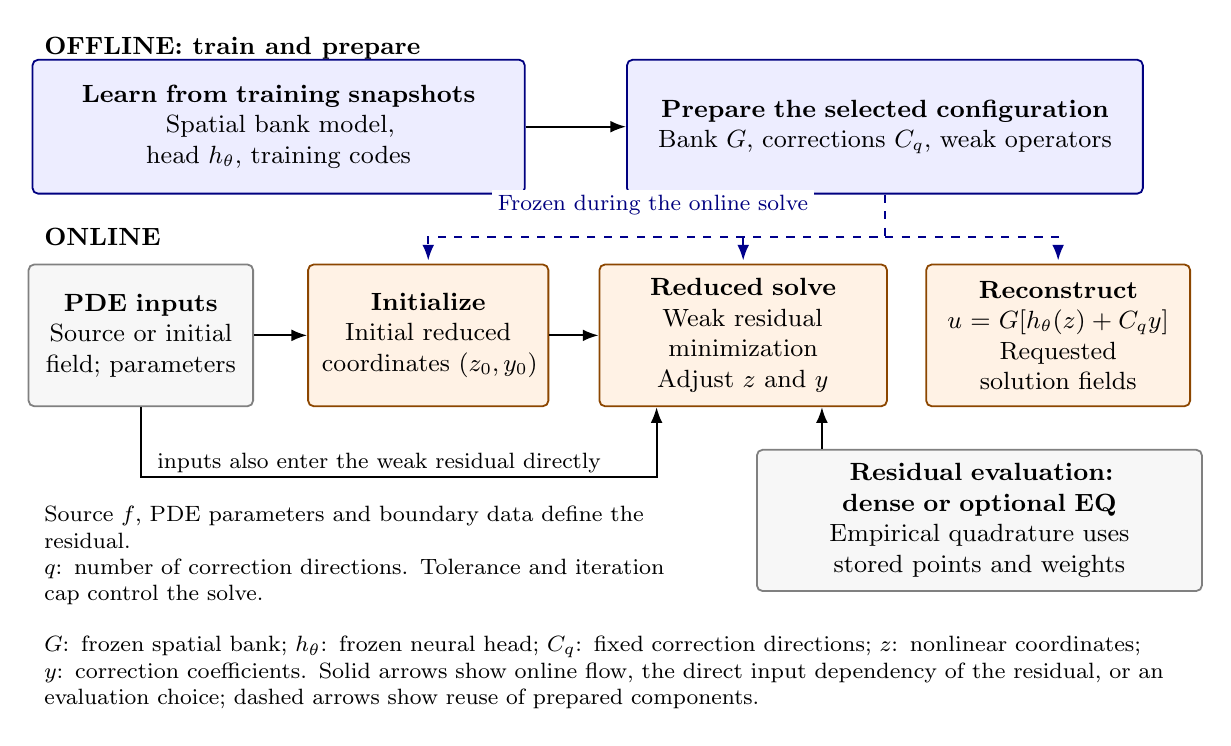
\begin{tikzpicture}[
  font=\small,
  box/.style={draw=black!50,rounded corners=2pt,align=center,inner sep=5pt,line width=.65pt},
  frozen/.style={box,fill=blue!7,draw=blue!50!black},
  online/.style={box,fill=orange!10,draw=orange!55!black,minimum height=18mm},
  input/.style={box,fill=black!3,minimum height=18mm},
  arr/.style={-{Latex[length=2mm]},line width=.7pt},
  reuse/.style={arr,dashed,draw=blue!55!black}
]
\node[anchor=west,font=\small\bfseries] at (0,3.65) {OFFLINE: train and prepare};
\node[frozen,text width=5.9cm,minimum height=17mm] (train) at (3.1,2.65)
 {\textbf{Learn from training snapshots}\\Spatial bank model, head $\head$, training codes};
\node[frozen,text width=6.2cm,minimum height=17mm] (prepare) at (10.8,2.65)
 {\textbf{Prepare the selected configuration}\\Bank $\bank$, corrections $\corr$, weak operators};
\draw[arr] (train) -- (prepare);
\node[font=\footnotesize,anchor=east,text=blue!50!black,fill=white,inner sep=2pt] at (9.9,1.65)
 {Frozen during the online solve};
\draw[reuse] (prepare.south) -- (10.8,1.25) -- (5,1.25) -- (5,.95);
\draw[reuse] (9,1.25) -- (9,.95);
\draw[reuse] (10.8,1.25) -- (13,1.25) -- (13,.95);
\node[anchor=west,font=\small\bfseries] at (0,.65+0.6) {ONLINE};
\node[input,text width=2.5cm] (in) at (1.35,0)
 {\textbf{PDE inputs}\\Source or initial field; parameters};
\node[online,text width=2.7cm] (init) at (5,0)
 {\textbf{Initialize}\\Initial reduced\\coordinates $(z_0,y_0)$};
\node[online,text width=3.3cm] (solve) at (9,0)
 {\textbf{Reduced solve}\\Weak residual minimization\\Adjust $z$ and $y$};
\node[online,text width=3.0cm] (out) at (13,0)
 {\textbf{Reconstruct}\\$u=\bank[\head(z)+\corr y]$\\Requested\\solution fields};
\draw[arr] (in) -- (init);
\draw[arr] (init) -- (solve);
\draw[arr] (in.south) -- (1.35,-1.8) -- (7.9,-1.8) -- (solve.south -| 7.9,0);
\node[font=\footnotesize,anchor=south west,inner sep=1.5pt] at (1.5,-1.8)
 {inputs also enter the weak residual directly};
\node[box,fill=black!3,text width=5.3cm] (eq) at (12.0,-2.35)
 {\textbf{Residual evaluation: dense or optional EQ}\\Empirical quadrature uses stored points and weights};
\draw[arr] (eq.north -| 10,0) -- (solve.south -| 10,0);
\node[align=left,text width=8.2cm,anchor=north west,font=\footnotesize] at (0,-2.05)
 {Source $f$, PDE parameters and boundary data define the residual.\\$q$: number of correction directions. Tolerance and iteration cap control the solve.};
\node[align=left,text width=14.4cm,anchor=north west,font=\footnotesize] at (0,-3.7)
 {$\bank$: frozen spatial bank; $\head$: frozen neural head;
 $\corr$: fixed correction directions; $z$: nonlinear coordinates;
 $y$: correction coefficients. Solid arrows show online flow, the direct input dependency of the residual, or an evaluation choice;
 dashed arrows show reuse of prepared components.};
\end{tikzpicture} {}}
\caption{Offline preparation (blue) and online solution (orange).
The PDE input supplies both initialization and the weak residual.
Linear-PDE corrections are eliminated analytically; time-dependent
problems repeat the reduced step. EQ is used only for 2D Burgers.}
\label{fig:arch}
\end{figure}


\section{Experimental configuration and reproducibility}
\label{app:training-schedule}\label{app:provenance}
Tables~\ref{tab:problems} and \ref{tab:spec} identify the two-dimensional
studies and Table~\ref{tab:config3d} the three-dimensional ones. Within each study,
training precedes evaluation and the selected bank, head and correction
directions remain frozen. Deployment changes reduced coordinates, not
network weights. Recorded training configurations and available offline
costs are retained with the source evidence; unrecorded training costs
are not inferred.
%
% GENERATED by paper/gen_headline.py from the wide bank training record -- do not edit.
The wide heat bank of Table~\ref{tab:headline} is a random-Fourier-feature coordinate network (32 features, scale 1.5, width 256, $R=128$) trained for 80000 steps (learning rate 0.001, 64 states $\times$ 2048 points per batch, gradient clip 1, exact coefficient refit every 10000 steps), then a head of width 256 with $k=8$ for 80000 steps (learning rate 0.0005, 128 states per batch), on 512 training draws at $64^2$ with 16 validation draws; its validation projection floor is 0.11\,\%. {}

\begin{table}[htbp]
\centering
\caption{Training configurations of the frozen checkpoints, transcribed from
the committed configuration and code files of each study (paths and
SHA256 in \texttt{evidence/training-configs-2026-09-21}).}
\label{tab:training-all}
\resizebox{\linewidth}{!}{%
% GENERATED by paper/gen_training_appendix.py from evidence/training-configs-2026-09-21 -- do not edit.
\scriptsize
\begin{tabular}{@{}llp{3.2cm}p{3.4cm}p{2.2cm}p{2.0cm}p{2.4cm}@{}}
\toprule
Model & Stage & Network & Optimiser, learning rate & Steps & Batch & Training data \\
\midrule
Burgers 2D ($k=16$, $R=512$) & bank & 128 Fourier features (scale 4), width 1024, 2 layers & AdamW, wd $10^{-5}$, warm-up + cosine $10^{-3}\to10^{-5}$ & 300000 & all states $\times$ 4096 points & 16384 states of 576 trajectories \\
 & head & width 512, 2 layers & Adam, warm-up + cosine $10^{-3}\to10^{-5}$ & 200000 & 4096 states & 131072 states of 4608 trajectories \\
Poisson 2D ($k=32$, $R=512$) & bank & 64 Fourier features (scale 4), width $R$, 2 layers & Adam, four phases at $10^{-3}$, $3{\times}10^{-4}$, $3{\times}10^{-4}$, $10^{-4}$ & 100000, 40000, 30000, 30000 & 64 sources $\times$ 4096 points & 2611 fit / 461 validation sources \\
 & head & width 128, 2 layers & Adam, $10^{-3}$ & 150000 (full batch) & all & as bank \\
Poisson 2D ($k=16$, $R=128$) & bank + head & 64 Fourier features, $g$ and $h$ width 128, 2 layers & Adam; staged from an $R=64$ model (bank, head, joint at $3{\times}10^{-4}$, $3{\times}10^{-4}$, $10^{-4}$) & 40000, 30000, 20000 after widening & 64 sources $\times$ 4096 points & 512 training sources \\
L-shape ($k=16$, $R=512$) & bank / head & 64 Fourier features (scale 4), 2 layers; head width 128, 2 layers & as Poisson $k=32$ & 100000, 40000, 30000, 30000; head 150000 & 64 sources $\times$ 4096 points & 2611 fit / 461 validation sources \\
Poisson 3D ($k=16$, $R=128$) & bank / head & 64 Fourier features (scale 1.5), widths 256; head width 256 + skip & Adam, cosine (floor 0.03); $10^{-3}$ bank, $5{\times}10^{-4}$ head & 150000 / 100000 & 64 states $\times$ 2048 points / 128 states & 512 training / 16 validation fields \\
\bottomrule
\end{tabular} {}}
\end{table}

%
% GENERATED by paper/gen_training_appendix.py -- do not edit.
\paragraph{Full-order and solver details.} The Burgers FOM is Newton's method with BiCGStab inner solves (at most 200 iterations, Jacobian--vector products by forward-mode differentiation) preconditioned by the exact inverse of the implicit Helmholtz operator $(I+\Delta t\,\nu\,\lambda)^{-1}$ (advection dropped); Newton stops when the residual norm falls below the nonlinear tolerance times the previous state's norm, or after 20 iterations, and always takes the full step (no line search or damping). Each named setting fixes $\Delta t$, the nonlinear and the linear tolerance. On the L-shape the vanishing factor is $4\min(x,\,y,\,d_{\mathrm{right}},\,d_{\mathrm{top}},\,d_{\mathrm{corner}})$ with the distances to the outer right and top edges and to the re-entrant corner, and the test space is the $M$ lowest eigenvectors of the five-point operator on the masked grid, computed by shift-invert Lanczos and scaled as $\tests=\rowscale^{-1}\Phi\T$ ($M=257$; $M=1024$ for the $q=R$ solve). The quadratic predictor of the $4096^2$ Burgers rows forms the linear extrapolation $2w_n-w_{n-1}$ and, from the third step on, the quadratic one $3w_n-3w_{n-1}+w_{n-2}$, evaluates the residual norm of the current code and both candidates in one batched call and starts the solve from the smallest. {}

\paragraph{Three-dimensional heat, new bank.} The bank of the Heat (new
bank) rows ($R=\nHeatNewR$) was trained with a code-free
variable-projection trainer that eliminates the coefficients exactly;
its projection floor is $\nHeatNewFloor\,\%$. Its arms were fixed by a
rule registered before the sealed cohort was opened.

\begin{table}[htbp]
\centering
\caption{Problem specification. Cohort and reduced sizes are read from the run
configurations where recorded. The Burgers sealed cohort has been opened
and is reported in Table~\ref{tab:sealed}; other rows describe their
recorded development and validation cohorts.}
\label{tab:problems}
\resizebox{\linewidth}{!}{%
% GENERATED by paper/gen_tables.py -- do not edit.
% problem specification; numeric fields read from tuning02 config where recorded
\tiny
\begin{tabular}{p{1.5cm}p{3.0cm}p{1.4cm}p{2.0cm}p{1.9cm}p{1.9cm}p{2.3cm}}
\toprule
PDE & equation, domain, boundary & meshes & time stepping & reduced sizes & reference & cohorts \\
\midrule
Burgers 2D & $u_t+u(u_x+u_y)=\nu\Delta u$, $(0,1)^2$, $u|_{\partial\Omega}=0$ & $256^2$--$4096^2$ & $\Delta t=0.005$, backward Euler, sign-upwind & $k=16$, $R=512$ & refined $ 4096^2$, $\Delta t=0.00015625$ & 6 development cases; 32 validation; 64 held-out at $2048^2$, $4096^2$; sealed cohort opened once \\
Poisson 2D & $-\Delta u=f$, $(0,1)^2$, $u|_{\partial\Omega}=0$ & $256^2$--$4096^2$ & none (elliptic) & $k=16$, $R=128$ (original); $k=32$, $R=512$ & exact discrete solution; 2048$^2$ refinement & 12 development sources \\
Heat 2D & $u_t=\kappa\Delta u$, $(0,1)^2$ & $64^2$--$1024^2$ & Crank--Nicolson & $k=8$, $R=32$ & refined-grid reference ($1024^2$/$2048^2$ pair); error includes discretisation & 12 development cases, 3 repetitions; measured in job 3529772; checkpoint lineage: earlier cell, job 3511417 \\
Heat 2D, wide bank & $u_t=\kappa\Delta u$, $(0,1)^2$ & $1024^2$--$4096^2$ & Crank--Nicolson; batched exact-propagator fit & $k=8$, $R=128$ & exact same-grid propagation & 12 development cases; 16 sealed held-out cases, opened once \\
Wave 2D (reflective) & $u_{tt}=c^2\Delta u$, $(0,1)^2$, $u|_{\partial\Omega}=0$ & $64^2$, $256^2$, $1024^2$ & RK4 on the manifold; exact modal propagation for the bank & $k=32$, $R=64$ & exact modal solution & 8 development cases \\
Poisson, L-shape & $-\Delta u=f$, $(0,1)^2\setminus[\tfrac12,1)^2$ & $256^2$--$2048^2$ & none & $k\in\{16,32\}$, $R\in\{256,512,514\}$ & converged discrete solution & 3072 / 256 / 32 sources (train / selection / development) \\
\bottomrule
\end{tabular} {}}
\end{table}

\begin{table}[htbp]
\centering
\caption{Sampled problem families, transcribed from the generator sources named
in the last column (code constants, not run outputs).}
\label{tab:spec}
\resizebox{\linewidth}{!}{%
% GENERATED by paper/gen_tables.py -- do not edit.
% sampling families transcribed from the generator sources named in the last column
\scriptsize\def\UrlBreaks{\do\/\do\-\do\_\do\.\do\:}
\begin{tabular}{@{}p{1.4cm}p{2.7cm}p{6.0cm}p{2.55cm}@{}}
\toprule
PDE & equation and boundary & sampled family (transcribed from the generator source) & source \\
\midrule
Burgers 2D & $u_t+u(u_x+u_y)=\nu\Delta u$ on $(0,1)^2$, $u=0$ on $\partial\Omega$ & $u_0=a\exp(-\lvert x-c\rvert^2/2w^2)$, $c_i\sim U(0.15,0.85)$, $w\sim U(0.05,0.20)$, $a\sim U(0.5,2)$; $\nu\sim\log U(0.01,0.1)$; outputs $t\in\{0.05,\dots,0.25\}$ & \path{experiments/mr-burgers2d/engines.py:params_draw} \\
Poisson 2D & $-\Delta u=f$ on $(0,1)^2$, $u=0$ on $\partial\Omega$ & $f=a\exp(-\lvert x-c\rvert^2/2w^2)$, $c_i\sim U(0.15,0.85)$, $w\sim\log U(0.02,0.1)$, $a\sim U(0.5,2)$ & \path{multistage-precision/ms_parametric.py:sample_params} \\
Poisson, L-shape & same source family on $(0,1)^2\setminus[\tfrac12,1)^2$ & as above; sources centred in the removed quadrant rejected & \path{experiments/lshape} \\
Heat 2D & $u_t=\kappa\Delta u$ on $(0,1)^2$, $\kappa=0.02$ fixed & polynomial-boundary Gaussian family (single\_bc\_poly\_gaussian\_v1); Crank--Nicolson $\Delta t=0.025$ & checkpoint \path{expanded_seed790715} (lineage: linear-bank cell, job 3511417); printed CG measurements: job 3529772 \\
Wave 2D (reflective) & $u_{tt}=c^2\Delta u$ on $(0,1)^2$, $u=0$ on $\partial\Omega$ & compact bump $\times$ Gaussian: half-widths $s_i\sim U(0.36,0.42)$, centre $c_i\sim U(s_i{+}0.025,\,1{-}s_i{-}0.025)$, amplitude $\sim U(0.7,1.3)$, $\sigma_i\sim U(0.12,0.16)$, advective velocity $v_i\sim U(-0.5,0.5)$ (zero every fourth case); speed $c\sim U(0.85,1.15)$ & \path{experiments/multiresolution-wave/audit_dynamics.py:parameter_rows} \\
\bottomrule
\end{tabular} {}}
\end{table}


\subsection{Headline settings, times and timing protocol}
\label{app:cg-current}\label{app:main-experiment-details}
Table~\ref{tab:headline-times} gives the settings and measured times
behind every row of Table~\ref{tab:headline}. Every cost and error come
from the same invocation. Timings use GPU warm-up and synchronisation,
double precision and the highest matrix-multiplication precision; all
repetitions, including outliers, enter the median, and no time is
borrowed from another allocation. Requested full fields and
initialisation are charged; host transfer is included only where the
table says complete query. For the held-out Burgers rows, an independent
restricted-grid recomputation of the errors disagreed with the full-grid
value by more than 5\,\% on $\nBurgGateBadTwentyFortyEight/\nBurgGateRowsTwentyFortyEight$
($2048^2$) and $\nBurgGateBadFortyNinetySix/\nBurgGateRowsFortyNinetySix$
($4096^2$) case--arm rows; per-arm cohort worsts agree within
$\nBurgGateWorstPct\,\%$ and the full-grid recomputation is exact. For Burgers at $256^2$ no quadrature rule passed the pre-registered
re-draw procedure (its pick failed the confirmation draw), so
Table~\ref{tab:headline} has no confirmed-rule row there; a post-hoc
follow-up rule with an exact first time step passes all
\nEqcFollowDraws{} draws of two jobs and gives $\nEqcFollowErr\,\%$ at
$\nEqcFollowS\times$ against the same Newton--BiCGStab rule. For Burgers at $4096^2$, copying the six
double-precision output fields to the host adds about
$\nBurgHostGapMs$\,ms to every arm. The Poisson and three-dimensional heat CG comparators are
unpreconditioned; heat CG is warm-started from the previous time level. The Heat2D rows use checkpoint
\texttt{expanded\_seed790715}; Table~\ref{tab:problems} separates that
checkpoint's lineage from the job that produced the printed
measurements.

\paragraph{Model and table annotations.}
Heat (wide bank) is a separately trained frozen model with a
128-function bank ($q=32$ accurate); over evolved times its accurate
error is $\nHeatWideAccEvolved\,\%$ ($\nHeatWideBatchedAccEvolved\,\%$
batched; the batched fit: Table~\ref{tab:headline-times}); Heat (new
bank) ($q=\nHeatNewQ$ accurate; Table~\ref{tab:config3d}): at most $\nHeatNewAccEvolved\,\%$
($\nHeatNewBatchedAccEvolved\,\%$ batched) over evolved times;
$^{n}$\,\nHeatNewNonstat{} solve (one step of one case) missed its
stationarity rule, so no speedup is given.

\paragraph{Burgers rule identities.} Burgers accurate
quadrature: $^{s}$\,stored rule of job \provEqtopLadderJob{}
($m=\nEqcLaneRuleM$; not the $q=256$ rule of Table~\ref{tab:eqladder}),
not confirmed on re-draws: it fails the confirmation draw at $256^2$;
$^{x}$\,its nodes with weights refit at $512^2$
($m=\nEqcRowRuleMFiveTwelve$), one held-out draw, not re-drawn (with
unrefit weights they pass \nEqcScaledPassFiveTwelve{} of
\nEqcScaledDrawsFiveTwelve{} re-draws); $^{\ell}$\,$63{\times}63$
lattice rule: at $2048^2$ it clears the re-draw bar by only
$\nEqcLatMargin$ ($\rho_{\max}=\nEqcLatConfRho$ vs.\ $\nEqcBar$).
At $4096^2$, a later confirmation draw fails the bar. A variant with
an exact first step passes the check but loses the speed advantage;
$^{v}$\,confirmed by the pre-registered re-draw procedure ($1024^2$: thin
margin, $\rho_{\max}=\nEqcConfRhoTenTwentyFour$; none passes at $256^2$,
Appendix~\ref{app:cg-current}); $^{d}$\,dense residual. The earlier Burgers model has one setting and
may exit on a stall; its rule-selected FOM is the relaxed Newton setting
($10^{-2}/0.5$), the FOM setting can differ between meshes of a series. $^{h}$\,64 held-out cases never used for
selection (not the sealed final cohort); at $2048^2$ the development-chosen
$M=544$ setting was not run on them, so the $M=1088$ setting is shown.

The separate bank follow-up also missed its combined held-out accuracy
and speed target. The committed follow-up handoff is retained with its
source hash in \texttt{evidence/readability-2026-09-22}.

\begin{table}[htbp]
\centering
\caption{Settings and median times for exactly the rows of
Table~\ref{tab:headline}, using the same FOM setting and allocation.
Settings give $q$, or $q/M/m$ where recorded; D means dense and
$^{*}$ an exact first step. Times include initialization, solution and
requested device fields;
$^{c}$ includes host transfers as well. The last column gives
complete-query speedups (accurate / fast) where separately measured.
$^{n}$ marks a nonstationary solve whose speedup is omitted from
Table~\ref{tab:headline}. The batched heat fit treats output times
independently using exact weak-moment propagation.}
\label{tab:headline-times}
\resizebox{\linewidth}{!}{%
% GENERATED by paper/gen_headline.py -- do not edit.
\small
\begin{tabular}{@{}llrrrrrl@{}}
\toprule
Problem & Mesh & Acc.\ setting & Fast setting & Acc.\ ms & Fast ms & FOM ms & Complete-query $S$ \\
\midrule
Poisson 2D & $256^2$ & $256$ & $0$ & 7.12 & 6.70 & 22.29 & --- \\
Poisson 2D & $1024^2$ & $256$ & $0$ & 4.32 & 3.94 & 60.02 & --- \\
Poisson 2D & $2048^2$ & $256$ & $0$ & 5.47 & 5.35 & 397.80 & 28.7 / 28.8 \\
Poisson 2D & $4096^2$ & $256$ & $0$ & 16.92 & 16.74 & 1954.80 & 32.7 / 33.2 \\
Poisson, L-shape 2D$^{c}$ & $256^2$ & $64$ & $0$ & 3.03 & 2.88 & 11.64 & --- \\
Poisson, L-shape 2D$^{c}$ & $512^2$ & $64$ & $0$ & 4.80 & 4.72 & 29.13 & --- \\
Poisson, L-shape 2D$^{c}$ & $1024^2$ & $128$ & $0$ & 5.81 & 5.67 & 48.70 & --- \\
Poisson, L-shape 2D$^{c}$ & $2048^2$ & $128$ & $0$ & 18.75 & 18.66 & 318.22 & --- \\
Heat 2D & $64^2$ & --- & single & --- & 11.23 & 2.50 & --- \\
Heat 2D & $256^2$ & --- & single & --- & 11.34 & 6.94 & --- \\
Heat 2D & $1024^2$ & --- & single & --- & 12.21 & 59.18 & --- \\
Heat (wide bank) 2D & $1024^2$ & $32$ & $0$ & 27.33 & 27.77 & 43.51 & --- \\
Heat (wide bank) 2D & $2048^2$ & $32$ & $0$ & 27.97 & 28.42 & 272.55 & --- \\
Heat (wide bank) 2D & $4096^2$ & $32$ & $0$ & 31.68 & 32.19 & 1139.83 & --- \\
Heat (wide bank, batched fit) 2D & $1024^2$ & $32$ & $0$ & 3.13 & 3.36 & 43.51 & --- \\
Heat (wide bank, batched fit) 2D & $2048^2$ & $32$ & $0$ & 4.54 & 4.78 & 272.55 & --- \\
Heat (wide bank, batched fit) 2D & $4096^2$ & $32$ & $0$ & 11.03 & 11.33 & 1139.83 & --- \\
Burgers 2D & $256^2$ & $256/1088/2560$ & $0/64/1024$ & 746.02 & 40.36 & 31.79 & --- \\
Burgers 2D & $512^2$ & $256/1088/2438$ & $0/64/922$ & 783.33 & 40.49 & 52.92 & --- \\
Burgers 2D & $1024^2$ & $256/1088/\mathrm{D}$ & $0/64/934$ & 22053.85 & 40.27 & 81.31 & --- \\
Burgers 2D & $2048^2$ & $256/544/3969$ & $0/64/1024$ & 124.15 & 29.48 & 122.76 & 0.99 / 2.01 \\
Burgers 2D & $4096^2$ & $256/1088/3969$ & $0/64/1024$ & 107.51 & 40.73 & 523.85 & 2.18 / 2.68 \\
Burgers (held-out cases) 2D & $2048^2$ & $256/1088/3969$ & $0/64/1024$ & 114.91 & 29.19 & 164.43 & 1.28 / 2.49 \\
Burgers (held-out cases) 2D & $4096^2$ & $256/1088/3969$ & $0/64/1024$ & 99.96 & 40.60 & 537.39 & 2.28 / 2.74 \\
Burgers, confirmed rule 2D & $512^2$ & $256/1088/3969^{*}$ & $0/64/1024$ & 194.97 & 23.62 & 17.74 & --- \\
Burgers, confirmed rule 2D & $1024^2$ & $256/1088/3969$ & $0/64/1024$ & 108.58 & 25.00 & 34.69 & --- \\
Burgers (earlier model) 2D & $1024^2$ & --- & single & --- & 41.68 & 68.04 & --- \\
Poisson 3D & $32^3$ & $96$ & $0$ & 2.63 & 2.49 & 2.47 & --- \\
Poisson 3D & $64^3$ & $96$ & $0$ & 3.36 & 3.22 & 4.46 & --- \\
Poisson (dev. sources) 3D & $128^3$ & $96$ & $0$ & 1.86 & 1.80 & 12.55 & 2.70 / 2.66 \\
Poisson (dev. sources) 3D & $256^3$ & $96$ & $0$ & 6.08 & 5.95 & 140.87 & 4.18 / 4.21 \\
Heat (new bank) 3D & $32^3$ & $288$ & $0$ & 58.16 & 25.41 & 3.33 & --- \\
Heat (new bank) 3D & $64^3$ & $288$ & $0$ & 58.69$^{n}$ & 25.45 & 5.23 & --- \\
Heat (new bank) 3D & $128^3$ & $288$ & $0$ & 62.03 & 28.25 & 17.44 & --- \\
Heat (new bank, batched fit) 3D & $32^3$ & $288$ & $0$ & 5.36 & 5.88 & 3.33 & --- \\
Heat (new bank, batched fit) 3D & $64^3$ & $288$ & $0$ & 5.54 & 6.14 & 5.23 & --- \\
Heat (new bank, batched fit) 3D & $128^3$ & $288$ & $0$ & 7.84 & 8.30 & 17.44 & --- \\
\bottomrule
\end{tabular} {}}
\end{table}

\begin{table}[htbp]
\centering
\caption{Burgers 2D correction settings from one frozen model at $256^2$,
test count fixed at $M=\nQxmFixedM$, dense residual, one allocation. Errors are worst
evolved same-grid percentages on development cases; times are paired
median GPU query times. All rows meet the stopping rule.}
\label{tab:ladder-main}
%
% GENERATED by paper/gen_tables.py -- do not edit.
% fixed test space; same checkpoint and job 3780177
\small
\begin{tabular}{rrr}
\toprule
Correction rank $q$ & Relative $L^2$ error (\%) & GPU query time (ms) \\
\midrule
0 & 1.2657 & 848.0 \\
64 & 1.0593 & 1359.4 \\
128 & 0.8711 & 1886.5 \\
256 & 0.5194 & 4377.9 \\
\bottomrule
\end{tabular} {}
\end{table}

\begin{table}[htbp]
\centering
\caption{Three-dimensional configurations, read from the run records.
Domains are the unit cube with homogeneous Dirichlet data, except
Navier--Stokes, which is periodic. Burgers and Navier--Stokes appear in
Table~\ref{tab:failures}.}
\label{tab:config3d}
\resizebox{\linewidth}{!}{%
% GENERATED by paper/gen_headline.py -- do not edit.
\scriptsize
\begin{tabular}{@{}lllp{3.3cm}p{3.6cm}l@{}}
\toprule
Problem & Mesh & Cases & Correction ranks & Named FOM & Residual \\
\midrule
Burgers 3D & $32^3$ & 32 final & 0, 192 & Newton--BiCGStab, $\Delta t=0.01$ & dense \\
Poisson 3D & $32^3$, $64^3$ & 64 final & 0, 32, 96 ($k=16$) & CG, rtol $10^{-2}$, no preconditioner & dense \\
Heat 3D (new bank) & $32^3$, $64^3$, $128^3$ & 64 sealed final (all times) & 0, 288 ($k=32$, $R=320$) & CN--CG, setting per row by the rule; named $\Delta t=0.025$, rtol $10^{-6}$ & exact (linear) \\
Navier--Stokes 3D & $32^3$ periodic & 32 final & 0, 32, 64, 128, 256 ($k=64$, $R=1536$, $M=2048$) & CNAB2, $\Delta t=0.01$ & dense \\
\bottomrule
\end{tabular} {}}
\end{table}

Three-dimensional Poisson ($-\Delta u=f$, Gaussian sources), heat
($u_t=\kappa\Delta u$, Gaussian initial fields) and scalar Burgers
($u_t+u(u_x+u_y+u_z)=\nu\Delta u$, backward Euler, sign-upwind) are posed
on the unit cube with zero Dirichlet walls and extend the operators of
Appendix~\ref{app:method} across three axes. Navier--Stokes uses
periodic vector fields, an incompressibility projection and the CNAB2
integrator; its FOM is not a CG solve. All four three-dimensional problems are evaluated on held-out final
cohorts whose settings were frozen beforehand.

\paragraph{Source records.}
The repository retains configurations, checkpoints, case-level outputs,
timing repetitions and audits. The manifests in \texttt{tables/}
identify the source commits and hashes for each generated value;
\texttt{headline-provenance.json} covers the main comparison tables.
The Burgers training and evaluation parameters were regenerated and
checked for overlap: none was found. The check and its output are in
\texttt{evidence/burgers-train-eval-overlap-2026-09-21}.

\subsection{Reproduced NM-ROM baseline}
\label{app:nmrom-baselines}
The shallow masked-autoencoder NM-LSPG of \citet{KimChoi2022NMROM}
passed its reproduction gate on the third registered attempt on the
published Burgers benchmark: median $\nBaseGateMedian\,\%$ against a
$\nBaseGateBar\,\%$ gate (\nBaseGateAct{} activation). Its
hyper-reduction did not pass the reproduction gate. Table~\ref{tab:nmrom-baselines}
therefore uses dense residuals for every method. Our reference path
uses tolerance $10^{-6}$ and $M=4(k+q)$.
The published encoder width, $2n$, exceeds device memory. At $512^2$,
the width-capped encoder ($\nBaseKimWidth$) trained for only
\nBaseKimEpochs{} epochs within $\nBaseKimWall$\,s. Its error thus
reflects a training constraint as well as the representation and solve.
Exploratory timings and failed hyper-reduction runs remain in the
repository evidence.

\section{Validation of the correction and quadrature studies}


\begin{table}[htbp]
\centering
\caption{The sealed cohort (job \nSealedJob, \provSealedGpu),
opened once after every choice was frozen. Top: per rung of the dense
$M=4(k+q)$ ladder, the original model's sealed worst evolved error and device
time, the seed mean $\pm$ sample standard deviation on the sealed and the
development cohort, the pre-registered sealed-over-development ratio of seed means
(raw and difficulty-normalised) and the converged count over the
\nSealedCheckpoints{} checkpoints. Bottom: per-checkpoint verdicts. The
original model's $q=0$ rung is a single sealed case converged to a wrong branch
(gradient exit, zero budget exits); the pre-registered ratio criterion fails
at $q=0$ for the original model alone (\nSealedCtwoIncQzeroRatio) and the
convergence criterion fails on \nSealedUnconvergedPlain. Top-rank sealed errors per checkpoint: \nSealedTopPerCheckpoint.}
\label{tab:sealed}
\resizebox{\linewidth}{!}{%
% GENERATED by paper/gen_tables.py -- do not edit.
% sealed cohort, job 3804465 (A100-40GB), dense M = 4(k+q); sealed worst evolved error per rung for the original model and the seed mean +- sample std beside the development seed mean; C2 ratios from the lane; unconverged rungs marked
\scriptsize
\begin{tabular}{rrrrllrrl}
\toprule
$q$ & $M$ & original model sealed \% & ms & seeds sealed \% & seeds development \% & sealed / dev & normalised & converged \\
\midrule
0 & 64 & 10.1120 & 375.1 & 2.8023 $\pm$ 0.6357 & 2.0002 $\pm$ 0.4986 & 1.40 & 1.41 & 4 of 4 \\
16 & 128 & 1.4617 & 480.8 & 1.7305 $\pm$ 0.1297 & 1.5988 $\pm$ 0.0995 & 1.08 & 1.09 & 4 of 4 \\
32 & 192 & 1.4458 & 540.5 & 1.5044 $\pm$ 0.1422 & 1.3727 $\pm$ 0.1314 & 1.10 & 1.14 & 4 of 4 \\
64 & 320 & 1.3252 & 754.5 & 1.3528 $\pm$ 0.1099 & 1.2130 $\pm$ 0.0580 & 1.12 & 1.13 & 3 of 4 \\
128 & 576 & 1.0964 & 1460.4 & 1.0461 $\pm$ 0.0619 & 0.9562 $\pm$ 0.0264 & 1.09 & 1.17 & 4 of 4 \\
256 & 1088 & 0.6789 & 6725.5 & 0.6188 $\pm$ 0.0345 & 0.4987 $\pm$ 0.1164 & 1.24 & 1.20 & 4 of 4 \\
\bottomrule
\end{tabular} {}}\\[4pt]
\resizebox{\linewidth}{!}{%
% GENERATED by paper/gen_tables.py -- do not edit.
% sealed cohort, per-checkpoint ladder verdicts, job 3804465
\scriptsize
\begin{tabular}{llllllll}
\toprule
checkpoint & job & monotone (evolved) & monotone (all-times) & every setting converged & error span & cost span & secondary criterion \\
\midrule
original & \texttt{3804465} & yes & yes & yes & 14.89$\times$ & 17.93$\times$ & yes \\
first seed & \texttt{3804465} & yes & yes & yes & 3.52$\times$ & 13.25$\times$ & yes \\
second seed & \texttt{3804465} & yes & yes & no & 4.81$\times$ & 13.17$\times$ & no \\
third seed & \texttt{3804465} & yes & yes & yes & 5.22$\times$ & 14.62$\times$ & yes \\
\bottomrule
\end{tabular} {}}
\end{table}

\begin{table}[htbp]
\centering
\caption{The EQ ladder with the cheapest rule passing the primary bar in its
draw per rung, timed in one allocation (job \provEqtopLadderJob, A100 80\,GB),
with its same-job dense twins, and the construction status from the four-draw
replication (job \provEqtopRepJob): confirmed = every re-draw passes, marginal
= only the listed fraction does. Errors are as measured with these rules
(SHA256-identified); they are not properties of the construction above
$q=32$. Ladder rows are read from the study's final summary record.}
\label{tab:eqladder}
\resizebox{\linewidth}{!}{%
% GENERATED by paper/gen_tables.py -- do not edit.
% EQ-ladder job 3780164; construction status from the draw replication (job 3783811)
\scriptsize
\begin{tabular}{rrrrlrrrrrr}
\toprule
$q$ & $m$ & fit states & $\rho_{\max}$ (this draw) & construction status & EQ evolved \% & EQ all \% & EQ ms & dense evolved \% & dense ms & EQ/dense cost \\
\midrule
0 & 1024 & 64 & 0.0153 & confirmed (3 of 3 re-draws) & 1.8891 & 2.5629 & 59.1 & 1.8890 & 292.9 & 0.202 \\
16 & 1024 & 64 & 0.0935 & confirmed (3 of 3 re-draws) & 1.4270 & 2.4806 & 80.6 & --- & --- & --- \\
32 & 1024 & 42 & 0.0533 & confirmed (2 of 2 re-draws) & 1.2493 & 2.3534 & 97.7 & --- & --- & --- \\
64 & 1024 & 25 & 0.0531 & marginal (2 of 6 draws pass) & 1.2275 & 2.1489 & 120.6 & 1.0843 & 624.9 & 0.193 \\
128 & 2048 & 64 & 0.0669 & marginal (4 of 5 draws pass) & 0.8936 & 1.8116 & 246.9 & 0.8930 & 1190.5 & 0.207 \\
256 & 2048 & 64 & 0.1074 & marginal (1 of 5 draws pass) & 0.5389 & 0.9053 & 722.2 & 0.5194 & 3915.1 & 0.184 \\
\bottomrule
\end{tabular} {}}
\end{table}

\begin{table}[htbp]
\centering
\caption{Solver-side controls on Burgers 2D, 32 validation cases,
one allocation: stopping tolerance, EQ node count $m$ and iteration cap,
with full-order settings for scale. Error: worst over
cases and output times of the $L^2$ error against the refined reference,
relative to the initial-field norm, so the full-order rows show their
discretisation error.}
\label{tab:knobs}
%
% GENERATED by paper/gen_tables.py -- do not edit.
% fixed-checkpoint tuning, validation pass, job 3712269
\scriptsize
\begin{tabular}{lrrr}
\toprule
setting & worst \% (32 validation) & device ms & early-stopped \\
\midrule
EQ $m{=}256$, tol $10^{-6}$, cap 180 & 7.245 & 51.0 & 0/96 \\
EQ $m{=}512$, tol $10^{-8}$ & 6.712 & 64.7 & 0/96 \\
EQ $m{=}512$, tol $10^{-3}$ & 6.701 & 41.6 & 0/96 \\
EQ $m{=}512$, cap 2 (early-stopped) & 90.324 & 28.4 & 96/96 \\
FOM Newton $10^{-2}$, $\Delta t{=}0.01$ & 6.807 & 9.9 & 0/96 \\
FOM Newton $10^{-2}$, $\Delta t{=}0.005$ & 35.357 & 17.4 & 0/96 \\
FOM Newton $10^{-4}$, $\Delta t{=}0.005$ & 6.171 & 22.4 & 0/96 \\
FOM Newton $10^{-6}$, $\Delta t{=}0.005$ & 6.172 & 88.3 & 0/96 \\
\bottomrule
\end{tabular} {}
\end{table}

\paragraph{Reading the validation tables.}
Correction rank $q$ is the number of added coefficient directions;
$M$ is the number of weak test modes and $m$ the quadrature node count.
A scheduled ladder changes $M$ with $q$; the main fixed-test-space study
holds $M$ constant. A sealed cohort is opened only after choices are frozen.
Confirmed quadrature passes every independent reconstruction of the rule;
marginal means some reconstructions fail. These statuses concern rule
construction, not just the error of one selected trajectory. Same-grid
error and error against a refined reference measure different quantities. {}

\end{document}
